\documentclass[10pt, xcolor=table]{beamer}
\usepackage{inputenc}
\usepackage{graphicx}
\usepackage {mathtools}
\usetheme{CambridgeUS}
\usecolortheme{dolphin}
\usepackage{booktabs}
\usepackage{lscape}
\usepackage{caption}
\usepackage{tikz}
\usepackage{subcaption}
\usepackage{multicol}
\usepackage{xcolor}
\usepackage{pgfplots}
\usepackage{bm}
\usepackage{xcolor}
\usepackage{multicol}
\usepackage{adjustbox}
\usepackage{ragged2e} % for \justifying command


\setbeamerfont{frametitle}{series=\bfseries}

\newcommand\dc[1]{\textcolor{blue}{#1}}
\setcounter{tocdepth}{3}
\pgfplotsset{compat=1.18}
\usepgfplotslibrary{external} 
\tikzexternalize

\newlength\figureheight
\newlength\figurewidth

\definecolor{myNewColorA}{RGB}{7,47,95}
\definecolor{myNewColorB}{RGB}{210,50,35}
\definecolor{myNewColorC}{RGB}{244,182,0}
\definecolor{myNewColorD}{RGB}{85,168,104}

\setbeamercolor*{palette primary}{bg=myNewColorC}
\setbeamercolor*{palette secondary}{bg=myNewColorB, fg=white}
\setbeamercolor*{palette tertiary}{bg=myNewColorA, fg=white}
\setbeamercolor*{titlelike}{fg=myNewColorA}
\setbeamercolor*{title}{bg=myNewColorA, fg=white}
\setbeamercolor*{item}{fg=myNewColorA}
\setbeamercolor*{caption name}{fg=myNewColorA}

\usefonttheme{professionalfonts}




\usepackage{natbib}
\usepackage{hyperref}
%------------------------------------------------------------
\titlegraphic{
    \begin{figure}
        \centering
        \begin{subfigure}[l]{0.45\textwidth}
            \centering
            
\includegraphics[width=2.5cm,height=1.5cm]{images/Logo_U.T.P.png}
        \end{subfigure}
        \hfill
        \begin{subfigure}[r]{0.45\textwidth}
            \centering
            
\includegraphics[width=3.5cm,height=1cm]{images/logoITISE2023.png}
        \end{subfigure}
    \end{figure}
}

\setbeamerfont{title}{size=\Large\bfseries}
\setbeamerfont{subtitle}{size=\small}
\setbeamerfont{author}{size=\small}
\setbeamerfont{institute}{size=\footnotesize}

\title[Universidad Tecnológica de Pereira]{Multi-Output Variational Gaussian Process for Daily Forecasting of Hydrological Resources}

\author[Julián David Pastrana-Cortés et al.]{%
    \texorpdfstring{
        \begin{tabular}{ccc}
             Julián David Pastrana-Cortés &  David Augusto Cardenas-Peña & \\
             Mauricio Holguín-Londoño &  Germán Castellanos-Dominguez & \\
             \multicolumn{2}{c}{Álvaro Angel Orozco-Gutiérrez} & \\
        \end{tabular}
    }{Julián David Pastrana-Cortés et al.}
}

\institute[ITISE 2023]{9th International conference on Time Series and Forecasting (ITISE 2023)}
\date{July 12th, 2023}

\AtBeginSection[]{
  \begin{frame}
    \vfill
    \centering
    \begin{beamercolorbox}[sep=8pt,center,shadow=true,rounded=true]{title}
      \usebeamerfont{title}\insertsectionhead\par%
    \end{beamercolorbox}
    \vfill
  \end{frame}
}

\justifying
%------------------------------------------------------------

\begin{document}

\frame{\titlepage}

\section*{Motivation}

\begin{frame}{Motivation}

Hydrological forecasting plays a crucial role in planning and operation activities.

\begin{figure}
     \centering
     \begin{subfigure}[b]{0.3\textwidth}
         \centering
         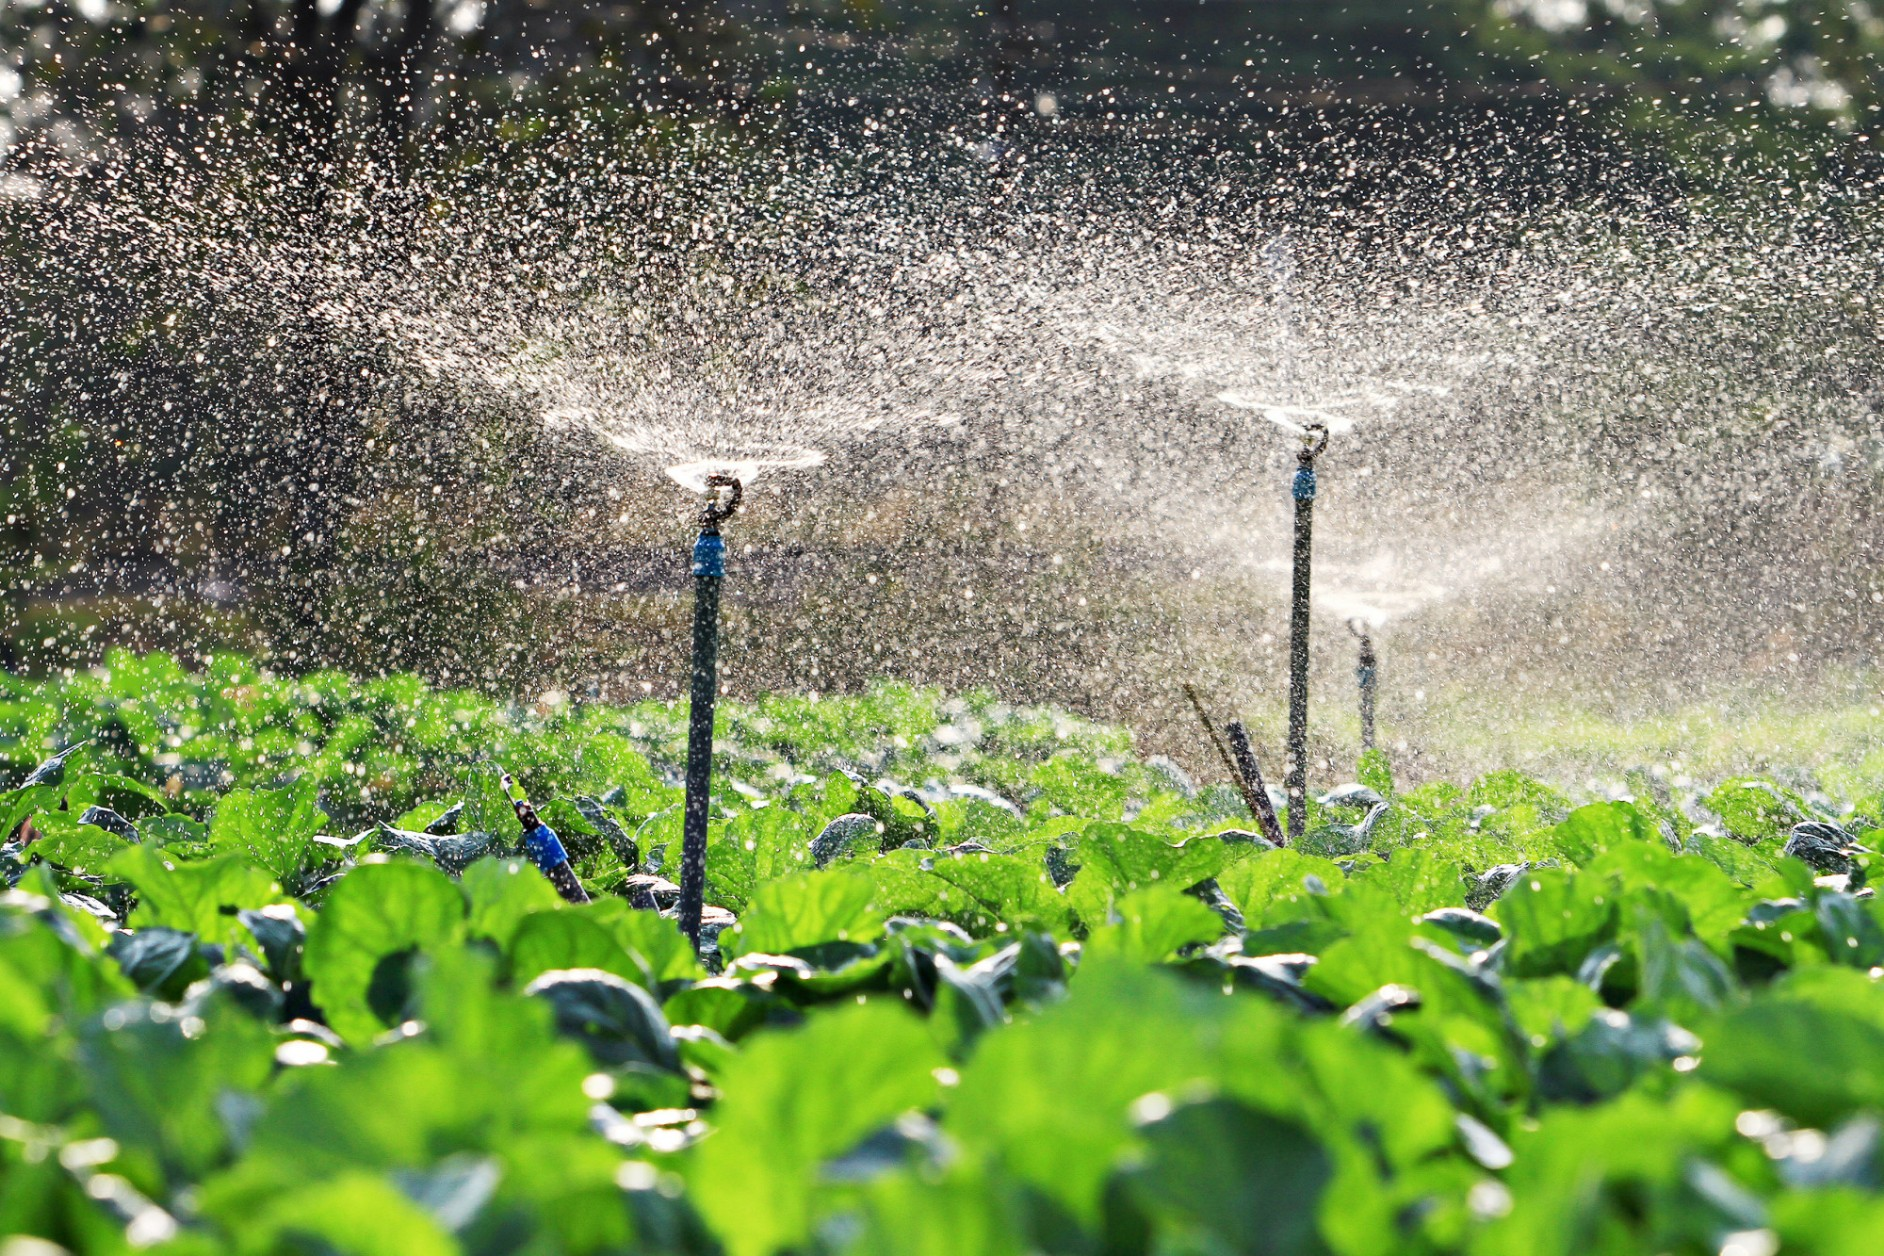
\includegraphics[width=\textwidth, height=4cm]{images/irrigation.jpg}
         \caption{Irrigation}
         \label{fig:y equals x}
     \end{subfigure}
     \hfill
     \begin{subfigure}[b]{0.3\textwidth}
         \centering
         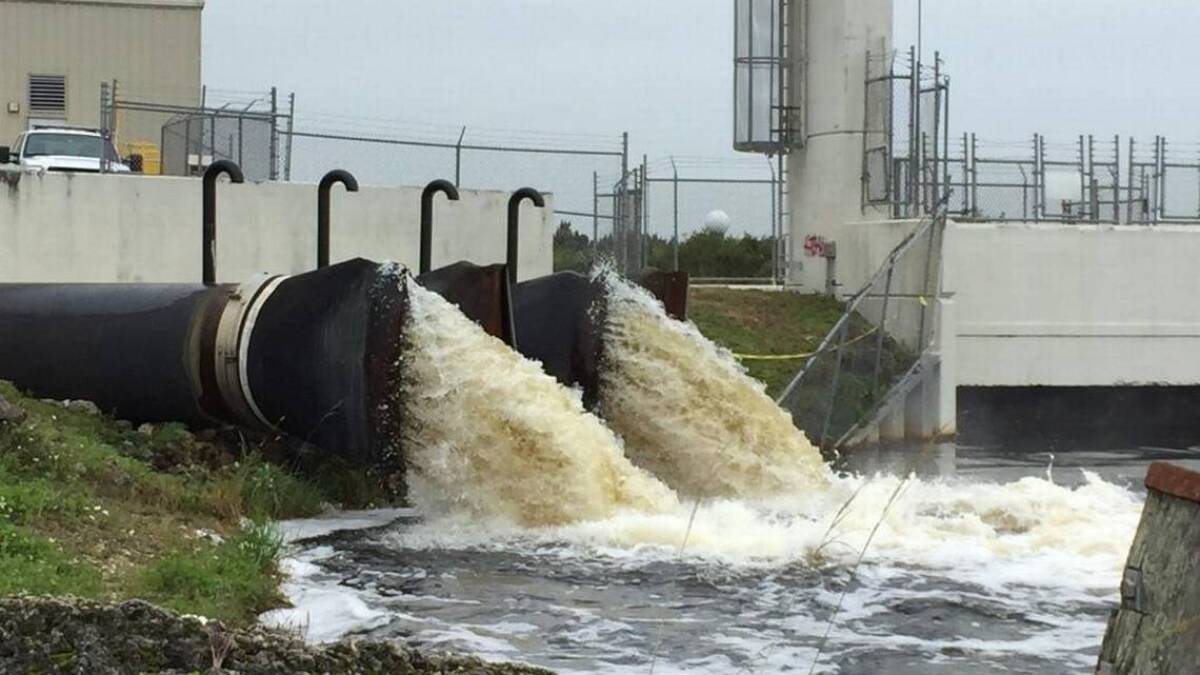
\includegraphics[width=\textwidth, height=4cm]{images/flood_control.jpeg}
         \caption{Flood control}
         \label{fig:three sin x}
     \end{subfigure}
     \hfill
     \begin{subfigure}[b]{0.3\textwidth}
         \centering
         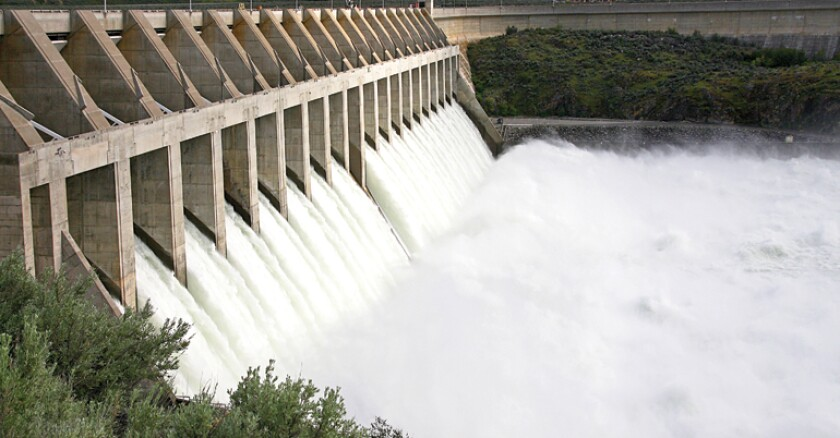
\includegraphics[width=\textwidth, height=4cm]{images/hydro_gen.jpeg}
         \caption{Hydropower generation}
         \label{fig:five over x}
     \end{subfigure}

\end{figure}

\textcolor{myNewColorB}{\textbf{Challenges}}: non-linearities, high stochasticity, and complex water resource patterns.

\end{frame}


\section*{Methods}
\begin{frame}{Gaussian Process Framework}
    A Gaussian Process (GP) is a collection of random variables in which any finite number follows a joint Gaussian distribution. For $D$ tasks, the Multi-Output GP (MOGP) is expressed as follows:

    \begin{equation*}
        \bm{f}(\bm{x}) \sim  \mathcal{GP}(\bm{m}(\bm{x} \mid \bm{\theta}_m),\, \bm{k}(\bm{x}, \bm{x}' \mid \bm{\theta}_k))
    \end{equation*}

    where:
    \begin{itemize}
        \item $\bm{f} : \mathbb{R}^L \rightarrow \mathbb{R}^D$ is the vector-valued function that maps inputs $\bm{x} \in \mathbb{R}^L$
        \item $\bm{m} : \mathbb{R}^L \rightarrow \mathbb{R}^D$ is the mean vector function with parameter vector $\bm{\theta}_m$
        \item $\bm{k}: \mathbb{R}^{L} \times \mathbb{R}^{L} \rightarrow \mathbb{R}^{D \times D}$ is the covariance matrix function with parameter vector $\bm{\theta}_k$
    \end{itemize}
\end{frame}

\begin{frame}{Predictive Distribution}
    Given a training dataset $\mathcal{D} = \{\mathbf{X}, \mathbf{y}\}$ with $\mathbf{X} \in \mathbb{R}^{L \times N}$ and $\mathbf{y} \in \mathbb{R}^{DN}$, and test points $\mathbf{X}_* \in \mathbb{R}^{L \times N_*}$, the predictive distribution is Gaussian with mean vector $\bar{\mathbf{f}}_*$ and covariance matrix $\text{cov}(\mathbf{f}_*)$, where:
    
    \begin{align*}
        \bar{\mathbf{f}}_* &= \mathbf{m}_* + \mathbf{K}_*^{\top} \mathbf{K}_y^{-1} (\mathbf{y} - \mathbf{m}) \\
        \text{cov}(\mathbf{f}_*) &= \mathbf{K}_{**} - \mathbf{K}_*^{\top} \mathbf{K}_y^{-1} \mathbf{K}_*
    \end{align*}
    
    Here:
    \begin{itemize}
        \item $\mathbf{m}_*$ and $\mathbf{m}$ are the mean function evaluations at test and train points, respectively.
        \item $\mathbf{K}$, $\mathbf{K}_{*}$, and $\mathbf{K}_{**}$ are the kernel function evaluations at train-train, train-test, and test-test pairs.
        \item $\mathbf{K}_y = \mathbf{K} + \mathbf{\Sigma}_N \otimes \mathbf{I}_N$, where $\mathbf{\Sigma}_N$ is a diagonal matrix with output noise variances.
        \item $\otimes$ is the Kronecker product between matrices.
    \end{itemize}
\end{frame}


\begin{frame}{Linear Model of Coregionalization}
    The Linear Model of Coregionalization represents each output of a MOGP as a linear combination of $Q$ independent Single Output Gaussian Processes (SOGP):
    
    \begin{equation*}
        \bm{f}(\mathbf{x}) = \sum_{q=1}^Q \mathbf{a}_{q}g_q(\mathbf{x})
    \end{equation*}
    
    The covariance matrix of the MOGP model is given by:
    
    \begin{equation*}\label{eq:MOGP_cov}
        \bm{k}(\mathbf{x}, \mathbf{x}') = \sum_{q=1}^Q \mathbf{B}_q k_q(\mathbf{x}, \mathbf{x}')
    \end{equation*}
    
    Here, $\mathbf{a}_{q} \in \mathbb{R}^D$ is the coefficient vector associated to $q$-th independent SOGP $g_q(\mathbf{x})$, and $\mathbf{B}_q = \mathbf{a}_{q}\mathbf{a}_{q}^\top \in \mathbb{R}^{D \times D}$ is the coregionalization matrix.
\end{frame}

\begin{frame}{Evidence Lower Bound Optimization}

The Variational MOGP (MOVGP) approximates $p(\mathbf{f} \mid \mathbf{X})$, the marginal distribution of output variables $\mathbf{f} = \bm{f}(\mathbf{X}) \in \mathbb{R}^{D N}$, using $M \ll N$ trainable inducing points $\mathbf{Z} \in \mathbb{R}^{L\times M}$ and inducing variables $\mathbf{u} = \bm{f}(\mathbf{Z}) \in \mathbb{R}^{DM}$:

\begin{equation*}\label{prior_aproximation}
    q(\mathbf{f} \mid \mathbf{X}) := \int p(\mathbf{f} \mid \mathbf{X}, \mathbf{u}) q(\mathbf{u}) d\mathbf{u}
\end{equation*}

Assuming a Gaussian distribution $q(\mathbf{u})$, we optimize the parameters $\bm{\theta}_m$, $\bm{\theta}_k$, $\mathbf{\Sigma}_N$, $\mathbf{B}_q$, and $\mathbf{Z}$ using a tractable marginal likelihood bound:

\begin{equation*}\label{marginal_likelihood_bound}
    \log p(\mathbf{y} \mid \mathbf{X}) \geq \sum_{n=1}^N \mathbb{E}_{q(\bm{f}_n \mid \mathbf{x}_n)}[\log p(\bm{y}_n \mid \bm{f}(\mathbf{x}_n))] - \text{KL}[q(\mathbf{u})\parallel p(\mathbf{u})]
\end{equation*}

Here, $\text{KL}[q(\mathbf{u})\parallel p(\mathbf{u})]$ represents the Kullback-Leibler divergence between the distributions $q(\mathbf{u})$ and $p(\mathbf{u})$.
\end{frame}


\section*{Experimental Setup}



\begin{frame}{Dataset}
    The dataset included Useful Volume and Streamflow Contributions from $D = 23$ Colombian reservoirs daily recorded from the last twelve years in kWh. 
    \begin{figure}[htpb]
        \centering 
        \setlength\figurewidth{\columnwidth}
        \setlength\figureheight{0.3\columnwidth}
        % This file was created with tikzplotlib v0.10.1.
\begin{tikzpicture}

\tikzstyle{every node}=[font=\scriptsize]
\definecolor{darkslategray38}{RGB}{38,38,38}
\definecolor{lavender234234242}{RGB}{234,234,242}
% \definecolor{myNewColorC}{RGB}{85,168,104}
% \definecolor{myNewColorA}{RGB}{221,132,82}
% \definecolor{myNewColorA}{RGB}{76,114,176}
\definecolor{lightgray204}{RGB}{204,204,204}

\begin{axis}[
width=\figurewidth,%
height=\figureheight,%
axis background/.style={fill=lavender234234242},
axis line style={white},
legend cell align={left},
legend columns=3, 
legend style={
  fill opacity=0.8,
  draw opacity=1,
  scale=0.01,
  text opacity=1,
  at={(0.03,0.97)},
  anchor=north west,
  legend pos=south west,
  draw=lightgray204,
  fill=lavender234234242
},
log basis y={10},
%tick align=outside,
%unbounded coords=jump,
x grid style={white},
xmajorgrids,
%xmajorticks=false,
xmin=1.8687, xmax=1.9024,
xtick style={color=darkslategray38},
xtick={1.8687,1.8718,1.8748,1.8779,1.8809,1.8840,1.8871,1.8901,1.8932,1.8962,1.8993,1.9024,1.9051},
xticklabels={Mar,Apr,May,Jun,Jul,Aug,Sep,Oct,Nov,Dec,Jan,Feb,},
y grid style={white},
ymajorgrids,
%ymajorticks=false,
ymin=24464.4867138818, ymax=82949446.016724,
ymode=log,
ytick style={color=darkslategray38},
ylabel=kWh,
%ytick={100000,1000000,10000000},
%yticklabels={
%  \(\displaystyle {10^{3}}\),
%  \(\displaystyle {10^{4}}\),
%  \(\displaystyle {10^{5}}\),
%  \(\displaystyle {10^{6}}\),
%  \(\displaystyle {10^{7}}\),
%  \(\displaystyle {10^{8}}\),
%  \(\displaystyle {10^{9}}\)
%}
]
\addplot [semithick, myNewColorA]
table [x expr=\thisrowno{0}/10000, y expr = \thisrowno{1}] {%
18687 7201100
18688 12536000
18689 14551800
18690 3819100
18691 8181500
18692 8693300
18693 8878300
18694 4291500
18695 7283800
18696 13894300
18697 6374300
18698 11799700
18699 17244800
18700 16945600
18701 20335500
18702 35529100
18703 25367200
18704 23256900
18705 24520700
18706 27804300
18707 25012900
18708 14197500
18709 15949500
18710 20473300
18711 14540000
18712 8862600
18713 11913900
18714 10024100
18715 11701300
18716 10484700
18717 7264100
18718 10433500
18719 4393900
18720 8520000
18721 9693300
18722 8008200
18723 3319000
18724 9067300
18725 11091000
18726 13095000
18727 10311500
18728 7661700
18729 10008300
18730 14890400
18731 8433400
18732 8929500
18733 7370400
18734 10079200
18735 8386200
18736 8122400
18737 3602500
18738 6161700
18739 9012200
18740 35400
18741 6138100
18742 7201100
18743 6185300
18744 1917400
18745 5114400
18746 18855100
18747 37092100
18748 29335900
18749 37107900
18750 42572700
18751 51230500
18752 57325300
18753 57222900
18754 50348600
18755 48328800
18756 46167300
18757 47982400
18758 50171400
18759 39635600
18760 30210000
18761 26729500
18762 16524300
18763 20134700
18764 17170000
18765 28717800
18766 24032500
18767 17370800
18768 14815600
18769 14981000
18770 11965100
18771 9362600
18772 16949500
18773 16362900
18774 16280200
18775 18945700
18776 30438300
18777 39848200
18778 39797000
18779 37690600
18780 32918700
18781 27079900
18782 27745300
18783 20311900
18784 14043900
18785 16205400
18786 18981100
18787 26520800
18788 31946200
18789 31540700
18790 36466100
18791 41761600
18792 30973800
18793 42198700
18794 49328900
18795 44887700
18796 32206100
18797 25442000
18798 41667100
18799 56077200
18800 48179200
18801 36387400
18802 30899000
18803 28418500
18804 24386900
18805 17193600
18806 15882600
18807 17335400
18808 14295900
18809 14095100
18810 12606800
18811 13291900
18812 16103000
18813 7543600
18814 9531900
18815 15091200
18816 11114600
18817 17114900
18818 21020600
18819 16788100
18820 10126400
18821 11469000
18822 20622900
18823 22949800
18824 15248700
18825 19351200
18826 16607000
18827 12866700
18828 14303800
18829 17307800
18830 33840000
18831 51541600
18832 36111800
18833 27194100
18834 27414600
18835 29257200
18836 28103600
18837 17130700
18838 17894500
18839 20418200
18840 16859000
18841 15866800
18842 22410400
18843 16697600
18844 16764500
18845 11752500
18846 15374700
18847 13437600
18848 27099600
18849 23914400
18850 29871400
18851 30398900
18852 23623100
18853 24284500
18854 26064100
18855 24961700
18856 39753700
18857 38170900
18858 26339700
18859 38344200
18860 39017400
18861 39017400
18862 39017400
18863 25044400
18864 21520600
18865 19953600
18866 13122600
18867 12347000
18868 23682100
18869 26296400
18870 14788000
18871 12973000
18872 26784600
18873 7929500
18874 9358700
18875 7669600
18876 10417800
18877 13961200
18878 11988700
18879 10929600
18880 8988600
18881 4366300
18882 10874500
18883 15248700
18884 14366800
18885 9094900
18886 8201100
18887 12476900
18888 7252300
18889 6575100
18890 8390100
18891 6791600
18892 10079200
18893 8401900
18894 13784100
18895 15390400
18896 11201300
18897 17059800
18898 9181500
18899 6976700
18900 6913700
18901 11807600
18902 11496600
18903 7012100
18904 5425400
18905 5756200
18906 5516000
18907 9618500
18908 8464900
18909 6543600
18910 6256200
18911 9779900
18912 26859400
18913 29143000
18914 22749000
18915 14925800
18916 18366900
18917 22599400
18918 27698000
18919 23331700
18920 21949800
18921 13878500
18922 17823600
18923 19103200
18924 18878800
18925 26670400
18926 19741000
18927 36792900
18928 31552500
18929 27485400
18930 32249400
18931 45438900
18932 39194600
18933 38993800
18934 35501500
18935 44848400
18936 46970500
18937 54777900
18938 49423400
18939 40198600
18940 28812300
18941 34422700
18942 34434500
18943 32895100
18944 26005000
18945 21611200
18946 20678000
18947 15764500
18948 15110900
18949 13945500
18950 16248700
18951 10724900
18952 13914000
18953 23253000
18954 15953400
18955 25977500
18956 25800300
18957 28501200
18958 22898600
18959 19008700
18960 19768600
18961 16268400
18962 11508400
18963 7622400
18964 11957200
18965 8370400
18966 5323100
18967 6878200
18968 7626300
18969 5559300
18970 8142100
18971 3468700
18972 5913600
18973 5929400
18974 4393900
18975 4512000
18976 5114400
18977 3181200
18978 2842600
18979 4035600
18980 4090700
18981 2767800
18982 nan
18983 7118400
18984 6468800
18985 4897800
18986 4307300
18987 885900
18988 6386100
18989 7295600
18990 7653900
18991 8551500
18992 3826900
18993 6579000
18994 1366200
18995 511800
18996 5712800
18997 1185100
18998 nan
18999 385800
19000 nan
19001 1523700
19002 1956800
19003 nan
19004 3319000
19005 240200
19006 3248200
19007 4968700
19008 nan
19009 3484400
19010 4212800
19011 1779600
19012 nan
19013 196900
19014 196900
19015 3697000
19016 1704800
19017 3917500
19018 2563100
19019 4031700
19020 nan
19021 nan
19022 nan
19023 nan
19024 nan
19025 nan
19026 nan
19027 nan
19028 nan
19029 nan
19030 nan
19031 nan
19032 nan
19033 nan
19034 nan
19035 nan
19036 nan
19037 nan
19038 nan
19039 nan
19040 nan
19041 nan
19042 nan
19043 nan
19044 nan
19045 nan
19046 nan
19047 nan
19048 nan
19049 nan
19050 nan
19051 nan
};
\addplot [semithick, myNewColorB]
table [x expr=\thisrowno{0}/10000, y expr = \thisrowno{1}] {%
18687 4163100
18688 5060100
18689 4124100
18690 3863800
18691 4353600
18692 3016800
18693 2522800
18694 5998800
18695 4418400
18696 4117600
18697 3964200
18698 4699300
18699 4766600
18700 3793500
18701 3911400
18702 3965000
18703 3001500
18704 3256500
18705 3435600
18706 3110100
18707 2701500
18708 3900400
18709 2891900
18710 2995200
18711 2299500
18712 2353400
18713 2895100
18714 3178700
18715 2622400
18716 2600400
18717 2784500
18718 2196300
18719 2125100
18720 2752300
18721 2959600
18722 2554100
18723 2133800
18724 2223000
18725 2278400
18726 2109700
18727 2103500
18728 2684200
18729 2865900
18730 2891100
18731 2310500
18732 2599600
18733 2403400
18734 2327000
18735 2270400
18736 3890700
18737 2786800
18738 2318500
18739 1998400
18740 1897600
18741 2022400
18742 1992700
18743 2051400
18744 2284000
18745 3990800
18746 3259500
18747 5476800
18748 3757800
18749 3882200
18750 3321500
18751 2657500
18752 2909900
18753 3213200
18754 2907000
18755 2820000
18756 2755900
18757 5347800
18758 5070600
18759 3887700
18760 3533600
18761 2986500
18762 2959500
18763 5883000
18764 4899500
18765 4837800
18766 3371000
18767 2527400
18768 2257800
18769 2166900
18770 3019300
18771 2948700
18772 2581900
18773 3520700
18774 3085400
18775 2348300
18776 2272800
18777 2893600
18778 3143900
18779 3158500
18780 2313300
18781 2136200
18782 2799000
18783 3143600
18784 2265300
18785 2626500
18786 2972600
18787 2877000
18788 2498700
18789 2293700
18790 2327100
18791 4295900
18792 3476300
18793 7272200
18794 4429800
18795 3330700
18796 3576400
18797 3782900
18798 3300800
18799 3955400
18800 2821300
18801 2424900
18802 2503800
18803 2171200
18804 2008200
18805 2078200
18806 2130700
18807 2408200
18808 3115300
18809 5414200
18810 3955400
18811 2007900
18812 1790600
18813 1674300
18814 1769300
18815 2072400
18816 1827300
18817 2468000
18818 3101800
18819 2960700
18820 2739400
18821 3665700
18822 3696700
18823 2124500
18824 2108500
18825 1882100
18826 2768800
18827 3654100
18828 2933000
18829 3249800
18830 6964900
18831 6842400
18832 3345600
18833 2383500
18834 2160400
18835 3097800
18836 2866100
18837 2126800
18838 2239600
18839 2338500
18840 1812500
18841 3392800
18842 4794400
18843 2497000
18844 1925700
18845 1740900
18846 1687300
18847 1618200
18848 1696400
18849 1920800
18850 2232600
18851 2262700
18852 2271100
18853 2364600
18854 2222800
18855 1834300
18856 2677100
18857 2932100
18858 2235100
18859 2026900
18860 1954200
18861 1832500
18862 1703400
18863 1681800
18864 2025800
18865 3117600
18866 2080400
18867 2381900
18868 1987800
18869 2258300
18870 2334500
18871 1938100
18872 1654700
18873 1371700
18874 1394100
18875 1357100
18876 1665100
18877 2134800
18878 1478600
18879 1557000
18880 1339000
18881 1865400
18882 1545200
18883 1831200
18884 1277400
18885 1204200
18886 1186900
18887 1174700
18888 1078900
18889 1004200
18890 975300
18891 955600
18892 1009600
18893 1269100
18894 1399900
18895 1540800
18896 1800100
18897 1157800
18898 1010500
18899 964500
18900 1435300
18901 1818500
18902 1336100
18903 1068500
18904 978300
18905 927500
18906 1683500
18907 4725200
18908 1861500
18909 1748700
18910 2141000
18911 4138900
18912 2288400
18913 1588300
18914 1353100
18915 1760300
18916 1980800
18917 2671100
18918 2608800
18919 1738900
18920 2056800
18921 4353800
18922 2143400
18923 2372700
18924 2671300
18925 2163800
18926 2577300
18927 3641300
18928 2012000
18929 1714400
18930 1585700
18931 1681400
18932 1941700
18933 2215000
18934 1917500
18935 2170600
18936 2957000
18937 2477700
18938 1916000
18939 1604600
18940 1686600
18941 1701300
18942 2852100
18943 1809300
18944 5994200
18945 3378000
18946 2554900
18947 2268300
18948 1988000
18949 1887600
18950 2813800
18951 2727400
18952 2386700
18953 2001600
18954 3444600
18955 3394100
18956 4529000
18957 3236900
18958 5244300
18959 2734000
18960 2200600
18961 2637200
18962 2738600
18963 2352700
18964 2341000
18965 1858300
18966 1834500
18967 1979900
18968 1638600
18969 1407500
18970 1347500
18971 1487300
18972 1613100
18973 2500600
18974 2996500
18975 2394600
18976 1895600
18977 1484400
18978 1482500
18979 2098900
18980 2712600
18981 2989700
18982 2533400
18983 3060800
18984 2272600
18985 1654600
18986 1404200
18987 1374800
18988 1265900
18989 1246900
18990 1206700
18991 1687300
18992 1635000
18993 1363100
18994 1280300
18995 1311100
18996 1357200
18997 1802800
18998 2471700
18999 1686500
19000 1294900
19001 1221000
19002 1183900
19003 1403600
19004 1245300
19005 1227500
19006 3139000
19007 1921200
19008 1432100
19009 1297800
19010 1258900
19011 1334700
19012 1196000
19013 1099200
19014 1087000
19015 1459800
19016 1220300
19017 1337500
19018 1318000
19019 1117800
19020 nan
19021 nan
19022 nan
19023 nan
19024 nan
19025 nan
19026 nan
19027 nan
19028 nan
19029 nan
19030 nan
19031 nan
19032 nan
19033 nan
19034 nan
19035 nan
19036 nan
19037 nan
19038 nan
19039 nan
19040 nan
19041 nan
19042 nan
19043 nan
19044 nan
19045 nan
19046 nan
19047 nan
19048 nan
19049 nan
19050 nan
19051 nan
};
\addplot [semithick, myNewColorC]
table [x expr=\thisrowno{0}/10000, y expr = \thisrowno{1}] {%
18687 14468900
18688 22450700
18689 22690500
18690 21787500
18691 28368100
18692 12014700
18693 8994000
18694 28039300
18695 16797000
18696 15742700
18697 11770200
18698 15909300
18699 24382600
18700 15295100
18701 20742700
18702 14696300
18703 10937800
18704 11639300
18705 11927300
18706 10884700
18707 8173500
18708 13989500
18709 8969100
18710 8816700
18711 8269700
18712 7076200
18713 8534500
18714 12706500
18715 11100000
18716 19776000
18717 17540200
18718 8779100
18719 8074600
18720 10901600
18721 13521500
18722 12339200
18723 8789300
18724 8525000
18725 7861000
18726 6913900
18727 6014300
18728 6461800
18729 9367000
18730 12857000
18731 7186300
18732 14004700
18733 14870800
18734 7932100
18735 7998400
18736 13897900
18737 8933100
18738 7390500
18739 5731200
18740 5235100
18741 5324500
18742 5100700
18743 4933800
18744 7145200
18745 13519400
18746 10496900
18747 14561600
18748 12681400
18749 11406200
18750 12481800
18751 8258300
18752 9580100
18753 15243500
18754 11283500
18755 8686100
18756 9330000
18757 16339000
18758 16121800
18759 14664100
18760 13275500
18761 11335400
18762 9805800
18763 24390300
18764 13285400
18765 17024100
18766 11723500
18767 8648500
18768 7346000
18769 6587800
18770 11125300
18771 13564300
18772 12781000
18773 23143100
18774 14054000
18775 8832900
18776 7179300
18777 10321200
18778 9906500
18779 17946500
18780 9218400
18781 7263900
18782 8963400
18783 11136600
18784 7305900
18785 8651700
18786 14340800
18787 10679100
18788 8485600
18789 12870600
18790 11720800
18791 32093600
18792 14129300
18793 34472200
18794 16965200
18795 14582300
18796 19934700
18797 21852000
18798 26750300
18799 35335300
18800 15879200
18801 12165100
18802 13028900
18803 9717700
18804 9874300
18805 10738600
18806 10815000
18807 10489400
18808 17475200
18809 19326700
18810 35335300
18811 9650300
18812 9028700
18813 8444700
18814 8856300
18815 10247000
18816 9063300
18817 8905500
18818 18670300
18819 21931200
18820 25905700
18821 29189200
18822 25390500
18823 11463700
18824 9586400
18825 8721600
18826 33767800
18827 36957700
18828 33289400
18829 33776400
18830 37879000
18831 35326500
18832 18347400
18833 11603300
18834 10048300
18835 14022100
18836 15494100
18837 11060200
18838 16660800
18839 16591800
18840 10010800
18841 15098400
18842 25781100
18843 12457300
18844 9320100
18845 8471200
18846 7329800
18847 6882800
18848 6599200
18849 9011800
18850 19768300
18851 17501400
18852 13877800
18853 12898200
18854 12256400
18855 10382600
18856 11497100
18857 25558300
18858 13539800
18859 10466500
18860 9180500
18861 8573600
18862 8120000
18863 7401500
18864 8559000
18865 10604300
18866 8974100
18867 13346900
18868 10584900
18869 8675600
18870 11573400
18871 9276600
18872 8142300
18873 6923000
18874 8506600
18875 6887900
18876 9543400
18877 13095700
18878 7255400
18879 7097800
18880 6467200
18881 7360500
18882 9969100
18883 13599100
18884 6998400
18885 5853600
18886 5463800
18887 7495400
18888 5895900
18889 5205800
18890 4961200
18891 4991000
18892 6722600
18893 9815000
18894 11965800
18895 8181300
18896 9353600
18897 6100900
18898 5240600
18899 4948400
18900 5761500
18901 9155300
18902 6190900
18903 5182900
18904 4757400
18905 4905500
18906 6273300
18907 21536400
18908 8326100
18909 6183000
18910 6663900
18911 8757800
18912 6784100
18913 8499300
18914 6534700
18915 5720400
18916 12038100
18917 15455700
18918 12042800
18919 8704800
18920 8869400
18921 20216800
18922 9590800
18923 10362900
18924 10181100
18925 9796500
18926 9669100
18927 10602200
18928 13868300
18929 7979100
18930 6503800
18931 8648600
18932 8345200
18933 8741400
18934 7913200
18935 9338500
18936 9845200
18937 8724100
18938 8856100
18939 6265100
18940 7899400
18941 9102300
18942 11855800
18943 8313800
18944 27473300
18945 12405000
18946 9415900
18947 8669400
18948 7979900
18949 6725400
18950 10979900
18951 11456500
18952 9607800
18953 7714400
18954 7672300
18955 8471800
18956 13229400
18957 10960200
18958 14878000
18959 8731500
18960 7755300
18961 11622900
18962 9601100
18963 6970600
18964 6246900
18965 6382300
18966 6485400
18967 6925500
18968 5653500
18969 5268600
18970 5232700
18971 6042400
18972 10301800
18973 13264100
18974 14374600
18975 10444000
18976 7248300
18977 6266200
18978 7587400
18979 13586800
18980 17129200
18981 13780900
18982 9161200
18983 8591100
18984 8668800
18985 6556100
18986 5907100
18987 8017000
18988 6062900
18989 7040800
18990 6468700
18991 8522400
18992 6714400
18993 5367700
18994 5008700
18995 5396800
18996 5846600
18997 6303500
18998 9654200
18999 6056800
19000 4988800
19001 4633500
19002 4630000
19003 6689000
19004 4905300
19005 4621200
19006 15799500
19007 8818100
19008 6141200
19009 5650900
19010 5425300
19011 4770400
19012 4985100
19013 4484900
19014 4152800
19015 4606400
19016 4468400
19017 4387700
19018 4730500
19019 6169800
19020 nan
19021 nan
19022 nan
19023 nan
19024 nan
19025 nan
19026 nan
19027 nan
19028 nan
19029 nan
19030 nan
19031 nan
19032 nan
19033 nan
19034 nan
19035 nan
19036 nan
19037 nan
19038 nan
19039 nan
19040 nan
19041 nan
19042 nan
19043 nan
19044 nan
19045 nan
19046 nan
19047 nan
19048 nan
19049 nan
19050 nan
19051 nan
};
\legend{Reservoir A, Reservoir B, Reservoir C}
\end{axis}

\end{tikzpicture}

    \end{figure}

    Each type of time series is predicted for the horizons $H=\{$$1$, $2$, $3$, $5$, $7$, $9$, $10$, $15$, $20$, $25$$\}$ on a time-series ten-fold cross-validation:
    \begin{figure}[htpb]
        \centering 
        \setlength\figurewidth{\columnwidth}
        \setlength\figureheight{0.3\columnwidth}
        % This file was created with tikzplotlib v0.10.1.
\begin{tikzpicture}
\tikzstyle{every node}=[font=\scriptsize]
\newcommand{\numFolds}{9} % Number of folds
\newcommand{\foldHeight}{0.7} % Height of each fold
\newcommand{\foldWidth}{12} % Width of each fold
\newcommand{\foldGap}{2.5} % Gap between folds

\definecolor{lightgray204}{RGB}{204,204,204}

\definecolor{darkgray176}{RGB}{176,176,176}
\definecolor{lavender234234242}{RGB}{234,234,242}
\definecolor{myNewColorA}{RGB}{7,47,95}
\definecolor{myNewColorB}{RGB}{210,50,35}

\begin{axis}[
width=\figurewidth,%
height=\figureheight,%
axis background/.style={fill=lavender234234242},
axis line style={white},
tick align=outside,
tick pos=left,
xtick={0,3.65*2,3.65*4,3.65*6,3.65*8,3.65*10},
xticklabels={2010,2012,2014,2016,2018,2020},
xmin=-0.5, xmax=38.5,
y grid style={darkgray176},
ymin=-0.5, ymax=10.5,
ytick style={color=black},
ytick=\empty,
ylabel=Fold,
legend cell align={left},
legend columns=2, 
legend style={
  fill opacity=0.8,
  draw opacity=1,
  scale=0.01,
  text opacity=1,
  at={(0.02,0.98)},
  anchor=north west,
  legend pos=north west,
  draw=lightgray204,
  fill=lavender234234242,
  % line width=2pt
}
]

\pgfplotsinvokeforeach{0,...,\numFolds}{
    \filldraw[fill=myNewColorA] ({\foldGap*#1},{#1}) rectangle ({\foldWidth+\foldGap*#1},{#1+\foldHeight});
    
    \filldraw[fill=myNewColorB] ({\foldWidth+\foldGap*#1},{#1}) rectangle ({\foldWidth+\foldGap*#1+3},{#1+\foldHeight});
}

    % \addlegendimage{fill=myNewColorA}
    % \addlegendentry{Train}
    
    % \addlegendimage{fill=myNewColorB}
    % \addlegendentry{Validation}

\addplot [semithick, myNewColorA]
table [x expr=\thisrowno{0}, y expr = \thisrowno{1}] {%
0 0
};
\addplot [semithick, myNewColorB]
table [x expr=\thisrowno{0}, y expr = \thisrowno{1}] {%
0 0
};
\legend{Train, Validation}
    
\end{axis}
    
\end{tikzpicture}
    \end{figure}
    
\end{frame}


\begin{frame}{Model Setup}
\begin{multicols}{2}
    The proposed methodology considers the following constant mean function:
    
    \begin{equation*}
        m(\mathbf{x} \mid \bm{\theta}_m) = \bm{\theta}_m
    \end{equation*}
    
    \begin{figure}[htpb]
        \centering 
        \setlength\figurewidth{\columnwidth}
        \setlength\figureheight{0.5\columnwidth}
        % This file was created with tikzplotlib v0.10.1.
\begin{tikzpicture}

\definecolor{crimson2143940}{RGB}{214,39,40}
\definecolor{darkgray176}{RGB}{176,176,176}
\definecolor{darkorange25512714}{RGB}{255,127,14}
\definecolor{forestgreen4416044}{RGB}{44,160,44}
\definecolor{goldenrod18818934}{RGB}{188,189,34}
\definecolor{gray127}{RGB}{127,127,127}
\definecolor{mediumpurple148103189}{RGB}{148,103,189}
\definecolor{orchid227119194}{RGB}{227,119,194}
\definecolor{sienna1408675}{RGB}{140,86,75}
\definecolor{steelblue31119180}{RGB}{31,119,180}

\begin{axis}[
width=\figurewidth,%
height=\figureheight,%
%axis background/.style={fill=lavender234234242},
ytick=\empty,
xtick=\empty,
axis line style={white},
% tick align=outside,
% tick pos=left,
x grid style={darkgray176},
% xlabel={x},
xmin=-5.5, xmax=5.5,
% xtick style={color=black},
y grid style={darkgray176},
% ylabel={Function Value},
ymin=-1.1, ymax=1.1,
% ytick style={color=black}
xticklabels={},
yticklabels={}
]
\addplot [semithick, myNewColorA]
table {%
-5 0
-4.8989898989899 0
-4.7979797979798 0
-4.6969696969697 0
-4.5959595959596 0
-4.49494949494949 0
-4.39393939393939 0
-4.29292929292929 0
-4.19191919191919 0
-4.09090909090909 0
-3.98989898989899 0
-3.88888888888889 0
-3.78787878787879 0
-3.68686868686869 0
-3.58585858585859 0
-3.48484848484848 0
-3.38383838383838 0
-3.28282828282828 0
-3.18181818181818 0
-3.08080808080808 0
-2.97979797979798 0
-2.87878787878788 0
-2.77777777777778 0
-2.67676767676768 0
-2.57575757575758 0
-2.47474747474747 0
-2.37373737373737 0
-2.27272727272727 0
-2.17171717171717 0
-2.07070707070707 0
-1.96969696969697 0
-1.86868686868687 0
-1.76767676767677 0
-1.66666666666667 0
-1.56565656565657 0
-1.46464646464646 0
-1.36363636363636 0
-1.26262626262626 0
-1.16161616161616 0
-1.06060606060606 0
-0.959595959595959 0
-0.858585858585859 0
-0.757575757575758 0
-0.656565656565657 0
-0.555555555555555 0
-0.454545454545455 0
-0.353535353535354 0
-0.252525252525253 0
-0.151515151515151 0
-0.0505050505050502 0
0.0505050505050502 0
0.151515151515151 0
0.252525252525253 0
0.353535353535354 0
0.454545454545454 0
0.555555555555555 0
0.656565656565657 0
0.757575757575758 0
0.858585858585858 0
0.959595959595959 0
1.06060606060606 0
1.16161616161616 0
1.26262626262626 0
1.36363636363636 0
1.46464646464646 0
1.56565656565657 0
1.66666666666667 0
1.76767676767677 0
1.86868686868687 0
1.96969696969697 0
2.07070707070707 0
2.17171717171717 0
2.27272727272727 0
2.37373737373737 0
2.47474747474747 0
2.57575757575758 0
2.67676767676768 0
2.77777777777778 0
2.87878787878788 0
2.97979797979798 0
3.08080808080808 0
3.18181818181818 0
3.28282828282828 0
3.38383838383838 0
3.48484848484848 0
3.58585858585859 0
3.68686868686869 0
3.78787878787879 0
3.88888888888889 0
3.98989898989899 0
4.09090909090909 0
4.19191919191919 0
4.29292929292929 0
4.39393939393939 0
4.49494949494949 0
4.5959595959596 0
4.6969696969697 0
4.7979797979798 0
4.8989898989899 0
5 0
};
\addplot [semithick, myNewColorB]
table {%
-5 1
-4.8989898989899 1
-4.7979797979798 1
-4.6969696969697 1
-4.5959595959596 1
-4.49494949494949 1
-4.39393939393939 1
-4.29292929292929 1
-4.19191919191919 1
-4.09090909090909 1
-3.98989898989899 1
-3.88888888888889 1
-3.78787878787879 1
-3.68686868686869 1
-3.58585858585859 1
-3.48484848484848 1
-3.38383838383838 1
-3.28282828282828 1
-3.18181818181818 1
-3.08080808080808 1
-2.97979797979798 1
-2.87878787878788 1
-2.77777777777778 1
-2.67676767676768 1
-2.57575757575758 1
-2.47474747474747 1
-2.37373737373737 1
-2.27272727272727 1
-2.17171717171717 1
-2.07070707070707 1
-1.96969696969697 1
-1.86868686868687 1
-1.76767676767677 1
-1.66666666666667 1
-1.56565656565657 1
-1.46464646464646 1
-1.36363636363636 1
-1.26262626262626 1
-1.16161616161616 1
-1.06060606060606 1
-0.959595959595959 1
-0.858585858585859 1
-0.757575757575758 1
-0.656565656565657 1
-0.555555555555555 1
-0.454545454545455 1
-0.353535353535354 1
-0.252525252525253 1
-0.151515151515151 1
-0.0505050505050502 1
0.0505050505050502 1
0.151515151515151 1
0.252525252525253 1
0.353535353535354 1
0.454545454545454 1
0.555555555555555 1
0.656565656565657 1
0.757575757575758 1
0.858585858585858 1
0.959595959595959 1
1.06060606060606 1
1.16161616161616 1
1.26262626262626 1
1.36363636363636 1
1.46464646464646 1
1.56565656565657 1
1.66666666666667 1
1.76767676767677 1
1.86868686868687 1
1.96969696969697 1
2.07070707070707 1
2.17171717171717 1
2.27272727272727 1
2.37373737373737 1
2.47474747474747 1
2.57575757575758 1
2.67676767676768 1
2.77777777777778 1
2.87878787878788 1
2.97979797979798 1
3.08080808080808 1
3.18181818181818 1
3.28282828282828 1
3.38383838383838 1
3.48484848484848 1
3.58585858585859 1
3.68686868686869 1
3.78787878787879 1
3.88888888888889 1
3.98989898989899 1
4.09090909090909 1
4.19191919191919 1
4.29292929292929 1
4.39393939393939 1
4.49494949494949 1
4.5959595959596 1
4.6969696969697 1
4.7979797979798 1
4.8989898989899 1
5 1
};
\addplot [semithick, myNewColorC]
table {%
-5 -1
-4.8989898989899 -1
-4.7979797979798 -1
-4.6969696969697 -1
-4.5959595959596 -1
-4.49494949494949 -1
-4.39393939393939 -1
-4.29292929292929 -1
-4.19191919191919 -1
-4.09090909090909 -1
-3.98989898989899 -1
-3.88888888888889 -1
-3.78787878787879 -1
-3.68686868686869 -1
-3.58585858585859 -1
-3.48484848484848 -1
-3.38383838383838 -1
-3.28282828282828 -1
-3.18181818181818 -1
-3.08080808080808 -1
-2.97979797979798 -1
-2.87878787878788 -1
-2.77777777777778 -1
-2.67676767676768 -1
-2.57575757575758 -1
-2.47474747474747 -1
-2.37373737373737 -1
-2.27272727272727 -1
-2.17171717171717 -1
-2.07070707070707 -1
-1.96969696969697 -1
-1.86868686868687 -1
-1.76767676767677 -1
-1.66666666666667 -1
-1.56565656565657 -1
-1.46464646464646 -1
-1.36363636363636 -1
-1.26262626262626 -1
-1.16161616161616 -1
-1.06060606060606 -1
-0.959595959595959 -1
-0.858585858585859 -1
-0.757575757575758 -1
-0.656565656565657 -1
-0.555555555555555 -1
-0.454545454545455 -1
-0.353535353535354 -1
-0.252525252525253 -1
-0.151515151515151 -1
-0.0505050505050502 -1
0.0505050505050502 -1
0.151515151515151 -1
0.252525252525253 -1
0.353535353535354 -1
0.454545454545454 -1
0.555555555555555 -1
0.656565656565657 -1
0.757575757575758 -1
0.858585858585858 -1
0.959595959595959 -1
1.06060606060606 -1
1.16161616161616 -1
1.26262626262626 -1
1.36363636363636 -1
1.46464646464646 -1
1.56565656565657 -1
1.66666666666667 -1
1.76767676767677 -1
1.86868686868687 -1
1.96969696969697 -1
2.07070707070707 -1
2.17171717171717 -1
2.27272727272727 -1
2.37373737373737 -1
2.47474747474747 -1
2.57575757575758 -1
2.67676767676768 -1
2.77777777777778 -1
2.87878787878788 -1
2.97979797979798 -1
3.08080808080808 -1
3.18181818181818 -1
3.28282828282828 -1
3.38383838383838 -1
3.48484848484848 -1
3.58585858585859 -1
3.68686868686869 -1
3.78787878787879 -1
3.88888888888889 -1
3.98989898989899 -1
4.09090909090909 -1
4.19191919191919 -1
4.29292929292929 -1
4.39393939393939 -1
4.49494949494949 -1
4.5959595959596 -1
4.6969696969697 -1
4.7979797979798 -1
4.8989898989899 -1
5 -1
};
\end{axis}

\end{tikzpicture}

    \end{figure}

    with $\bm{\theta}_m\in\mathbb{R}^D$.
    
    \columnbreak
    
    And Squared Exponential covariance function:
    
    \begin{multline*}
        k_q(\mathbf{x}, \mathbf{x}' \mid \bm{\theta}_k) = \\ \exp \left(-\frac{1}{2}(\mathbf{x} - \mathbf{x}')^\top \bm{\Theta}_q^{-2}(\mathbf{x} - \mathbf{x}')\right)
    \end{multline*}
    
    \begin{figure}[htpb]
        \centering 
        \setlength\figurewidth{\columnwidth}
        \setlength\figureheight{0.5\columnwidth}
        % This file was created with tikzplotlib v0.10.1.
\begin{tikzpicture}

\definecolor{crimson2143940}{RGB}{214,39,40}
\definecolor{darkgray176}{RGB}{176,176,176}
\definecolor{darkorange25512714}{RGB}{255,127,14}
\definecolor{forestgreen4416044}{RGB}{44,160,44}
\definecolor{goldenrod18818934}{RGB}{188,189,34}
\definecolor{gray127}{RGB}{127,127,127}
\definecolor{mediumpurple148103189}{RGB}{148,103,189}
\definecolor{orchid227119194}{RGB}{227,119,194}
\definecolor{sienna1408675}{RGB}{140,86,75}
\definecolor{steelblue31119180}{RGB}{31,119,180}

\begin{axis}[
width=\figurewidth,%
height=\figureheight,%
%axis background/.style={fill=lavender234234242},
ytick=\empty,
xtick=\empty,
axis line style={white},
% tick align=outside,
% tick pos=left,
x grid style={darkgray176},
% xlabel={x},
xmin=-5.1, xmax=5.1,
% xtick style={color=black},
y grid style={darkgray176},
% ylabel={Function Value},
ymin=-0.1, ymax=1.1,
% ytick style={color=black}
xticklabels={},
yticklabels={}
]
\addplot [semithick, myNewColorA]
table {%
-5 1.92874984796392e-22
-4.8989898989899 1.42487329227414e-21
-4.7979797979798 1.01053670038424e-20
-4.6969696969697 6.8802376353991e-20
-4.5959595959596 4.49707664622653e-19
-4.49494949494949 2.82184167942949e-18
-4.39393939393939 1.69984961549179e-17
-4.29292929292929 9.8302341392224e-17
-4.19191919191919 5.45748720382494e-16
-4.09090909090909 2.90868769265655e-15
-3.98989898989899 1.48825367549289e-14
-3.88888888888889 7.31025181854507e-14
-3.78787878787879 3.44717407122071e-13
-3.68686868686869 1.56052091829031e-12
-3.58585858585859 6.78190150351582e-12
-3.48484848484848 2.82949456915487e-11
-3.38383838383838 1.13329182135219e-10
-3.28282828282828 4.35762794877101e-10
-3.18181818181818 1.6085480706635e-09
-3.08080808080808 5.70024396841961e-09
-2.97979797979798 1.93922564850056e-08
-2.87878787878788 6.33342675918843e-08
-2.77777777777778 1.9857504150121e-07
-2.67676767676768 5.97703879288657e-07
-2.57575757575758 1.72712189709231e-06
-2.47474747474747 4.79110191775264e-06
-2.37373737373737 1.2759196669628e-05
-2.27272727272727 3.26202103466612e-05
-2.17171717171717 8.0061861940034e-05
-2.07070707070707 0.000188642749603232
-1.96969696969697 0.000426707280803026
-1.86868686868687 0.000926606818481846
-1.76767676767677 0.00193168556017856
-1.66666666666667 0.00386592013947281
-1.56565656565657 0.00742753704445514
-1.46464646464646 0.0136997385153258
-1.36363636363636 0.0242580134542823
-1.26262626262626 0.0412357303009835
-1.16161616161616 0.0672926531574566
-1.06060606060606 0.105423423671978
-0.959595959595959 0.158555781893097
-0.858585858585859 0.228929918932525
-0.757575757575758 0.317320791275015
-0.656565656565657 0.422250338024453
-0.555555555555555 0.539407507237627
-0.454545454545455 0.661514655649374
-0.353535353535354 0.778820648664605
-0.252525252525253 0.88025995975156
-0.151515151515151 0.955124402795948
-0.0505050505050502 0.994911470401327
0.0505050505050502 0.994911470401327
0.151515151515151 0.955124402795948
0.252525252525253 0.88025995975156
0.353535353535354 0.778820648664605
0.454545454545454 0.661514655649375
0.555555555555555 0.539407507237627
0.656565656565657 0.422250338024453
0.757575757575758 0.317320791275015
0.858585858585858 0.228929918932526
0.959595959595959 0.158555781893097
1.06060606060606 0.105423423671978
1.16161616161616 0.0672926531574566
1.26262626262626 0.0412357303009836
1.36363636363636 0.0242580134542823
1.46464646464646 0.0136997385153258
1.56565656565657 0.00742753704445514
1.66666666666667 0.0038659201394728
1.76767676767677 0.00193168556017856
1.86868686868687 0.000926606818481848
1.96969696969697 0.000426707280803026
2.07070707070707 0.000188642749603232
2.17171717171717 8.00618619400343e-05
2.27272727272727 3.26202103466614e-05
2.37373737373737 1.2759196669628e-05
2.47474747474747 4.79110191775264e-06
2.57575757575758 1.72712189709232e-06
2.67676767676768 5.9770387928866e-07
2.77777777777778 1.9857504150121e-07
2.87878787878788 6.33342675918843e-08
2.97979797979798 1.93922564850057e-08
3.08080808080808 5.70024396841957e-09
3.18181818181818 1.6085480706635e-09
3.28282828282828 4.35762794877106e-10
3.38383838383838 1.13329182135219e-10
3.48484848484848 2.82949456915489e-11
3.58585858585859 6.78190150351572e-12
3.68686868686869 1.56052091829031e-12
3.78787878787879 3.44717407122076e-13
3.88888888888889 7.31025181854502e-14
3.98989898989899 1.48825367549289e-14
4.09090909090909 2.90868769265659e-15
4.19191919191919 5.45748720382494e-16
4.29292929292929 9.83023413922254e-17
4.39393939393939 1.69984961549176e-17
4.49494949494949 2.82184167942949e-18
4.5959595959596 4.4970766462266e-19
4.6969696969697 6.8802376353991e-20
4.7979797979798 1.01053670038424e-20
4.8989898989899 1.42487329227412e-21
5 1.92874984796392e-22
};
\addplot [semithick, myNewColorB]
table {%
-5 3.72665317207867e-06
-4.8989898989899 6.14389891308579e-06
-4.7979797979798 1.00262383029238e-05
-4.6969696969697 1.61957423669091e-05
-4.5959595959596 2.58959932021399e-05
-4.49494949494949 4.0985775885605e-05
-4.39393939393939 6.42099934089771e-05
-4.29292929292929 9.95728563576741e-05
-4.19191919191919 0.000152843924919748
-4.09090909090909 0.000232233182278369
-3.98989898989899 0.000349276399068953
-3.88888888888889 0.000519975743255855
-3.78787878787879 0.000766241735948521
-3.68686868686869 0.00111767979157016
-3.58585858585859 0.00161375599818362
-3.48484848484848 0.00230636063115977
-3.38383838383838 0.00326276232325923
-3.28282828282828 0.00456890930228595
-3.18181818181818 0.00633298575313117
-3.08080808080808 0.00868907129995769
-2.97979797979798 0.0118006814378916
-2.87878787878788 0.0158638899397038
-2.77777777777778 0.0211096564536711
-2.67676767676768 0.027804911598272
-2.57575757575758 0.0362518978511916
-2.47474747474747 0.0467852389956896
-2.37373737373737 0.0597662260266091
-2.27272727272727 0.0755738747130608
-2.17171717171717 0.0945924385419049
-2.07070707070707 0.117195255312772
-1.96969696969697 0.143725064856793
-1.86868686868687 0.174471250132443
-1.76767676767677 0.209644806587958
-1.66666666666667 0.249352208777296
-1.56565656565657 0.293569684854902
-1.46464646464646 0.34211968972086
-1.36363636363636 0.394651545733427
-1.26262626262626 0.450628258664175
-1.16161616161616 0.50932138678499
-1.06060606060606 0.569815526703809
-0.959595959595959 0.631023482221353
-0.858585858585859 0.691712523406743
-0.757575757575758 0.750541363953221
-0.656565656565657 0.806106645517273
-0.555555555555555 0.856996891435279
-0.454545454545455 0.901851158645282
-0.353535353535354 0.939419053376034
-0.252525252525253 0.968618449517894
-0.151515151515151 0.988587205166792
-0.0505050505050502 0.99872543288825
0.0505050505050502 0.99872543288825
0.151515151515151 0.988587205166792
0.252525252525253 0.968618449517894
0.353535353535354 0.939419053376034
0.454545454545454 0.901851158645283
0.555555555555555 0.856996891435279
0.656565656565657 0.806106645517273
0.757575757575758 0.750541363953221
0.858585858585858 0.691712523406743
0.959595959595959 0.631023482221353
1.06060606060606 0.569815526703809
1.16161616161616 0.50932138678499
1.26262626262626 0.450628258664175
1.36363636363636 0.394651545733427
1.46464646464646 0.34211968972086
1.56565656565657 0.293569684854902
1.66666666666667 0.249352208777296
1.76767676767677 0.209644806587958
1.86868686868687 0.174471250132444
1.96969696969697 0.143725064856793
2.07070707070707 0.117195255312772
2.17171717171717 0.094592438541905
2.27272727272727 0.0755738747130609
2.37373737373737 0.0597662260266091
2.47474747474747 0.0467852389956896
2.57575757575758 0.0362518978511917
2.67676767676768 0.027804911598272
2.77777777777778 0.0211096564536711
2.87878787878788 0.0158638899397038
2.97979797979798 0.0118006814378916
3.08080808080808 0.00868907129995767
3.18181818181818 0.00633298575313117
3.28282828282828 0.00456890930228596
3.38383838383838 0.00326276232325923
3.48484848484848 0.00230636063115977
3.58585858585859 0.00161375599818362
3.68686868686869 0.00111767979157016
3.78787878787879 0.000766241735948524
3.88888888888889 0.000519975743255854
3.98989898989899 0.000349276399068953
4.09090909090909 0.00023223318227837
4.19191919191919 0.000152843924919748
4.29292929292929 9.95728563576745e-05
4.39393939393939 6.42099934089767e-05
4.49494949494949 4.0985775885605e-05
4.5959595959596 2.589599320214e-05
4.6969696969697 1.61957423669091e-05
4.7979797979798 1.00262383029238e-05
4.8989898989899 6.14389891308577e-06
5 3.72665317207867e-06
};
\addplot [semithick, myNewColorC]
table {%
-5 0.0439369336234074
-4.8989898989899 0.0497864333975691
-4.7979797979798 0.0562709834849164
-4.6969696969697 0.0634381069706567
-4.5959595959596 0.0713358997150601
-4.49494949494949 0.0800125829126501
-4.39393939393939 0.0895159976750608
-4.29292929292929 0.0998930426135059
-4.19191919191919 0.111189056592369
-4.09090909090909 0.123447150119355
-3.98989898989899 0.13670749021044
-3.88888888888889 0.151006544995509
-3.78787878787879 0.166376295784973
-3.68686868686869 0.182843425766578
-3.58585858585859 0.20042849590971
-3.48484848484848 0.219145119983448
-3.38383838383838 0.238999151804458
-3.28282828282828 0.259987898880475
-3.18181818181818 0.282099377463984
-3.08080808080808 0.305311624639325
-2.97979797979798 0.329592083398333
-2.87878787878788 0.354897076682173
-2.77777777777778 0.381171386052993
-2.67676767676768 0.408347949987824
-2.57575757575758 0.436347695745912
-2.47474747474747 0.465079517345158
-2.37373737373737 0.494440410399123
-2.27272727272727 0.524315772428469
-2.17171717171717 0.554579874795811
-2.07070707070707 0.585096509656868
-1.96969696969697 0.615719812320005
-1.86868686868687 0.646295256216091
-1.76767676767677 0.676660814365315
-1.66666666666667 0.706648277857716
-1.56565656565657 0.736084718516176
-1.46464646464646 0.764794079663877
-1.36363636363636 0.792598875853742
-1.26262626262626 0.819321979615098
-1.16161616161616 0.844788470809351
-1.06060606060606 0.868827522133039
-0.959595959595959 0.89127429272637
-0.858585858585859 0.911971800791638
-0.757575757575758 0.930772745640208
-0.656565656565657 0.947541249697226
-0.555555555555555 0.962154491713458
-0.454545454545455 0.974504203761882
-0.353535353535354 0.98449800651557
-0.252525252525253 0.992060559779938
-0.151515151515151 0.99713450823897
-0.0505050505050502 0.999681205809855
0.0505050505050502 0.999681205809855
0.151515151515151 0.99713450823897
0.252525252525253 0.992060559779938
0.353535353535354 0.98449800651557
0.454545454545454 0.974504203761882
0.555555555555555 0.962154491713458
0.656565656565657 0.947541249697226
0.757575757575758 0.930772745640208
0.858585858585858 0.911971800791638
0.959595959595959 0.89127429272637
1.06060606060606 0.868827522133039
1.16161616161616 0.844788470809351
1.26262626262626 0.819321979615098
1.36363636363636 0.792598875853742
1.46464646464646 0.764794079663877
1.56565656565657 0.736084718516176
1.66666666666667 0.706648277857716
1.76767676767677 0.676660814365315
1.86868686868687 0.646295256216091
1.96969696969697 0.615719812320005
2.07070707070707 0.585096509656868
2.17171717171717 0.554579874795811
2.27272727272727 0.524315772428469
2.37373737373737 0.494440410399123
2.47474747474747 0.465079517345158
2.57575757575758 0.436347695745912
2.67676767676768 0.408347949987824
2.77777777777778 0.381171386052993
2.87878787878788 0.354897076682173
2.97979797979798 0.329592083398333
3.08080808080808 0.305311624639325
3.18181818181818 0.282099377463984
3.28282828282828 0.259987898880475
3.38383838383838 0.238999151804458
3.48484848484848 0.219145119983449
3.58585858585859 0.20042849590971
3.68686868686869 0.182843425766578
3.78787878787879 0.166376295784973
3.88888888888889 0.151006544995509
3.98989898989899 0.13670749021044
4.09090909090909 0.123447150119356
4.19191919191919 0.111189056592369
4.29292929292929 0.099893042613506
4.39393939393939 0.0895159976750607
4.49494949494949 0.0800125829126501
4.5959595959596 0.0713358997150602
4.6969696969697 0.0634381069706567
4.7979797979798 0.0562709834849164
4.8989898989899 0.049786433397569
5 0.0439369336234074
};
\end{axis}

\end{tikzpicture}

    \end{figure}

    where the matrix $\bm{\Theta}_q=\text{diag}\{\bm{\theta}_k\}$ $\in \mathbb{R}^{L \times L}$ gathers the length scale factors from each input dimension.
    
\end{multicols}
\end{frame}


\begin{frame}{Parameter Tuning I}

    For horizon $H=1$, the larger the $Q$ and $M$, the smaller the MOVGP error and the slower the improvement. 

    \begin{figure}[htpb]
     \centering
     \setlength\figurewidth{0.55\columnwidth}
     \setlength\figureheight{0.45\columnwidth}
     \subfloat[Useful volume\label{fig:mse_vs_parameters_uv}]{% This file was created with tikzplotlib v0.10.1.
\begin{tikzpicture}

\pgfplotstableread[row sep=crcr]{ 
L	128	64	32	16	8	4\\
114	0.2179685637	0.2216041043	0.2149245903	0.221526818	0.2179899842	0.2388155296\\
91	0.2213814691	0.2143523917	0.2249391392	0.2171090201	0.2213959649	0.2553318709\\
68	0.2205945283	0.2223803014	0.2155643016	0.2280203328	0.2308914751	0.2607183352\\
45	0.2200256437	0.2097319812	0.232404463	0.2900798663	0.2346532866	0.3162433177\\
22	0.3051450007	0.2328730851	0.3223496422	0.3198689356	0.3381726727	0.4282723442\\
15	0.2914734498	0.3184330553	0.3528168619	0.3703616694	0.4007942289	0.5163778305\\
7	0.4417298108	0.4613585472	0.4894297421	0.4943719178	0.6194215596	0.5783633411\\
3	0.5738987714	0.5584534854	0.5965178341	0.5779045552	0.6174533427	0.7110138267\\
1	0.629722017	0.6739023596	0.6657664865	0.6934095323	0.6955987483	0.8018487781\\}\mytable

\definecolor{darkslategray38}{RGB}{38,38,38}
\definecolor{lavender234234242}{RGB}{234,234,242}
\definecolor{lightgray204}{RGB}{204,204,204}
\definecolor{mediumseagreen85168104}{RGB}{85,168,104}
\definecolor{orange}{RGB}{255,165,0}
\definecolor{steelblue76114176}{RGB}{76,114,176}
\definecolor{color1}{RGB}{68,1,84}
\definecolor{color2}{RGB}{65,68,135}
\definecolor{color3}{RGB}{42,120,142}
\definecolor{color4}{RGB}{34,168,132}
\definecolor{color5}{RGB}{122,209,81}
\definecolor{color6}{RGB}{253,231,37}

\begin{axis}[
width=\figurewidth,
height=\figureheight,
axis background/.style={fill=lavender234234242},
axis line style={white},
legend cell align={left},
legend columns=2, 
legend style={
  fill opacity=0.8,
  draw opacity=1,
  text opacity=1,
  at={(0.03,0.97)},
  anchor=north west,
  legend pos=south west,
  draw=lightgray204,
  fill=lavender234234242
},
%ybar,
%tick align=outside,
x grid style={white},
xmajorgrids,
%xmajorticks=false,
xmin=-5, xmax=200,
xtick style={color=darkslategray38},
%xtick={0,1,2,3,4,5,6,7,8,9},
xtick={1,10,100},
%xticklabels=\empty,
%xticklabels={1,2,3,5,7,9,10,15,20,25},
xlabel = Latent dimension ($Q$),
xmode = log,
y grid style={white},
ymajorgrids,
%ymajorticks=false,
%ymin=0, ymax=0.818848082745,
ytick style={color=darkslategray38},
ytick={0.2,0.3,0.5,0.8},
yticklabels={0.2,0.3,0.5,0.8},
ylabel = Cross-Validation MSE,
ymode = log,
]
\addplot+[only marks,mark=*,color1,mark options={fill=color2}] table [x=L,y=4] {\mytable};
\addplot+[only marks,mark=*,color2,mark options={fill=color2}] table [x=L,y=8] {\mytable};
\addplot+[only marks,mark=*,color3,mark options={fill=color3}] table [x=L,y=16] {\mytable};
\addplot+[only marks,mark=*,color4,mark options={fill=color4}] table [x=L,y=32] {\mytable};
\addplot+[only marks,mark=*,color5,mark options={fill=color5}] table [x=L,y=64] {\mytable};
\addplot+[only marks,mark=*,color6,mark options={fill=color6}] table [x=L,y=128] {\mytable};
%\legend{$M=4$,$M=8$,$M=16$,$M=32$,$M=64$,$M=128$};
\end{axis}

\end{tikzpicture}

}
     \subfloat[Streamflow Contributions\label{fig:mse_vs_parameters_ct}]{% This file was created with tikzplotlib v0.10.1.
\begin{tikzpicture}

\pgfplotstableread[row sep=crcr]{ 
L	128	64	32	16	8	4\\
114	0.2245037392	0.213313438	0.2221908778	0.2171181381	0.2205263272	0.2250909895\\
91	0.218573761	0.220166564	0.218766661	0.2176481768	0.2206389084	0.2481464982\\
68	0.2173039228	0.227662839	0.2232418865	0.2180252992	0.259801279	0.2789223313\\
45	0.2137254208	0.2411553904	0.2288685188	0.235151726	0.2832744524	0.2915290281\\
22	0.2434177026	0.3352044821	0.2522917241	0.355151096	0.3869079471	0.4396778867\\
15	0.2753921866	0.317202431	0.323024264	0.4013531834	0.4128007919	0.4975482732\\
7	0.4285770208	0.4769025832	0.5028988719	0.5070940524	0.5371850222	0.5298088551\\
3	0.5341625601	0.5464405149	0.5824338496	0.6428930134	0.6402260482	0.7730768174\\
1	0.6727522075	0.6470080018	0.6962290913	0.7346885383	0.7336862057	0.777078554\\}\mytable

\definecolor{darkslategray38}{RGB}{38,38,38}
\definecolor{lavender234234242}{RGB}{234,234,242}
\definecolor{lightgray204}{RGB}{204,204,204}
\definecolor{mediumseagreen85168104}{RGB}{85,168,104}
\definecolor{orange}{RGB}{255,165,0}
\definecolor{steelblue76114176}{RGB}{76,114,176}
\definecolor{color1}{RGB}{68,1,84}
\definecolor{color2}{RGB}{65,68,135}
\definecolor{color3}{RGB}{42,120,142}
\definecolor{color4}{RGB}{34,168,132}
\definecolor{color5}{RGB}{122,209,81}
\definecolor{color6}{RGB}{253,231,37}

\begin{axis}[
width=\figurewidth,
height=\figureheight,
axis background/.style={fill=lavender234234242},
axis line style={white},
legend cell align={left},
legend columns=2, 
legend style={
  fill opacity=0.8,
  draw opacity=1,
  text opacity=1,
  at={(0.03,0.97)},
  anchor=north west,
  legend pos=north east,
  draw=lightgray204,
  fill=lavender234234242
},
%ybar,
%tick align=outside,
x grid style={white},
xmajorgrids,
%xmajorticks=false,
xmin=-5, xmax=200,
xtick style={color=darkslategray38},
%xtick={0,1,2,3,4,5,6,7,8,9},
xtick={1,10,100},
%xticklabels=\empty,
%xticklabels={1,2,3,5,7,9,10,15,20,25},
xlabel = Latent dimension ($Q$),
xmode = log,
y grid style={white},
ymajorgrids,
%ymajorticks=false,
%ymin=0, ymax=0.818848082745,
ytick={0.2,0.3,0.5,0.8},
yticklabels=\empty,%{0.2,0.3,0.5,0.8},
ytick style={color=darkslategray38},
%ylabel = Testing MSE,
ymode = log,
]
\addplot+[only marks,mark=*,color1,mark options={fill=color1}] table [x=L,y=4] {\mytable};
\addplot+[only marks,mark=*,color2,mark options={fill=color2}] table [x=L,y=8] {\mytable};
\addplot+[only marks,mark=*,color3,mark options={fill=color3}] table [x=L,y=16] {\mytable};
\addplot+[only marks,mark=*,color4,mark options={fill=color4}] table [x=L,y=32] {\mytable};
\addplot+[only marks,mark=*,color5,mark options={fill=color5}] table [x=L,y=64] {\mytable};
\addplot+[only marks,mark=*,color6,mark options={fill=color6}] table [x=L,y=128] {\mytable};
\legend{$M=4$,$M=8$,$M=16$,$M=32$,$M=64$,$M=128$};
\end{axis}

\end{tikzpicture}}
    \end{figure}

    \textcolor{myNewColorA}{The forecast task on a very short horizon yields complex models that hardly overfit.}
    
\end{frame}

\begin{frame}{Parameter Tuning II}

    \begin{multicols}{2}

    \begin{figure}[htpb]
     \centering
     \setlength\figurewidth{\columnwidth}
     \setlength\figureheight{0.8\columnwidth}
     % This file was created with tikzplotlib v0.10.1.
\begin{tikzpicture}

\pgfplotstableread[row sep=crcr]{ 
HORIZON	M	L\\
1	64	46\\
2	16	92\\
3	32	115\\
4	8	115\\
5	8	115\\
6	4	115\\
7	8	115\\
8	16	92\\
9	16	92\\
10	16	92\\}\mytable

\definecolor{darkslategray38}{RGB}{38,38,38}
\definecolor{lavender234234242}{RGB}{234,234,242}
\definecolor{lightgray204}{RGB}{204,204,204}
\definecolor{mediumseagreen85168104}{RGB}{85,168,104}
\definecolor{orange}{RGB}{255,165,0}
\definecolor{steelblue76114176}{RGB}{76,114,176}

\begin{axis}[
width=\figurewidth,
height=\figureheight,
axis background/.style={fill=lavender234234242},
axis line style={white},
legend cell align={left},
legend style={
  fill opacity=0.8,
  draw opacity=1,
  text opacity=1,
  at={(0.03,0.97)},
  anchor=north west,
  draw=lightgray204,
  fill=lavender234234242
},
%ybar,
%tick align=outside,
%xtick align=inside,
x grid style={white},
xmajorgrids,
%xmajorticks=false,
xmin=0, xmax=11,
xtick style={color=darkslategray38},
xtick={1,2,3,4,5,6,7,8,9,10},
xticklabels={1,2,3,5,7,9,10,15,20,25},
xlabel = Prediction horizon (Days),
y grid style={white},
ymajorgrids,
%ymajorticks=false,
%ymin=0, ymax=0.818848082745,
ytick style={color=darkslategray38},
%ylabel = Cross-Validation MSE,
title={Cross-Validation MSE},
ybar,
bar width=2pt
]
\addplot[myNewColorA,fill=myNewColorA] table [x=HORIZON,y=M] {\mytable};
\addplot[myNewColorB,fill=myNewColorB] table [x=HORIZON,y=L] {\mytable};
%\addplot[orange,fill=orange] table [x=HORIZON,y=M] {\mytable};
%\legend{$M$,$L$};
\end{axis}

\end{tikzpicture}

    \end{figure}

    For Useful Volume, a Pearson correlation coefficient of $-0.82$ between the optimal parameters indicates that the model trades off its complexity.
    
    \columnbreak

    \begin{figure}[htpb]
     \centering
     \setlength\figurewidth{\columnwidth}
     \setlength\figureheight{0.8\columnwidth}
     % This file was created with tikzplotlib v0.10.1.
\begin{tikzpicture}

\pgfplotstableread[row sep=crcr]{ 
HORIZON	M	L\\
1	64	115\\
2	64	115\\
3	64	115\\
4	16	115\\
5	4	115\\
6	4	115\\
7	4	115\\
8	4	115\\
9	4	115\\
10	8	115\\}\mytable

\definecolor{darkslategray38}{RGB}{38,38,38}
\definecolor{lavender234234242}{RGB}{234,234,242}
\definecolor{lightgray204}{RGB}{204,204,204}
\definecolor{mediumseagreen85168104}{RGB}{85,168,104}
\definecolor{orange}{RGB}{255,165,0}
\definecolor{steelblue76114176}{RGB}{76,114,176}

\begin{axis}[
width=\figurewidth,
height=\figureheight,
axis background/.style={fill=lavender234234242},
axis line style={white},
legend cell align={left},
legend style={
  fill opacity=0.8,
  draw opacity=1,
  text opacity=1,
  at={(0.03,0.97)},
  anchor=north west,
  legend pos=north east,
  draw=lightgray204,
  fill=lavender234234242
},
%ybar,
%tick align=outside,
x grid style={white},
xmajorgrids,
%xmajorticks=false,
xmin=0, xmax=11,
xtick style={color=darkslategray38},
xtick={1,2,3,4,5,6,7,8,9,10},
xticklabels={1,2,3,5,7,9,10,15,20,25},
xlabel = Prediction horizon (Days),
y grid style={white},
ymajorgrids,
%ymajorticks=false,
%ymin=0, ymax=0.818848082745,
ytick style={color=darkslategray38},
%ylabel = Optimal hyperparameter,
yticklabels=\empty,
ybar,
bar width=2pt
]
\addplot[myNewColorA,fill=myNewColorA] table [x=HORIZON,y=M] {\mytable};
\addplot[myNewColorB,fill=myNewColorB] table [x=HORIZON,y=L] {\mytable};
\legend{$M$,$Q$};
\end{axis}

\end{tikzpicture}
    \end{figure}

    For Streamflow Contributions the latent space is large enough to decode the relationship between the past and the farthest horizon. 
            
    \end{multicols}

    % For Useful Volume, the model trades off its complexity between hyperparameters. In turn, for Streamflow Contributions the latent space is large enough to decode the relationship between the past and the farthest horizon. 

    % \begin{figure}[htpb]
    %  \centering
    %  \setlength\figurewidth{0.55\columnwidth}
    %  \setlength\figureheight{0.45\columnwidth}
    %  \subfloat[Useful volume \label{fig:mse_horizons_qm_uv}]{% This file was created with tikzplotlib v0.10.1.
\begin{tikzpicture}

\pgfplotstableread[row sep=crcr]{ 
HORIZON	M	L\\
1	64	46\\
2	16	92\\
3	32	115\\
4	8	115\\
5	8	115\\
6	4	115\\
7	8	115\\
8	16	92\\
9	16	92\\
10	16	92\\}\mytable

\definecolor{darkslategray38}{RGB}{38,38,38}
\definecolor{lavender234234242}{RGB}{234,234,242}
\definecolor{lightgray204}{RGB}{204,204,204}
\definecolor{mediumseagreen85168104}{RGB}{85,168,104}
\definecolor{orange}{RGB}{255,165,0}
\definecolor{steelblue76114176}{RGB}{76,114,176}

\begin{axis}[
width=\figurewidth,
height=\figureheight,
axis background/.style={fill=lavender234234242},
axis line style={white},
legend cell align={left},
legend style={
  fill opacity=0.8,
  draw opacity=1,
  text opacity=1,
  at={(0.03,0.97)},
  anchor=north west,
  draw=lightgray204,
  fill=lavender234234242
},
%ybar,
%tick align=outside,
%xtick align=inside,
x grid style={white},
xmajorgrids,
%xmajorticks=false,
xmin=0, xmax=11,
xtick style={color=darkslategray38},
xtick={1,2,3,4,5,6,7,8,9,10},
xticklabels={1,2,3,5,7,9,10,15,20,25},
xlabel = Prediction horizon (Days),
y grid style={white},
ymajorgrids,
%ymajorticks=false,
%ymin=0, ymax=0.818848082745,
ytick style={color=darkslategray38},
%ylabel = Cross-Validation MSE,
title={Cross-Validation MSE},
ybar,
bar width=2pt
]
\addplot[myNewColorA,fill=myNewColorA] table [x=HORIZON,y=M] {\mytable};
\addplot[myNewColorB,fill=myNewColorB] table [x=HORIZON,y=L] {\mytable};
%\addplot[orange,fill=orange] table [x=HORIZON,y=M] {\mytable};
%\legend{$M$,$L$};
\end{axis}

\end{tikzpicture}
}
    %  \subfloat[Streamflow Contributions\label{fig:mse_horizons_qm_ct}]{% This file was created with tikzplotlib v0.10.1.
\begin{tikzpicture}

\pgfplotstableread[row sep=crcr]{ 
HORIZON	M	L\\
1	64	115\\
2	64	115\\
3	64	115\\
4	16	115\\
5	4	115\\
6	4	115\\
7	4	115\\
8	4	115\\
9	4	115\\
10	8	115\\}\mytable

\definecolor{darkslategray38}{RGB}{38,38,38}
\definecolor{lavender234234242}{RGB}{234,234,242}
\definecolor{lightgray204}{RGB}{204,204,204}
\definecolor{mediumseagreen85168104}{RGB}{85,168,104}
\definecolor{orange}{RGB}{255,165,0}
\definecolor{steelblue76114176}{RGB}{76,114,176}

\begin{axis}[
width=\figurewidth,
height=\figureheight,
axis background/.style={fill=lavender234234242},
axis line style={white},
legend cell align={left},
legend style={
  fill opacity=0.8,
  draw opacity=1,
  text opacity=1,
  at={(0.03,0.97)},
  anchor=north west,
  legend pos=north east,
  draw=lightgray204,
  fill=lavender234234242
},
%ybar,
%tick align=outside,
x grid style={white},
xmajorgrids,
%xmajorticks=false,
xmin=0, xmax=11,
xtick style={color=darkslategray38},
xtick={1,2,3,4,5,6,7,8,9,10},
xticklabels={1,2,3,5,7,9,10,15,20,25},
xlabel = Prediction horizon (Days),
y grid style={white},
ymajorgrids,
%ymajorticks=false,
%ymin=0, ymax=0.818848082745,
ytick style={color=darkslategray38},
%ylabel = Optimal hyperparameter,
yticklabels=\empty,
ybar,
bar width=2pt
]
\addplot[myNewColorA,fill=myNewColorA] table [x=HORIZON,y=M] {\mytable};
\addplot[myNewColorB,fill=myNewColorB] table [x=HORIZON,y=L] {\mytable};
\legend{$M$,$Q$};
\end{axis}

\end{tikzpicture}}

    % \end{figure}
    
\end{frame}

\section*{Results}
\begin{frame}{Performance Analysis}

    The performance analysis compares MOVGP against a straightforward Linear AutoRegression (LAR) model as a baseline and a Long Short-Term Memory (LSTM) network.
    
    \begin{figure}[htpb]
     \centering
     \setlength\figurewidth{0.55\columnwidth}
     \setlength\figureheight{0.4\columnwidth}
     \subfloat[Useful volume]{% This file was created with tikzplotlib v0.10.1.
\begin{tikzpicture}

\pgfplotstableread[row sep=crcr]{ 
 HORIZON	LINEAR	LSTM	MOGP\\
1	0.0671469152	0.3847887799	0.2097319812\\
2	0.1266536087	0.506407243	    0.2608250767\\
3	0.1836217806	0.7156360626	0.2993527934\\
4	0.2668942273	0.6661134452	0.3565914184\\
5	0.339717938	    0.6891490191	0.3958775371\\
6	0.4046593845	0.7086126983	0.4311787695\\
7	0.4339054912	0.7154233038	0.445950067\\
8	0.5589314938	0.7519745409	0.4993782997\\
9	0.6640551329	0.7674172282	0.5402298301\\
10	0.7798553169	0.7792323411	0.5781143039\\}\mytable

\definecolor{darkslategray38}{RGB}{38,38,38}
\definecolor{lavender234234242}{RGB}{234,234,242}
\definecolor{lightgray204}{RGB}{204,204,204}
\definecolor{mediumseagreen85168104}{RGB}{85,168,104}
%\definecolor{orange}{RGB}{255,165,0}
%\definecolor{steelblue76114176}{RGB}{76,114,176}
\definecolor{steelblue76114176}{RGB}{255,165,0}
\definecolor{orange}{RGB}{76,114,176}

\begin{axis}[
width=\figurewidth,
height=\figureheight,
axis background/.style={fill=lavender234234242},
axis line style={white},
legend cell align={left},
legend style={
  fill opacity=0.8,
  draw opacity=1,
  text opacity=1,
  at={(0.03,0.97)},
  anchor=north west,
  draw=lightgray204,
  fill=lavender234234242
},
%ybar,
%tick align=outside,
x grid style={white},
xmajorgrids,
%xmajorticks=false,
xmin=0, xmax=11,
xtick style={color=darkslategray38},
xtick={1,2,3,4,5,6,7,8,9,10},
xticklabels={1,2,3,5,7,9,10,15,20,25},
xlabel = Prediction horizon (Days),
y grid style={white},
ymajorgrids,
%ymajorticks=false,
ymin=0, ymax=0.818848082745,
ytick style={color=darkslategray38},
ylabel = Cross-Validation MSE,
ybar,
bar width=2pt
]
\addplot[myNewColorC,fill=myNewColorC] table [x=HORIZON,y=LINEAR] {\mytable};
\addplot[myNewColorB,fill=myNewColorB] table [x=HORIZON,y=LSTM] {\mytable};
\addplot[myNewColorA,fill=myNewColorA] table [x=HORIZON,y=MOGP] {\mytable};
%\legend{Linear,LSTM,MOGP};
\end{axis}

\end{tikzpicture}
}
     \subfloat[Streamflow Contributions]{% This file was created with tikzplotlib v0.10.1.
\begin{tikzpicture}

\pgfplotstableread[row sep=crcr]{ 
HORIZON	LINEAR	LSTM	MOGP\\
1	0.06976698451	0.3657107234	0.213313438\\
2	0.1320005335	0.4909802541	0.261294724\\
3	0.1831160784	0.5618151695	0.2993092716\\
4	0.2626154125	0.6809169024	0.3590896875\\
5	0.3388666257	0.67015481	0.3938439488\\
6	0.4012385368	0.7051371723	0.4260103673\\
7	0.4344090998	0.6862435073	0.4411972553\\
8	0.5610436022	0.7068721235	0.4901419193\\
9	0.6697970718	0.7569740653	0.5399074644\\
10	0.7806396902	0.8008131921	0.5876582712\\}\mytable

\definecolor{darkslategray38}{RGB}{38,38,38}
\definecolor{lavender234234242}{RGB}{234,234,242}
\definecolor{lightgray204}{RGB}{204,204,204}
\definecolor{mediumseagreen85168104}{RGB}{85,168,104}
%\definecolor{orange}{RGB}{255,165,0}
%\definecolor{steelblue76114176}{RGB}{76,114,176}
\definecolor{steelblue76114176}{RGB}{255,165,0}
\definecolor{orange}{RGB}{76,114,176}


\begin{axis}[
width=\figurewidth,
height=\figureheight,
axis background/.style={fill=lavender234234242},
axis line style={white},
legend cell align={left},
legend style={
  fill opacity=0.8,
  draw opacity=1,
  text opacity=1,
  at={(0.03,0.97)},
  anchor=north west,
  draw=lightgray204,
  fill=lavender234234242
},
%ybar,
%tick align=outside,
x grid style={white},
xmajorgrids,
%xmajorticks=false,
xmin=0, xmax=11,
xtick style={color=darkslategray38},
xtick={1,2,3,4,5,6,7,8,9,10},
xticklabels={1,2,3,5,7,9,10,15,20,25},
xlabel = Prediction horizon (Days),
y grid style={white},
ymajorgrids,
%ymajorticks=false,
ymin=0, ymax=0.818848082745,
ytick style={color=darkslategray38},
%ylabel = Testing MSE,
yticklabels = \empty,
ybar,
bar width=2pt
]
\addplot[myNewColorC,fill=myNewColorC] table [x=HORIZON,y=LINEAR] {\mytable};
\addplot[myNewColorB,fill=myNewColorB] table [x=HORIZON,y=LSTM] {\mytable};
\addplot[myNewColorA,fill=myNewColorA] table [x=HORIZON,y=MOGP] {\mytable};
\legend{LAR,LSTM,MOVGP};
\end{axis}

\end{tikzpicture}
}

    \end{figure}

    \textcolor{myNewColorA}{The MOVGP model reaches the lowest error for the longest horizons.}
    
\end{frame}

\begin{frame}{Testing Stage}

    The below figure depicts reservoir-wise testing MSE boxplots computed over the ten prediction horizons for the Streamflow Contributions.
    
    \begin{figure}[htpb]
     \centering
     \setlength\figurewidth{\columnwidth}
     \setlength\figureheight{0.5\columnwidth}
     % This file was created with tikzplotlib v0.10.1.
\begin{tikzpicture}

\definecolor{darkslategray38}{RGB}{38,38,38}
%\definecolor{myNewColorB}{RGB}{0,128,0}
\definecolor{lavender234234242}{RGB}{234,234,242}
% \definecolor{myNewColorC}{RGB}{255,165,0}
\definecolor{lightgray204}{RGB}{204,204,204}

% \definecolor{myNewColorB}{RGB}{85,168,104}
% \definecolor{myNewColorA}{RGB}{76,114,176}

\begin{axis}[
width=\figurewidth,%
height=\figureheight,%
axis background/.style={fill=lavender234234242},
axis line style={white},
legend cell align={left},
legend columns=2, 
legend style={
  fill opacity=0.8,
  draw opacity=1,
  text opacity=1,
  at={(0.03,0.97)},
  anchor=north west,
  legend pos=north west,
  draw=lightgray204,
  fill=lavender234234242
},
%tick align=outside,
x grid style={white},
xmajorgrids,
% xmajorticks=false,
xmin=-5, xmax=115,
xtick style={color=darkslategray38},
xtick={0,5,10,15,20,25,30,35,40,45,50,55,60,65,70,75,80,85,90,95,100,105,110},
xticklabel style={rotate=0.0},
xticklabels={
  A,
  B,
  C,
  D,
  E,
  F,
  G,
  H,
  I,
  J,
  K,
  L,
  M,
  N,
  O,
  P,
  Q,
  R,
  S,
  T,
  U,
  V,
  W
},
y grid style={white},
ymajorgrids,
% ymajorticks=false,
ymin=-0.143785382119364, ymax=3.01951623647968,
ytick style={color=darkslategray38},
ylabel= Testing MSE,
]
\addplot [myNewColorC]
table {%
-1.3 0.321008950471878
-0.7 0.321008950471878
-0.7 0.715977251529694
-1.3 0.715977251529694
-1.3 0.321008950471878
};
\addplot [myNewColorC, thick, dashed]
table {%
-10 -10
-11 -11
};
\addplot [myNewColorB]
table {%
-0.3 0.707178443670273
0.3 0.707178443670273
};
\addplot [myNewColorB, thick, dashed]
table {%
-10 -10
-11 -11
};
\addplot [myNewColorA]
table {%
0.7 0.313068777322769
1.3 0.313068777322769
1.3 0.692758843302727
0.7 0.692758843302727
0.7 0.313068777322769
};
\addplot [myNewColorA, thick, dashed]
table {%
-10 -10
-11 -11
};
\addplot [myNewColorC]
table {%
-1 0.321008950471878
-1 0.115804247558117
};
\addplot [myNewColorC]
table {%
-1 0.715977251529694
-1 0.769312918186188
};
\addplot [myNewColorC]
table {%
-1.15 0.115804247558117
-0.85 0.115804247558117
};
\addplot [myNewColorC]
table {%
-1.15 0.769312918186188
-0.85 0.769312918186188
};
\addplot [myNewColorC]
table {%
3.7 0.650219514966011
4.3 0.650219514966011
4.3 0.845373198390007
3.7 0.845373198390007
3.7 0.650219514966011
};
\addplot [myNewColorC]
table {%
4 0.650219514966011
4 0.4243343770504
};
\addplot [myNewColorC]
table {%
4 0.845373198390007
4 0.977808117866516
};
\addplot [myNewColorC]
table {%
3.85 0.4243343770504
4.15 0.4243343770504
};
\addplot [myNewColorC]
table {%
3.85 0.977808117866516
4.15 0.977808117866516
};
\addplot [myNewColorC]
table {%
8.7 0.441704787313938
9.3 0.441704787313938
9.3 0.636707752943039
8.7 0.636707752943039
8.7 0.441704787313938
};
\addplot [myNewColorC]
table {%
9 0.441704787313938
9 0.244131594896317
};
\addplot [myNewColorC]
table {%
9 0.636707752943039
9 0.875883281230927
};
\addplot [myNewColorC]
table {%
8.85 0.244131594896317
9.15 0.244131594896317
};
\addplot [myNewColorC]
table {%
8.85 0.875883281230927
9.15 0.875883281230927
};
\addplot [myNewColorC]
table {%
13.7 0.150822348892689
14.3 0.150822348892689
14.3 0.191407158970833
13.7 0.191407158970833
13.7 0.150822348892689
};
\addplot [myNewColorC]
table {%
14 0.150822348892689
14 0.128709077835083
};
\addplot [myNewColorC]
table {%
14 0.191407158970833
14 0.1993248462677
};
\addplot [myNewColorC]
table {%
13.85 0.128709077835083
14.15 0.128709077835083
};
\addplot [myNewColorC]
table {%
13.85 0.1993248462677
14.15 0.1993248462677
};
\addplot [myNewColorC]
table {%
18.7 0.761105567216873
19.3 0.761105567216873
19.3 1.01128387451172
18.7 1.01128387451172
18.7 0.761105567216873
};
\addplot [myNewColorC]
table {%
19 0.761105567216873
19 0.641398072242737
};
\addplot [myNewColorC]
table {%
19 1.01128387451172
19 1.30537378787994
};
\addplot [myNewColorC]
table {%
18.85 0.641398072242737
19.15 0.641398072242737
};
\addplot [myNewColorC]
table {%
18.85 1.30537378787994
19.15 1.30537378787994
};
\addplot [myNewColorC]
table {%
23.7 0.871428474783897
24.3 0.871428474783897
24.3 0.964095398783684
23.7 0.964095398783684
23.7 0.871428474783897
};
\addplot [myNewColorC]
table {%
24 0.871428474783897
24 0.821230530738831
};
\addplot [myNewColorC]
table {%
24 0.964095398783684
24 1.00803101062775
};
\addplot [myNewColorC]
table {%
23.85 0.821230530738831
24.15 0.821230530738831
};
\addplot [myNewColorC]
table {%
23.85 1.00803101062775
24.15 1.00803101062775
};
\addplot [myNewColorC]
table {%
28.7 0.913559556007385
29.3 0.913559556007385
29.3 1.0501472055912
28.7 1.0501472055912
28.7 0.913559556007385
};
\addplot [myNewColorC]
table {%
29 0.913559556007385
29 0.768779933452606
};
\addplot [myNewColorC]
table {%
29 1.0501472055912
29 1.20001196861267
};
\addplot [myNewColorC]
table {%
28.85 0.768779933452606
29.15 0.768779933452606
};
\addplot [myNewColorC]
table {%
28.85 1.20001196861267
29.15 1.20001196861267
};
\addplot [myNewColorC]
table {%
33.7 0.422723948955536
34.3 0.422723948955536
34.3 0.519898846745491
33.7 0.519898846745491
33.7 0.422723948955536
};
\addplot [myNewColorC]
table {%
34 0.422723948955536
34 0.341722220182419
};
\addplot [myNewColorC]
table {%
34 0.519898846745491
34 0.549465894699097
};
\addplot [myNewColorC]
table {%
33.85 0.341722220182419
34.15 0.341722220182419
};
\addplot [myNewColorC]
table {%
33.85 0.549465894699097
34.15 0.549465894699097
};
\addplot [myNewColorC]
table {%
38.7 0.908811122179031
39.3 0.908811122179031
39.3 1.02100366353989
38.7 1.02100366353989
38.7 0.908811122179031
};
\addplot [myNewColorC]
table {%
39 0.908811122179031
39 0.849798977375031
};
\addplot [myNewColorC]
table {%
39 1.02100366353989
39 1.10709834098816
};
\addplot [myNewColorC]
table {%
38.85 0.849798977375031
39.15 0.849798977375031
};
\addplot [myNewColorC]
table {%
38.85 1.10709834098816
39.15 1.10709834098816
};
\addplot [myNewColorC]
table {%
43.7 1.0671478509903
44.3 1.0671478509903
44.3 1.14889279007912
43.7 1.14889279007912
43.7 1.0671478509903
};
\addplot [myNewColorC]
table {%
44 1.0671478509903
44 1.03035175800323
};
\addplot [myNewColorC]
table {%
44 1.14889279007912
44 1.17497229576111
};
\addplot [myNewColorC]
table {%
43.85 1.03035175800323
44.15 1.03035175800323
};
\addplot [myNewColorC]
table {%
43.85 1.17497229576111
44.15 1.17497229576111
};
\addplot [myNewColorC]
table {%
48.7 7.94371499068802e-06
49.3 7.94371499068802e-06
49.3 1.01892023849359e-05
48.7 1.01892023849359e-05
48.7 7.94371499068802e-06
};
\addplot [myNewColorC]
table {%
49 7.94371499068802e-06
49 5.68533141631633e-06
};
\addplot [myNewColorC]
table {%
49 1.01892023849359e-05
49 1.03616348496871e-05
};
\addplot [myNewColorC]
table {%
48.85 5.68533141631633e-06
49.15 5.68533141631633e-06
};
\addplot [myNewColorC]
table {%
48.85 1.03616348496871e-05
49.15 1.03616348496871e-05
};
\addplot [myNewColorC]
table {%
53.7 0.681772753596306
54.3 0.681772753596306
54.3 1.05393409729004
53.7 1.05393409729004
53.7 0.681772753596306
};
\addplot [myNewColorC]
table {%
54 0.681772753596306
54 0.34929084777832
};
\addplot [myNewColorC]
table {%
54 1.05393409729004
54 1.19816732406616
};
\addplot [myNewColorC]
table {%
53.85 0.34929084777832
54.15 0.34929084777832
};
\addplot [myNewColorC]
table {%
53.85 1.19816732406616
54.15 1.19816732406616
};
\addplot [myNewColorC]
table {%
58.7 0.952009439468384
59.3 0.952009439468384
59.3 1.07399392127991
58.7 1.07399392127991
58.7 0.952009439468384
};
\addplot [myNewColorC]
table {%
59 0.952009439468384
59 0.861475169658661
};
\addplot [myNewColorC]
table {%
59 1.07399392127991
59 1.09991240501404
};
\addplot [myNewColorC]
table {%
58.85 0.861475169658661
59.15 0.861475169658661
};
\addplot [myNewColorC]
table {%
58.85 1.09991240501404
59.15 1.09991240501404
};
\addplot [myNewColorC]
table {%
63.7 0.514300122857094
64.3 0.514300122857094
64.3 0.582961350679398
63.7 0.582961350679398
63.7 0.514300122857094
};
\addplot [myNewColorC]
table {%
64 0.514300122857094
64 0.468540221452713
};
\addplot [myNewColorC]
table {%
64 0.582961350679398
64 0.602699995040894
};
\addplot [myNewColorC]
table {%
63.85 0.468540221452713
64.15 0.468540221452713
};
\addplot [myNewColorC]
table {%
63.85 0.602699995040894
64.15 0.602699995040894
};
\addplot [myNewColorC]
table {%
68.7 0.545845881104469
69.3 0.545845881104469
69.3 0.597938477993011
68.7 0.597938477993011
68.7 0.545845881104469
};
\addplot [myNewColorC]
table {%
69 0.545845881104469
69 0.528206944465637
};
\addplot [myNewColorC]
table {%
69 0.597938477993011
69 0.629584312438965
};
\addplot [myNewColorC]
table {%
68.85 0.528206944465637
69.15 0.528206944465637
};
\addplot [myNewColorC]
table {%
68.85 0.629584312438965
69.15 0.629584312438965
};
\addplot [myNewColorC]
table {%
73.7 0.721222966909409
74.3 0.721222966909409
74.3 0.850882202386856
73.7 0.850882202386856
73.7 0.721222966909409
};
\addplot [myNewColorC]
table {%
74 0.721222966909409
74 0.544777452945709
};
\addplot [myNewColorC]
table {%
74 0.850882202386856
74 0.890030801296234
};
\addplot [myNewColorC]
table {%
73.85 0.544777452945709
74.15 0.544777452945709
};
\addplot [myNewColorC]
table {%
73.85 0.890030801296234
74.15 0.890030801296234
};
\addplot [myNewColorC]
table {%
78.7 0.703072056174278
79.3 0.703072056174278
79.3 0.84450401365757
78.7 0.84450401365757
78.7 0.703072056174278
};
\addplot [myNewColorC]
table {%
79 0.703072056174278
79 0.573747158050537
};
\addplot [myNewColorC]
table {%
79 0.84450401365757
79 0.911534368991852
};
\addplot [myNewColorC]
table {%
78.85 0.573747158050537
79.15 0.573747158050537
};
\addplot [myNewColorC]
table {%
78.85 0.911534368991852
79.15 0.911534368991852
};
\addplot [myNewColorC]
table {%
83.7 1.46639120578766
84.3 1.46639120578766
84.3 1.78550350666046
83.7 1.78550350666046
83.7 1.46639120578766
};
\addplot [myNewColorC]
table {%
84 1.46639120578766
84 1.27906274795532
};
\addplot [myNewColorC]
table {%
84 1.78550350666046
84 1.89692497253418
};
\addplot [myNewColorC]
table {%
83.85 1.27906274795532
84.15 1.27906274795532
};
\addplot [myNewColorC]
table {%
83.85 1.89692497253418
84.15 1.89692497253418
};
\addplot [myNewColorC]
table {%
88.7 0.367136538028717
89.3 0.367136538028717
89.3 0.718533709645271
88.7 0.718533709645271
88.7 0.367136538028717
};
\addplot [myNewColorC]
table {%
89 0.367136538028717
89 0.169180363416672
};
\addplot [myNewColorC]
table {%
89 0.718533709645271
89 0.988941848278046
};
\addplot [myNewColorC]
table {%
88.85 0.169180363416672
89.15 0.169180363416672
};
\addplot [myNewColorC]
table {%
88.85 0.988941848278046
89.15 0.988941848278046
};
\addplot [myNewColorC]
table {%
93.7 2.29744970798492
94.3 2.29744970798492
94.3 2.46377342939377
93.7 2.46377342939377
93.7 2.29744970798492
};
\addplot [myNewColorC]
table {%
94 2.29744970798492
94 2.26198935508728
};
\addplot [myNewColorC]
table {%
94 2.46377342939377
94 2.58027601242065
};
\addplot [myNewColorC]
table {%
93.85 2.26198935508728
94.15 2.26198935508728
};
\addplot [myNewColorC]
table {%
93.85 2.58027601242065
94.15 2.58027601242065
};
\addplot [myNewColorC]
table {%
98.7 0.498005554080009
99.3 0.498005554080009
99.3 0.701237618923187
98.7 0.701237618923187
98.7 0.498005554080009
};
\addplot [myNewColorC]
table {%
99 0.498005554080009
99 0.276475012302399
};
\addplot [myNewColorC]
table {%
99 0.701237618923187
99 0.751901209354401
};
\addplot [myNewColorC]
table {%
98.85 0.276475012302399
99.15 0.276475012302399
};
\addplot [myNewColorC]
table {%
98.85 0.751901209354401
99.15 0.751901209354401
};
\addplot [myNewColorC]
table {%
103.7 1.17499363422394
104.3 1.17499363422394
104.3 1.28840997815132
103.7 1.28840997815132
103.7 1.17499363422394
};
\addplot [myNewColorC]
table {%
104 1.17499363422394
104 1.10106790065765
};
\addplot [myNewColorC]
table {%
104 1.28840997815132
104 1.30418956279755
};
\addplot [myNewColorC]
table {%
103.85 1.10106790065765
104.15 1.10106790065765
};
\addplot [myNewColorC]
table {%
103.85 1.30418956279755
104.15 1.30418956279755
};
\addplot [myNewColorC]
table {%
108.7 0.395147584378719
109.3 0.395147584378719
109.3 0.508322015404701
108.7 0.508322015404701
108.7 0.395147584378719
};
\addplot [myNewColorC]
table {%
109 0.395147584378719
109 0.239095583558083
};
\addplot [myNewColorC]
table {%
109 0.508322015404701
109 0.563680350780487
};
\addplot [myNewColorC]
table {%
108.85 0.239095583558083
109.15 0.239095583558083
};
\addplot [myNewColorC]
table {%
108.85 0.563680350780487
109.15 0.563680350780487
};
\addplot [myNewColorB]
table {%
-0.3 0.470565088093281
0.3 0.470565088093281
0.3 0.800535038113594
-0.3 0.800535038113594
-0.3 0.470565088093281
};
\addplot [myNewColorB]
table {%
0 0.470565088093281
0 0.21987572312355
};
\addplot [myNewColorB]
table {%
0 0.800535038113594
0 1.01926302909851
};
\addplot [myNewColorB]
table {%
-0.15 0.21987572312355
0.15 0.21987572312355
};
\addplot [myNewColorB]
table {%
-0.15 1.01926302909851
0.15 1.01926302909851
};
\addplot [myNewColorB]
table {%
4.7 0.697221040725708
5.3 0.697221040725708
5.3 0.933848559856415
4.7 0.933848559856415
4.7 0.697221040725708
};
\addplot [myNewColorB]
table {%
5 0.697221040725708
5 0.528045356273651
};
\addplot [myNewColorB]
table {%
5 0.933848559856415
5 1.1235818862915
};
\addplot [myNewColorB]
table {%
4.85 0.528045356273651
5.15 0.528045356273651
};
\addplot [myNewColorB]
table {%
4.85 1.1235818862915
5.15 1.1235818862915
};
\addplot [myNewColorB]
table {%
9.7 0.52132535725832
10.3 0.52132535725832
10.3 0.747983619570732
9.7 0.747983619570732
9.7 0.52132535725832
};
\addplot [myNewColorB]
table {%
10 0.52132535725832
10 0.320780724287033
};
\addplot [myNewColorB]
table {%
10 0.747983619570732
10 0.96036970615387
};
\addplot [myNewColorB]
table {%
9.85 0.320780724287033
10.15 0.320780724287033
};
\addplot [myNewColorB]
table {%
9.85 0.96036970615387
10.15 0.96036970615387
};
\addplot [myNewColorB]
table {%
14.7 0.172815002501011
15.3 0.172815002501011
15.3 0.224759511649609
14.7 0.224759511649609
14.7 0.172815002501011
};
\addplot [myNewColorB]
table {%
15 0.172815002501011
15 0.11639367043972
};
\addplot [myNewColorB]
table {%
15 0.224759511649609
15 0.26348865032196
};
\addplot [myNewColorB]
table {%
14.85 0.11639367043972
15.15 0.11639367043972
};
\addplot [myNewColorB]
table {%
14.85 0.26348865032196
15.15 0.26348865032196
};
\addplot [myNewColorB]
table {%
19.7 0.885443344712257
20.3 0.885443344712257
20.3 1.01299253106117
19.7 1.01299253106117
19.7 0.885443344712257
};
\addplot [myNewColorB]
table {%
20 0.885443344712257
20 0.7463698387146
};
\addplot [myNewColorB]
table {%
20 1.01299253106117
20 1.19041335582733
};
\addplot [myNewColorB]
table {%
19.85 0.7463698387146
20.15 0.7463698387146
};
\addplot [myNewColorB]
table {%
19.85 1.19041335582733
20.15 1.19041335582733
};
\addplot [myNewColorB]
table {%
24.7 0.928420200943947
25.3 0.928420200943947
25.3 1.08827546238899
24.7 1.08827546238899
24.7 0.928420200943947
};
\addplot [myNewColorB]
table {%
25 0.928420200943947
25 0.70864349603653
};
\addplot [myNewColorB]
table {%
25 1.08827546238899
25 1.17655384540558
};
\addplot [myNewColorB]
table {%
24.85 0.70864349603653
25.15 0.70864349603653
};
\addplot [myNewColorB]
table {%
24.85 1.17655384540558
25.15 1.17655384540558
};
\addplot [myNewColorB]
table {%
29.7 0.907836139202118
30.3 0.907836139202118
30.3 1.04918321967125
29.7 1.04918321967125
29.7 0.907836139202118
};
\addplot [myNewColorB]
table {%
30 0.907836139202118
30 0.881479918956757
};
\addplot [myNewColorB]
table {%
30 1.04918321967125
30 1.10964620113373
};
\addplot [myNewColorB]
table {%
29.85 0.881479918956757
30.15 0.881479918956757
};
\addplot [myNewColorB]
table {%
29.85 1.10964620113373
30.15 1.10964620113373
};
\addplot [myNewColorB]
table {%
34.7 0.413539960980415
35.3 0.413539960980415
35.3 0.61948150396347
34.7 0.61948150396347
34.7 0.413539960980415
};
\addplot [myNewColorB]
table {%
35 0.413539960980415
35 0.303707331418991
};
\addplot [myNewColorB]
table {%
35 0.61948150396347
35 0.647879779338837
};
\addplot [myNewColorB]
table {%
34.85 0.303707331418991
35.15 0.303707331418991
};
\addplot [myNewColorB]
table {%
34.85 0.647879779338837
35.15 0.647879779338837
};
\addplot [myNewColorB]
table {%
39.7 0.92296576499939
40.3 0.92296576499939
40.3 1.126804292202
39.7 1.126804292202
39.7 0.92296576499939
};
\addplot [myNewColorB]
table {%
40 0.92296576499939
40 0.716495394706726
};
\addplot [myNewColorB]
table {%
40 1.126804292202
40 1.17080914974213
};
\addplot [myNewColorB]
table {%
39.85 0.716495394706726
40.15 0.716495394706726
};
\addplot [myNewColorB]
table {%
39.85 1.17080914974213
40.15 1.17080914974213
};
\addplot [myNewColorB]
table {%
44.7 1.06869354844093
45.3 1.06869354844093
45.3 1.32100263237953
44.7 1.32100263237953
44.7 1.06869354844093
};
\addplot [myNewColorB]
table {%
45 1.06869354844093
45 0.986296117305756
};
\addplot [myNewColorB]
table {%
45 1.32100263237953
45 1.34114384651184
};
\addplot [myNewColorB]
table {%
44.85 0.986296117305756
45.15 0.986296117305756
};
\addplot [myNewColorB]
table {%
44.85 1.34114384651184
45.15 1.34114384651184
};
\addplot [myNewColorB]
table {%
49.7 1.41372592565858e-06
50.3 1.41372592565858e-06
50.3 1.93179138818778e-06
49.7 1.93179138818778e-06
49.7 1.41372592565858e-06
};
\addplot [myNewColorB]
table {%
50 1.41372592565858e-06
50 1.05508968317736e-06
};
\addplot [myNewColorB]
table {%
50 1.93179138818778e-06
50 2.01563807422644e-06
};
\addplot [myNewColorB]
table {%
49.85 1.05508968317736e-06
50.15 1.05508968317736e-06
};
\addplot [myNewColorB]
table {%
49.85 2.01563807422644e-06
50.15 2.01563807422644e-06
};
\addplot [myNewColorB]
table {%
54.7 0.913553282618523
55.3 0.913553282618523
55.3 1.40772333741188
54.7 1.40772333741188
54.7 0.913553282618523
};
\addplot [myNewColorB]
table {%
55 0.913553282618523
55 0.507906377315521
};
\addplot [myNewColorB]
table {%
55 1.40772333741188
55 1.59445095062256
};
\addplot [myNewColorB]
table {%
54.85 0.507906377315521
55.15 0.507906377315521
};
\addplot [myNewColorB]
table {%
54.85 1.59445095062256
55.15 1.59445095062256
};
\addplot [myNewColorB]
table {%
59.7 1.17641112208366
60.3 1.17641112208366
60.3 1.2365246117115
59.7 1.2365246117115
59.7 1.17641112208366
};
\addplot [myNewColorB]
table {%
60 1.17641112208366
60 1.17252492904663
};
\addplot [myNewColorB]
table {%
60 1.2365246117115
60 1.24720275402069
};
\addplot [myNewColorB]
table {%
59.85 1.17252492904663
60.15 1.17252492904663
};
\addplot [myNewColorB]
table {%
59.85 1.24720275402069
60.15 1.24720275402069
};
\addplot [myNewColorB]
table {%
64.7 0.686919450759888
65.3 0.686919450759888
65.3 0.769026204943657
64.7 0.769026204943657
64.7 0.686919450759888
};
\addplot [myNewColorB]
table {%
65 0.686919450759888
65 0.612340331077576
};
\addplot [myNewColorB]
table {%
65 0.769026204943657
65 0.798432052135468
};
\addplot [myNewColorB]
table {%
64.85 0.612340331077576
65.15 0.612340331077576
};
\addplot [myNewColorB]
table {%
64.85 0.798432052135468
65.15 0.798432052135468
};
\addplot [myNewColorB]
table {%
69.7 0.61886365711689
70.3 0.61886365711689
70.3 0.725804045796394
69.7 0.725804045796394
69.7 0.61886365711689
};
\addplot [myNewColorB]
table {%
70 0.61886365711689
70 0.542596220970154
};
\addplot [myNewColorB]
table {%
70 0.725804045796394
70 0.764772772789001
};
\addplot [myNewColorB]
table {%
69.85 0.542596220970154
70.15 0.542596220970154
};
\addplot [myNewColorB]
table {%
69.85 0.764772772789001
70.15 0.764772772789001
};
\addplot [myNewColorB]
table {%
74.7 0.794680386781693
75.3 0.794680386781693
75.3 0.983886733651161
74.7 0.983886733651161
74.7 0.794680386781693
};
\addplot [myNewColorB]
table {%
75 0.794680386781693
75 0.579639196395874
};
\addplot [myNewColorB]
table {%
75 0.983886733651161
75 1.05388343334198
};
\addplot [myNewColorB]
table {%
74.85 0.579639196395874
75.15 0.579639196395874
};
\addplot [myNewColorB]
table {%
74.85 1.05388343334198
75.15 1.05388343334198
};
\addplot [myNewColorB]
table {%
79.7 0.874591380357742
80.3 0.874591380357742
80.3 0.999665677547455
79.7 0.999665677547455
79.7 0.874591380357742
};
\addplot [myNewColorB]
table {%
80 0.874591380357742
80 0.755738794803619
};
\addplot [myNewColorB]
table {%
80 0.999665677547455
80 1.09593224525452
};
\addplot [myNewColorB]
table {%
79.85 0.755738794803619
80.15 0.755738794803619
};
\addplot [myNewColorB]
table {%
79.85 1.09593224525452
80.15 1.09593224525452
};
\addplot [myNewColorB]
table {%
84.7 1.54590398073196
85.3 1.54590398073196
85.3 2.09536898136139
84.7 2.09536898136139
84.7 1.54590398073196
};
\addplot [myNewColorB]
table {%
85 1.54590398073196
85 1.01902461051941
};
\addplot [myNewColorB]
table {%
85 2.09536898136139
85 2.30182766914368
};
\addplot [myNewColorB]
table {%
84.85 1.01902461051941
85.15 1.01902461051941
};
\addplot [myNewColorB]
table {%
84.85 2.30182766914368
85.15 2.30182766914368
};
\addplot [myNewColorB]
table {%
89.7 0.455855548381805
90.3 0.455855548381805
90.3 0.877267524600029
89.7 0.877267524600029
89.7 0.455855548381805
};
\addplot [myNewColorB]
table {%
90 0.455855548381805
90 0.213802665472031
};
\addplot [myNewColorB]
table {%
90 0.877267524600029
90 1.0220433473587
};
\addplot [myNewColorB]
table {%
89.85 0.213802665472031
90.15 0.213802665472031
};
\addplot [myNewColorB]
table {%
89.85 1.0220433473587
90.15 1.0220433473587
};
\addplot [myNewColorB]
table {%
94.7 2.37644571065903
95.3 2.37644571065903
95.3 2.71165013313293
94.7 2.71165013313293
94.7 2.37644571065903
};
\addplot [myNewColorB]
table {%
95 2.37644571065903
95 2.08099055290222
};
\addplot [myNewColorB]
table {%
95 2.71165013313293
95 2.87572979927063
};
\addplot [myNewColorB]
table {%
94.85 2.08099055290222
95.15 2.08099055290222
};
\addplot [myNewColorB]
table {%
94.85 2.87572979927063
95.15 2.87572979927063
};
\addplot [myNewColorB]
table {%
99.7 0.608360111713409
100.3 0.608360111713409
100.3 0.723862260580063
99.7 0.723862260580063
99.7 0.608360111713409
};
\addplot [myNewColorB]
table {%
100 0.608360111713409
100 0.58949077129364
};
\addplot [myNewColorB]
table {%
100 0.723862260580063
100 0.817548215389252
};
\addplot [myNewColorB]
table {%
99.85 0.58949077129364
100.15 0.58949077129364
};
\addplot [myNewColorB]
table {%
99.85 0.817548215389252
100.15 0.817548215389252
};
\addplot [myNewColorB]
table {%
104.7 1.15033742785454
105.3 1.15033742785454
105.3 1.37688791751862
104.7 1.37688791751862
104.7 1.15033742785454
};
\addplot [myNewColorB]
table {%
105 1.15033742785454
105 0.934273183345795
};
\addplot [myNewColorB]
table {%
105 1.37688791751862
105 1.50943756103516
};
\addplot [myNewColorB]
table {%
104.85 0.934273183345795
105.15 0.934273183345795
};
\addplot [myNewColorB]
table {%
104.85 1.50943756103516
105.15 1.50943756103516
};
\addplot [myNewColorB]
table {%
109.7 0.436183221638203
110.3 0.436183221638203
110.3 0.563087850809097
109.7 0.563087850809097
109.7 0.436183221638203
};
\addplot [myNewColorB]
table {%
110 0.436183221638203
110 0.367148131132126
};
\addplot [myNewColorB]
table {%
110 0.563087850809097
110 0.632195055484772
};
\addplot [myNewColorB]
table {%
109.85 0.367148131132126
110.15 0.367148131132126
};
\addplot [myNewColorB]
table {%
109.85 0.632195055484772
110.15 0.632195055484772
};
\addplot [myNewColorA]
table {%
0.7 0.313068777322769
1.3 0.313068777322769
1.3 0.692758843302727
0.7 0.692758843302727
0.7 0.313068777322769
};
\addplot [myNewColorA]
table {%
1 0.313068777322769
1 0.116560198366642
};
\addplot [myNewColorA]
table {%
1 0.692758843302727
1 0.805539667606354
};
\addplot [myNewColorA]
table {%
0.85 0.116560198366642
1.15 0.116560198366642
};
\addplot [myNewColorA]
table {%
0.85 0.805539667606354
1.15 0.805539667606354
};
\addplot [myNewColorA]
table {%
5.7 0.652872338891029
6.3 0.652872338891029
6.3 0.836843565106392
5.7 0.836843565106392
5.7 0.652872338891029
};
\addplot [myNewColorA]
table {%
6 0.652872338891029
6 0.418580442667007
};
\addplot [myNewColorA]
table {%
6 0.836843565106392
6 0.900798738002777
};
\addplot [myNewColorA]
table {%
5.85 0.418580442667007
6.15 0.418580442667007
};
\addplot [myNewColorA]
table {%
5.85 0.900798738002777
6.15 0.900798738002777
};
\addplot [myNewColorA]
table {%
10.7 0.416544824838638
11.3 0.416544824838638
11.3 0.67272087931633
10.7 0.67272087931633
10.7 0.416544824838638
};
\addplot [myNewColorA]
table {%
11 0.416544824838638
11 0.244569897651672
};
\addplot [myNewColorA]
table {%
11 0.67272087931633
11 0.888873279094696
};
\addplot [myNewColorA]
table {%
10.85 0.244569897651672
11.15 0.244569897651672
};
\addplot [myNewColorA]
table {%
10.85 0.888873279094696
11.15 0.888873279094696
};
\addplot [myNewColorA]
table {%
15.7 0.106265842914581
16.3 0.106265842914581
16.3 0.141063049435616
15.7 0.141063049435616
15.7 0.106265842914581
};
\addplot [myNewColorA]
table {%
16 0.106265842914581
16 0.0775574594736099
};
\addplot [myNewColorA]
table {%
16 0.141063049435616
16 0.166883453726768
};
\addplot [myNewColorA]
table {%
15.85 0.0775574594736099
16.15 0.0775574594736099
};
\addplot [myNewColorA]
table {%
15.85 0.166883453726768
16.15 0.166883453726768
};
\addplot [myNewColorA]
table {%
20.7 0.731225624680519
21.3 0.731225624680519
21.3 0.930958926677704
20.7 0.930958926677704
20.7 0.731225624680519
};
\addplot [myNewColorA]
table {%
21 0.731225624680519
21 0.633341252803802
};
\addplot [myNewColorA]
table {%
21 0.930958926677704
21 1.17012274265289
};
\addplot [myNewColorA]
table {%
20.85 0.633341252803802
21.15 0.633341252803802
};
\addplot [myNewColorA]
table {%
20.85 1.17012274265289
21.15 1.17012274265289
};
\addplot [myNewColorA]
table {%
25.7 0.803876742720604
26.3 0.803876742720604
26.3 0.895163089036942
25.7 0.895163089036942
25.7 0.803876742720604
};
\addplot [myNewColorA]
table {%
26 0.803876742720604
26 0.758014023303986
};
\addplot [myNewColorA]
table {%
26 0.895163089036942
26 0.927462995052338
};
\addplot [myNewColorA]
table {%
25.85 0.758014023303986
26.15 0.758014023303986
};
\addplot [myNewColorA]
table {%
25.85 0.927462995052338
26.15 0.927462995052338
};
\addplot [myNewColorA]
table {%
30.7 0.81978665292263
31.3 0.81978665292263
31.3 0.928968712687492
30.7 0.928968712687492
30.7 0.81978665292263
};
\addplot [myNewColorA]
table {%
31 0.81978665292263
31 0.725314557552338
};
\addplot [myNewColorA]
table {%
31 0.928968712687492
31 1.03068888187408
};
\addplot [myNewColorA]
table {%
30.85 0.725314557552338
31.15 0.725314557552338
};
\addplot [myNewColorA]
table {%
30.85 1.03068888187408
31.15 1.03068888187408
};
\addplot [myNewColorA]
table {%
35.7 0.351490043103695
36.3 0.351490043103695
36.3 0.461085289716721
35.7 0.461085289716721
35.7 0.351490043103695
};
\addplot [myNewColorA]
table {%
36 0.351490043103695
36 0.224313914775848
};
\addplot [myNewColorA]
table {%
36 0.461085289716721
36 0.500634610652924
};
\addplot [myNewColorA]
table {%
35.85 0.224313914775848
36.15 0.224313914775848
};
\addplot [myNewColorA]
table {%
35.85 0.500634610652924
36.15 0.500634610652924
};
\addplot [myNewColorA]
table {%
40.7 0.795789167284966
41.3 0.795789167284966
41.3 0.931830108165741
40.7 0.931830108165741
40.7 0.795789167284966
};
\addplot [myNewColorA]
table {%
41 0.795789167284966
41 0.615829408168793
};
\addplot [myNewColorA]
table {%
41 0.931830108165741
41 1.0040796995163
};
\addplot [myNewColorA]
table {%
40.85 0.615829408168793
41.15 0.615829408168793
};
\addplot [myNewColorA]
table {%
40.85 1.0040796995163
41.15 1.0040796995163
};
\addplot [myNewColorA]
table {%
45.7 0.986160427331924
46.3 0.986160427331924
46.3 1.09143683314323
45.7 1.09143683314323
45.7 0.986160427331924
};
\addplot [myNewColorA]
table {%
46 0.986160427331924
46 0.833939254283905
};
\addplot [myNewColorA]
table {%
46 1.09143683314323
46 1.18085098266602
};
\addplot [myNewColorA]
table {%
45.85 0.833939254283905
46.15 0.833939254283905
};
\addplot [myNewColorA]
table {%
45.85 1.18085098266602
46.15 1.18085098266602
};
\addplot [myNewColorA]
table {%
50.7 9.04287435332662e-06
51.3 9.04287435332662e-06
51.3 5.20701378263766e-05
50.7 5.20701378263766e-05
50.7 9.04287435332662e-06
};
\addplot [myNewColorA]
table {%
51 9.04287435332662e-06
51 4.08943606089451e-06
};
\addplot [myNewColorA]
table {%
51 5.20701378263766e-05
51 6.11727082286961e-05
};
\addplot [myNewColorA]
table {%
50.85 4.08943606089451e-06
51.15 4.08943606089451e-06
};
\addplot [myNewColorA]
table {%
50.85 6.11727082286961e-05
51.15 6.11727082286961e-05
};
\addplot [myNewColorA]
table {%
55.7 0.753974229097366
56.3 0.753974229097366
56.3 1.11495462059975
55.7 1.11495462059975
55.7 0.753974229097366
};
\addplot [myNewColorA]
table {%
56 0.753974229097366
56 0.374620497226715
};
\addplot [myNewColorA]
table {%
56 1.11495462059975
56 1.30262196063995
};
\addplot [myNewColorA]
table {%
55.85 0.374620497226715
56.15 0.374620497226715
};
\addplot [myNewColorA]
table {%
55.85 1.30262196063995
56.15 1.30262196063995
};
\addplot [myNewColorA]
table {%
60.7 0.941802680492401
61.3 0.941802680492401
61.3 1.0421659052372
60.7 1.0421659052372
60.7 0.941802680492401
};
\addplot [myNewColorA]
table {%
61 0.941802680492401
61 0.856157720088959
};
\addplot [myNewColorA]
table {%
61 1.0421659052372
61 1.05569839477539
};
\addplot [myNewColorA]
table {%
60.85 0.856157720088959
61.15 0.856157720088959
};
\addplot [myNewColorA]
table {%
60.85 1.05569839477539
61.15 1.05569839477539
};
\addplot [myNewColorA]
table {%
65.7 0.465802267193794
66.3 0.465802267193794
66.3 0.484346821904182
65.7 0.484346821904182
65.7 0.465802267193794
};
\addplot [myNewColorA]
table {%
66 0.465802267193794
66 0.463752806186676
};
\addplot [myNewColorA]
table {%
66 0.484346821904182
66 0.505705177783966
};
\addplot [myNewColorA]
table {%
65.85 0.463752806186676
66.15 0.463752806186676
};
\addplot [myNewColorA]
table {%
65.85 0.505705177783966
66.15 0.505705177783966
};
\addplot [myNewColorA]
table {%
70.7 0.521490424871445
71.3 0.521490424871445
71.3 0.573799803853035
70.7 0.573799803853035
70.7 0.521490424871445
};
\addplot [myNewColorA]
table {%
71 0.521490424871445
71 0.450412809848785
};
\addplot [myNewColorA]
table {%
71 0.573799803853035
71 0.630030155181885
};
\addplot [myNewColorA]
table {%
70.85 0.450412809848785
71.15 0.450412809848785
};
\addplot [myNewColorA]
table {%
70.85 0.630030155181885
71.15 0.630030155181885
};
\addplot [myNewColorA]
table {%
75.7 0.686885222792625
76.3 0.686885222792625
76.3 0.817419067025185
75.7 0.817419067025185
75.7 0.686885222792625
};
\addplot [myNewColorA]
table {%
76 0.686885222792625
76 0.530868649482727
};
\addplot [myNewColorA]
table {%
76 0.817419067025185
76 0.92716258764267
};
\addplot [myNewColorA]
table {%
75.85 0.530868649482727
76.15 0.530868649482727
};
\addplot [myNewColorA]
table {%
75.85 0.92716258764267
76.15 0.92716258764267
};
\addplot [myNewColorA]
table {%
80.7 0.69247505068779
81.3 0.69247505068779
81.3 0.811943903565407
80.7 0.811943903565407
80.7 0.69247505068779
};
\addplot [myNewColorA]
table {%
81 0.69247505068779
81 0.579877853393555
};
\addplot [myNewColorA]
table {%
81 0.811943903565407
81 0.936838150024414
};
\addplot [myNewColorA]
table {%
80.85 0.579877853393555
81.15 0.579877853393555
};
\addplot [myNewColorA]
table {%
80.85 0.936838150024414
81.15 0.936838150024414
};
\addplot [myNewColorA]
table {%
85.7 1.40557128190994
86.3 1.40557128190994
86.3 1.85926017165184
85.7 1.85926017165184
85.7 1.40557128190994
};
\addplot [myNewColorA]
table {%
86 1.40557128190994
86 0.880492508411407
};
\addplot [myNewColorA]
table {%
86 1.85926017165184
86 1.99824464321136
};
\addplot [myNewColorA]
table {%
85.85 0.880492508411407
86.15 0.880492508411407
};
\addplot [myNewColorA]
table {%
85.85 1.99824464321136
86.15 1.99824464321136
};
\addplot [myNewColorA]
table {%
90.7 0.355494782328606
91.3 0.355494782328606
91.3 0.747230067849159
90.7 0.747230067849159
90.7 0.355494782328606
};
\addplot [myNewColorA]
table {%
91 0.355494782328606
91 0.161068335175514
};
\addplot [myNewColorA]
table {%
91 0.747230067849159
91 1.00393879413605
};
\addplot [myNewColorA]
table {%
90.85 0.161068335175514
91.15 0.161068335175514
};
\addplot [myNewColorA]
table {%
90.85 1.00393879413605
91.15 1.00393879413605
};
\addplot [myNewColorA]
table {%
95.7 2.2492578625679
96.3 2.2492578625679
96.3 2.54764103889465
95.7 2.54764103889465
95.7 2.2492578625679
};
\addplot [myNewColorA]
table {%
96 2.2492578625679
96 2.01184010505676
};
\addplot [myNewColorA]
table {%
96 2.54764103889465
96 2.58659172058105
};
\addplot [myNewColorA]
table {%
95.85 2.01184010505676
96.15 2.01184010505676
};
\addplot [myNewColorA]
table {%
95.85 2.58659172058105
96.15 2.58659172058105
};
\addplot [myNewColorA]
table {%
100.7 0.48238829523325
101.3 0.48238829523325
101.3 0.595442041754723
100.7 0.595442041754723
100.7 0.48238829523325
};
\addplot [myNewColorA]
table {%
101 0.48238829523325
101 0.395556002855301
};
\addplot [myNewColorA]
table {%
101 0.595442041754723
101 0.645935773849487
};
\addplot [myNewColorA]
table {%
100.85 0.395556002855301
101.15 0.395556002855301
};
\addplot [myNewColorA]
table {%
100.85 0.645935773849487
101.15 0.645935773849487
};
\addplot [myNewColorA]
table {%
105.7 1.05165666341782
106.3 1.05165666341782
106.3 1.20869809389114
105.7 1.20869809389114
105.7 1.05165666341782
};
\addplot [myNewColorA]
table {%
106 1.05165666341782
106 1.04115867614746
};
\addplot [myNewColorA]
table {%
106 1.20869809389114
106 1.26212930679321
};
\addplot [myNewColorA]
table {%
105.85 1.04115867614746
106.15 1.04115867614746
};
\addplot [myNewColorA]
table {%
105.85 1.26212930679321
106.15 1.26212930679321
};
\addplot [myNewColorA]
table {%
110.7 0.379898354411125
111.3 0.379898354411125
111.3 0.438485614955425
110.7 0.438485614955425
110.7 0.379898354411125
};
\addplot [myNewColorA]
table {%
111 0.379898354411125
111 0.305191516876221
};
\addplot [myNewColorA]
table {%
111 0.438485614955425
111 0.463444888591766
};
\addplot [myNewColorA]
table {%
110.85 0.305191516876221
111.15 0.305191516876221
};
\addplot [myNewColorA]
table {%
110.85 0.463444888591766
111.15 0.463444888591766
};
\path [draw=myNewColorC, draw opacity=0.5, thick, dash pattern=on 7.4pt off 3.2pt]
(axis cs:-5,0.826704816432262)
--(axis cs:115,0.826704816432262);

\path [draw=myNewColorB, draw opacity=0.5, thick, dash pattern=on 7.4pt off 3.2pt]
(axis cs:-5,0.943114128355793)
--(axis cs:115,0.943114128355793);

\path [draw=myNewColorA, draw opacity=0.5, thick, dash pattern=on 7.4pt off 3.2pt]
(axis cs:-5,0.791661641890127)
--(axis cs:115,0.791661641890127);

\addplot [myNewColorC]
table {%
-1.3 0.58430415391922
-0.7 0.58430415391922
};
\addplot [myNewColorC]
table {%
3.7 0.758261650800705
4.3 0.758261650800705
};
\addplot [myNewColorC]
table {%
8.7 0.547341704368591
9.3 0.547341704368591
};
\addplot [myNewColorC]
table {%
13.7 0.17291546612978
14.3 0.17291546612978
};
\addplot [myNewColorC]
table {%
18.7 0.901807218790054
19.3 0.901807218790054
};
\addplot [myNewColorC]
table {%
23.7 0.922958105802536
24.3 0.922958105802536
};
\addplot [myNewColorC]
table {%
28.7 0.964426159858704
29.3 0.964426159858704
};
\addplot [myNewColorC]
table {%
33.7 0.492580890655518
34.3 0.492580890655518
};
\addplot [myNewColorC]
table {%
38.7 0.982986241579056
39.3 0.982986241579056
};
\addplot [myNewColorC]
table {%
43.7 1.11664456129074
44.3 1.11664456129074
};
\addplot [myNewColorC]
table {%
48.7 9.4870365501265e-06
49.3 9.4870365501265e-06
};
\addplot [myNewColorC]
table {%
53.7 0.905479401350021
54.3 0.905479401350021
};
\addplot [myNewColorC]
table {%
58.7 1.01303017139435
59.3 1.01303017139435
};
\addplot [myNewColorC]
table {%
63.7 0.537169307470322
64.3 0.537169307470322
};
\addplot [myNewColorC]
table {%
68.7 0.578185498714447
69.3 0.578185498714447
};
\addplot [myNewColorC]
table {%
73.7 0.795051336288452
74.3 0.795051336288452
};
\addplot [myNewColorC]
table {%
78.7 0.78176474571228
79.3 0.78176474571228
};
\addplot [myNewColorC]
table {%
83.7 1.72905850410461
84.3 1.72905850410461
};
\addplot [myNewColorC]
table {%
88.7 0.517583683133125
89.3 0.517583683133125
};
\addplot [myNewColorC]
table {%
93.7 2.37805902957916
94.3 2.37805902957916
};
\addplot [myNewColorC]
table {%
98.7 0.605826139450073
99.3 0.605826139450073
};
\addplot [myNewColorC]
table {%
103.7 1.23603570461273
104.3 1.23603570461273
};
\addplot [myNewColorC]
table {%
108.7 0.492731615900993
109.3 0.492731615900993
};
\addplot [myNewColorB]
table {%
-0.3 0.707178443670273
0.3 0.707178443670273
};
\addplot [myNewColorB]
table {%
4.7 0.846799969673157
5.3 0.846799969673157
};
\addplot [myNewColorB]
table {%
9.7 0.704419851303101
10.3 0.704419851303101
};
\addplot [myNewColorB]
table {%
14.7 0.185810945928097
15.3 0.185810945928097
};
\addplot [myNewColorB]
table {%
19.7 0.931702077388763
20.3 0.931702077388763
};
\addplot [myNewColorB]
table {%
24.7 1.060437977314
25.3 1.060437977314
};
\addplot [myNewColorB]
table {%
29.7 0.958738684654236
30.3 0.958738684654236
};
\addplot [myNewColorB]
table {%
34.7 0.528734713792801
35.3 0.528734713792801
};
\addplot [myNewColorB]
table {%
39.7 1.01799118518829
40.3 1.01799118518829
};
\addplot [myNewColorB]
table {%
44.7 1.2131844162941
45.3 1.2131844162941
};
\addplot [myNewColorB]
table {%
49.7 1.51030826600618e-06
50.3 1.51030826600618e-06
};
\addplot [myNewColorB]
table {%
54.7 1.33935534954071
55.3 1.33935534954071
};
\addplot [myNewColorB]
table {%
59.7 1.20323437452316
60.3 1.20323437452316
};
\addplot [myNewColorB]
table {%
64.7 0.715824633836746
65.3 0.715824633836746
};
\addplot [myNewColorB]
table {%
69.7 0.656704366207123
70.3 0.656704366207123
};
\addplot [myNewColorB]
table {%
74.7 0.935822933912277
75.3 0.935822933912277
};
\addplot [myNewColorB]
table {%
79.7 0.946304202079773
80.3 0.946304202079773
};
\addplot [myNewColorB]
table {%
84.7 1.98106580972672
85.3 1.98106580972672
};
\addplot [myNewColorB]
table {%
89.7 0.67425537109375
90.3 0.67425537109375
};
\addplot [myNewColorB]
table {%
94.7 2.62028777599335
95.3 2.62028777599335
};
\addplot [myNewColorB]
table {%
99.7 0.667011797428131
100.3 0.667011797428131
};
\addplot [myNewColorB]
table {%
104.7 1.28753906488419
105.3 1.28753906488419
};
\addplot [myNewColorB]
table {%
109.7 0.509219497442245
110.3 0.509219497442245
};
\addplot [myNewColorA]
table {%
0.7 0.549884289503098
1.3 0.549884289503098
};
\addplot [myNewColorA]
table {%
5.7 0.721866935491562
6.3 0.721866935491562
};
\addplot [myNewColorA]
table {%
10.7 0.548853814601898
11.3 0.548853814601898
};
\addplot [myNewColorA]
table {%
15.7 0.127621479332447
16.3 0.127621479332447
};
\addplot [myNewColorA]
table {%
20.7 0.838561445474625
21.3 0.838561445474625
};
\addplot [myNewColorA]
table {%
25.7 0.8764908015728
26.3 0.8764908015728
};
\addplot [myNewColorA]
table {%
30.7 0.876917690038681
31.3 0.876917690038681
};
\addplot [myNewColorA]
table {%
35.7 0.437162160873413
36.3 0.437162160873413
};
\addplot [myNewColorA]
table {%
40.7 0.864151537418365
41.3 0.864151537418365
};
\addplot [myNewColorA]
table {%
45.7 1.06458324193954
46.3 1.06458324193954
};
\addplot [myNewColorA]
table {%
50.7 3.2440890208818e-05
51.3 3.2440890208818e-05
};
\addplot [myNewColorA]
table {%
55.7 0.972276002168655
56.3 0.972276002168655
};
\addplot [myNewColorA]
table {%
60.7 0.98919478058815
61.3 0.98919478058815
};
\addplot [myNewColorA]
table {%
65.7 0.473317459225655
66.3 0.473317459225655
};
\addplot [myNewColorA]
table {%
70.7 0.559109002351761
71.3 0.559109002351761
};
\addplot [myNewColorA]
table {%
75.7 0.772297143936157
76.3 0.772297143936157
};
\addplot [myNewColorA]
table {%
80.7 0.739967584609985
81.3 0.739967584609985
};
\addplot [myNewColorA]
table {%
85.7 1.72695863246918
86.3 1.72695863246918
};
\addplot [myNewColorA]
table {%
90.7 0.528924942016602
91.3 0.528924942016602
};
\addplot [myNewColorA]
table {%
95.7 2.41302120685577
96.3 2.41302120685577
};
\addplot [myNewColorA]
table {%
100.7 0.564866244792938
101.3 0.564866244792938
};
\addplot [myNewColorA]
table {%
105.7 1.14907133579254
106.3 1.14907133579254
};
\addplot [myNewColorA]
table {%
110.7 0.413087591528893
111.3 0.413087591528893
};
\legend{Linear, Avg. Linear, LSTM, Avg. LSTM, MOVGP, Avg. MOVGP}
\end{axis}

\end{tikzpicture}

    \end{figure}

    \textcolor{myNewColorA}{The MOVGP model obtains the best average performance, offering a better explanation for nonlinearities in the data than baselines.}
    
\end{frame}

\begin{frame}{Forecasting Plots}
    
    \begin{figure}[htpb]
        \centering
        \setlength\figurewidth{0.5\columnwidth}
        \setlength\figureheight{0.3\columnwidth}
        \subfloat{% This file was created with tikzplotlib v0.10.1.

\begin{tikzpicture}

\tikzstyle{every node}=[font=\scriptsize]

%\pgfplotsset{every axis/.append style={
%                    label style={font=\tiny},
%                    tick label style={font=\tiny}  
%                    }}

\definecolor{darkslategray38}{RGB}{38,38,38}

\definecolor{lavender234234242}{RGB}{234,234,242}


\definecolor{lightgray204}{RGB}{204,204,204}

\begin{axis}[
width=\figurewidth,
height=\figureheight,
axis background/.style={fill=lavender234234242},
axis line style={white},
legend cell align={left},
%legend columns=2, 
legend style={
  nodes={scale=0.5, transform shape},
  fill opacity=0.8,
  draw opacity=1,
  text opacity=1,
  at={(0.03,0.97)},
  anchor=north west,
  legend pos=south east,
  draw=lightgray204,
  fill=lavender234234242
},
%tick align=outside,
title={Useful Volume (kWh)},
x grid style={white},
xmajorgrids,
%xmajorticks=false,
xmin=0, xmax=364,
xtick style={color=darkslategray38},
xticklabels={},
%xlabel=Time (Days),
y grid style={white},
ymajorgrids,
%ymajorticks=false,
ymin=1244753216, ymax=2288175552,
ytick style={color=darkslategray38},
%ytick={1200000000,1400000000,1600000000,1800000000,2000000000,2200000000,2400000000},
%yticklabels={1.2,1.4,1.6,1.8,2.0,2.2,2.4},
%ylabel=Useful Volume (kWh),
]
\path [draw=white, fill=myNewColorA, opacity=0.5]
(axis cs:0,1364867072)
--(axis cs:0,1294548992)
--(axis cs:1,1295463808)
--(axis cs:2,1299313664)
--(axis cs:3,1304769280)
--(axis cs:4,1298764544)
--(axis cs:5,1296756608)
--(axis cs:6,1296661504)
--(axis cs:7,1294153472)
--(axis cs:8,1294683904)
--(axis cs:9,1293355264)
--(axis cs:10,1294080384)
--(axis cs:11,1295451008)
--(axis cs:12,1292181504)
--(axis cs:13,1292296448)
--(axis cs:14,1294308992)
--(axis cs:15,1297415424)
--(axis cs:16,1306366208)
--(axis cs:17,1309963264)
--(axis cs:18,1313040896)
--(axis cs:19,1314756352)
--(axis cs:20,1316878848)
--(axis cs:21,1319686400)
--(axis cs:22,1322461952)
--(axis cs:23,1321955072)
--(axis cs:24,1322197248)
--(axis cs:25,1322171136)
--(axis cs:26,1322297472)
--(axis cs:27,1321823744)
--(axis cs:28,1323500800)
--(axis cs:29,1323755904)
--(axis cs:30,1321846912)
--(axis cs:31,1320953216)
--(axis cs:32,1323762688)
--(axis cs:33,1323645952)
--(axis cs:34,1323996672)
--(axis cs:35,1319646464)
--(axis cs:36,1322483200)
--(axis cs:37,1320390656)
--(axis cs:38,1319792640)
--(axis cs:39,1322913280)
--(axis cs:40,1320837632)
--(axis cs:41,1320440576)
--(axis cs:42,1319301120)
--(axis cs:43,1320238848)
--(axis cs:44,1323288448)
--(axis cs:45,1325470464)
--(axis cs:46,1324724992)
--(axis cs:47,1327395840)
--(axis cs:48,1326547968)
--(axis cs:49,1326355456)
--(axis cs:50,1326796800)
--(axis cs:51,1324324352)
--(axis cs:52,1323756672)
--(axis cs:53,1320414720)
--(axis cs:54,1318291328)
--(axis cs:55,1316856960)
--(axis cs:56,1314896128)
--(axis cs:57,1315851520)
--(axis cs:58,1312776576)
--(axis cs:59,1308199680)
--(axis cs:60,1309351808)
--(axis cs:61,1318509056)
--(axis cs:62,1323515648)
--(axis cs:63,1331092224)
--(axis cs:64,1340385408)
--(axis cs:65,1352206848)
--(axis cs:66,1367111424)
--(axis cs:67,1376033920)
--(axis cs:68,1389059456)
--(axis cs:69,1399102464)
--(axis cs:70,1408548992)
--(axis cs:71,1417660672)
--(axis cs:72,1427251200)
--(axis cs:73,1435324928)
--(axis cs:74,1444530944)
--(axis cs:75,1452774016)
--(axis cs:76,1454760448)
--(axis cs:77,1458234624)
--(axis cs:78,1458012416)
--(axis cs:79,1464258560)
--(axis cs:80,1467691648)
--(axis cs:81,1468549888)
--(axis cs:82,1471113472)
--(axis cs:83,1472295936)
--(axis cs:84,1472137856)
--(axis cs:85,1475603968)
--(axis cs:86,1480877440)
--(axis cs:87,1485108480)
--(axis cs:88,1490955520)
--(axis cs:89,1493976576)
--(axis cs:90,1498701056)
--(axis cs:91,1506828544)
--(axis cs:92,1512422912)
--(axis cs:93,1517832448)
--(axis cs:94,1522244864)
--(axis cs:95,1526191744)
--(axis cs:96,1530199296)
--(axis cs:97,1533522304)
--(axis cs:98,1534872192)
--(axis cs:99,1537339520)
--(axis cs:100,1541224960)
--(axis cs:101,1548514176)
--(axis cs:102,1557759872)
--(axis cs:103,1566431744)
--(axis cs:104,1571209600)
--(axis cs:105,1581233280)
--(axis cs:106,1586781696)
--(axis cs:107,1591254144)
--(axis cs:108,1600653696)
--(axis cs:109,1605699456)
--(axis cs:110,1608018560)
--(axis cs:111,1610174336)
--(axis cs:112,1620983296)
--(axis cs:113,1643959680)
--(axis cs:114,1657784320)
--(axis cs:115,1664104448)
--(axis cs:116,1668695680)
--(axis cs:117,1672753024)
--(axis cs:118,1676164992)
--(axis cs:119,1676818560)
--(axis cs:120,1676914304)
--(axis cs:121,1679330816)
--(axis cs:122,1682927872)
--(axis cs:123,1685931520)
--(axis cs:124,1687979776)
--(axis cs:125,1689414656)
--(axis cs:126,1690828800)
--(axis cs:127,1692563584)
--(axis cs:128,1694382720)
--(axis cs:129,1695722752)
--(axis cs:130,1698477312)
--(axis cs:131,1705779200)
--(axis cs:132,1711448832)
--(axis cs:133,1715511040)
--(axis cs:134,1718517120)
--(axis cs:135,1721439872)
--(axis cs:136,1727394688)
--(axis cs:137,1730543872)
--(axis cs:138,1731559296)
--(axis cs:139,1733500416)
--(axis cs:140,1738376064)
--(axis cs:141,1742155264)
--(axis cs:142,1746277120)
--(axis cs:143,1752326400)
--(axis cs:144,1767185920)
--(axis cs:145,1792758912)
--(axis cs:146,1803804416)
--(axis cs:147,1810997248)
--(axis cs:148,1818468224)
--(axis cs:149,1826576256)
--(axis cs:150,1835002880)
--(axis cs:151,1837948928)
--(axis cs:152,1841507072)
--(axis cs:153,1845650560)
--(axis cs:154,1848644352)
--(axis cs:155,1853491456)
--(axis cs:156,1859901312)
--(axis cs:157,1863910912)
--(axis cs:158,1866258176)
--(axis cs:159,1866750592)
--(axis cs:160,1869369216)
--(axis cs:161,1870308736)
--(axis cs:162,1873897600)
--(axis cs:163,1882565376)
--(axis cs:164,1893091840)
--(axis cs:165,1903701120)
--(axis cs:166,1911723008)
--(axis cs:167,1915947264)
--(axis cs:168,1923199488)
--(axis cs:169,1928008448)
--(axis cs:170,1937183360)
--(axis cs:171,1946368768)
--(axis cs:172,1951996416)
--(axis cs:173,1962610176)
--(axis cs:174,1970940544)
--(axis cs:175,1977855616)
--(axis cs:176,1981476992)
--(axis cs:177,1983635200)
--(axis cs:178,1987642752)
--(axis cs:179,1989309568)
--(axis cs:180,1991070336)
--(axis cs:181,1997200128)
--(axis cs:182,2003158784)
--(axis cs:183,2006359040)
--(axis cs:184,2005128320)
--(axis cs:185,2016967424)
--(axis cs:186,2012408704)
--(axis cs:187,2011768576)
--(axis cs:188,2011250048)
--(axis cs:189,2013881216)
--(axis cs:190,2017132288)
--(axis cs:191,2018305920)
--(axis cs:192,2020633088)
--(axis cs:193,2023578368)
--(axis cs:194,2023754496)
--(axis cs:195,2025614720)
--(axis cs:196,2032252928)
--(axis cs:197,2034863616)
--(axis cs:198,2038023680)
--(axis cs:199,2037928064)
--(axis cs:200,2039853824)
--(axis cs:201,2039101952)
--(axis cs:202,2039551232)
--(axis cs:203,2039271040)
--(axis cs:204,2040846720)
--(axis cs:205,2040361216)
--(axis cs:206,2039935104)
--(axis cs:207,2044253696)
--(axis cs:208,2047585152)
--(axis cs:209,2051447808)
--(axis cs:210,2053710336)
--(axis cs:211,2054451968)
--(axis cs:212,2054160640)
--(axis cs:213,2054076288)
--(axis cs:214,2055652864)
--(axis cs:215,2056396032)
--(axis cs:216,2057455872)
--(axis cs:217,2057485440)
--(axis cs:218,2058218496)
--(axis cs:219,2058423552)
--(axis cs:220,2057240960)
--(axis cs:221,2058103936)
--(axis cs:222,2057589504)
--(axis cs:223,2057251968)
--(axis cs:224,2057914368)
--(axis cs:225,2059808256)
--(axis cs:226,2062474240)
--(axis cs:227,2063178240)
--(axis cs:228,2063300608)
--(axis cs:229,2064293632)
--(axis cs:230,2066331904)
--(axis cs:231,2070976000)
--(axis cs:232,2074576256)
--(axis cs:233,2075402752)
--(axis cs:234,2075434112)
--(axis cs:235,2075852672)
--(axis cs:236,2075388672)
--(axis cs:237,2073656192)
--(axis cs:238,2073162112)
--(axis cs:239,2073923584)
--(axis cs:240,2079166592)
--(axis cs:241,2080909312)
--(axis cs:242,2084384000)
--(axis cs:243,2089139840)
--(axis cs:244,2096292224)
--(axis cs:245,2103604736)
--(axis cs:246,2111635456)
--(axis cs:247,2120540672)
--(axis cs:248,2131100160)
--(axis cs:249,2144969728)
--(axis cs:250,2152098560)
--(axis cs:251,2156347392)
--(axis cs:252,2158886912)
--(axis cs:253,2161728512)
--(axis cs:254,2164950016)
--(axis cs:255,2168420608)
--(axis cs:256,2170222592)
--(axis cs:257,2170987776)
--(axis cs:258,2169543680)
--(axis cs:259,2168859136)
--(axis cs:260,2165975296)
--(axis cs:261,2164536832)
--(axis cs:262,2164658432)
--(axis cs:263,2164004352)
--(axis cs:264,2162361600)
--(axis cs:265,2163389952)
--(axis cs:266,2162820352)
--(axis cs:267,2161388032)
--(axis cs:268,2163482368)
--(axis cs:269,2164988416)
--(axis cs:270,2165536000)
--(axis cs:271,2165177600)
--(axis cs:272,2162077696)
--(axis cs:273,2160768256)
--(axis cs:274,2159812352)
--(axis cs:275,2158990336)
--(axis cs:276,2156582656)
--(axis cs:277,2155015168)
--(axis cs:278,2152047872)
--(axis cs:279,2148895232)
--(axis cs:280,2147293184)
--(axis cs:281,2146548352)
--(axis cs:282,2145452416)
--(axis cs:283,2143024256)
--(axis cs:284,2140151936)
--(axis cs:285,2139765760)
--(axis cs:286,2139812352)
--(axis cs:287,2140224128)
--(axis cs:288,2135759488)
--(axis cs:289,2133872512)
--(axis cs:290,2130256000)
--(axis cs:291,2128957824)
--(axis cs:292,2128462336)
--(axis cs:293,2126100736)
--(axis cs:294,2122114048)
--(axis cs:295,2117813504)
--(axis cs:296,2116995328)
--(axis cs:297,2116782592)
--(axis cs:298,2115174400)
--(axis cs:299,2112631296)
--(axis cs:300,2109301760)
--(axis cs:301,2105968640)
--(axis cs:302,2102826496)
--(axis cs:303,2098828032)
--(axis cs:304,2095465856)
--(axis cs:305,2091712128)
--(axis cs:306,2089349888)
--(axis cs:307,2084833408)
--(axis cs:308,2082374784)
--(axis cs:309,2077360128)
--(axis cs:310,2075160576)
--(axis cs:311,2070725376)
--(axis cs:312,2065678592)
--(axis cs:313,2060860160)
--(axis cs:314,2057767040)
--(axis cs:315,2053754112)
--(axis cs:316,2051175552)
--(axis cs:317,2047478528)
--(axis cs:318,2045109504)
--(axis cs:319,2039496960)
--(axis cs:320,2038368000)
--(axis cs:321,2034559232)
--(axis cs:322,2028852480)
--(axis cs:323,2027825280)
--(axis cs:324,2025319936)
--(axis cs:325,2019897344)
--(axis cs:326,2014954112)
--(axis cs:327,2008681728)
--(axis cs:328,2012049536)
--(axis cs:329,2007877632)
--(axis cs:330,2005753344)
--(axis cs:331,2004319744)
--(axis cs:332,2000962176)
--(axis cs:333,1996972672)
--(axis cs:334,1994075392)
--(axis cs:335,1991503104)
--(axis cs:336,1987185408)
--(axis cs:337,1984212992)
--(axis cs:338,1981098112)
--(axis cs:339,1976458496)
--(axis cs:340,1972037632)
--(axis cs:341,1969833472)
--(axis cs:342,1966164096)
--(axis cs:343,1964852352)
--(axis cs:344,1961458304)
--(axis cs:345,1955968768)
--(axis cs:346,1954934912)
--(axis cs:347,1951224320)
--(axis cs:348,1949078144)
--(axis cs:349,1948275840)
--(axis cs:350,1947691648)
--(axis cs:351,1941549568)
--(axis cs:352,1938339840)
--(axis cs:353,1933620352)
--(axis cs:354,1930918528)
--(axis cs:355,1930000000)
--(axis cs:356,1925008896)
--(axis cs:357,1923382016)
--(axis cs:358,1920236416)
--(axis cs:359,1922081792)
--(axis cs:360,1921693056)
--(axis cs:361,1917679616)
--(axis cs:362,1917270272)
--(axis cs:363,1915467392)
--(axis cs:364,1910585600)
--(axis cs:364,1979219840)
--(axis cs:364,1979219840)
--(axis cs:363,1983790080)
--(axis cs:362,1985325824)
--(axis cs:361,1985676416)
--(axis cs:360,1989632768)
--(axis cs:359,1989879680)
--(axis cs:358,1988240128)
--(axis cs:357,1991463680)
--(axis cs:356,1992711936)
--(axis cs:355,1997901312)
--(axis cs:354,1999145856)
--(axis cs:353,2002017920)
--(axis cs:352,2006567808)
--(axis cs:351,2009641600)
--(axis cs:350,2015983872)
--(axis cs:349,2016054272)
--(axis cs:348,2016943744)
--(axis cs:347,2019465472)
--(axis cs:346,2022950784)
--(axis cs:345,2024333696)
--(axis cs:344,2029471616)
--(axis cs:343,2033233920)
--(axis cs:342,2034901632)
--(axis cs:341,2040002816)
--(axis cs:340,2041605760)
--(axis cs:339,2046619776)
--(axis cs:338,2050952704)
--(axis cs:337,2054695808)
--(axis cs:336,2057508096)
--(axis cs:335,2062132352)
--(axis cs:334,2064339840)
--(axis cs:333,2067199488)
--(axis cs:332,2070967296)
--(axis cs:331,2074281728)
--(axis cs:330,2076434048)
--(axis cs:329,2078501248)
--(axis cs:328,2083305600)
--(axis cs:327,2080930304)
--(axis cs:326,2086175616)
--(axis cs:325,2091794944)
--(axis cs:324,2095641344)
--(axis cs:323,2098861824)
--(axis cs:322,2098382464)
--(axis cs:321,2104081280)
--(axis cs:320,2108494464)
--(axis cs:319,2109904512)
--(axis cs:318,2114707072)
--(axis cs:317,2117317632)
--(axis cs:316,2121934208)
--(axis cs:315,2123950592)
--(axis cs:314,2127571072)
--(axis cs:313,2131281536)
--(axis cs:312,2135370368)
--(axis cs:311,2140605952)
--(axis cs:310,2144267904)
--(axis cs:309,2147157760)
--(axis cs:308,2151363584)
--(axis cs:307,2154469376)
--(axis cs:306,2158274816)
--(axis cs:305,2161500416)
--(axis cs:304,2164555776)
--(axis cs:303,2168496896)
--(axis cs:302,2172281856)
--(axis cs:301,2176202240)
--(axis cs:300,2178770944)
--(axis cs:299,2182388480)
--(axis cs:298,2184967424)
--(axis cs:297,2186889728)
--(axis cs:296,2187505152)
--(axis cs:295,2189544448)
--(axis cs:294,2194117632)
--(axis cs:293,2197312000)
--(axis cs:292,2199619072)
--(axis cs:291,2200653056)
--(axis cs:290,2203382784)
--(axis cs:289,2206152448)
--(axis cs:288,2208760064)
--(axis cs:287,2212541696)
--(axis cs:286,2212129536)
--(axis cs:285,2212260608)
--(axis cs:284,2212864768)
--(axis cs:283,2215233536)
--(axis cs:282,2217089280)
--(axis cs:281,2217995776)
--(axis cs:280,2218944768)
--(axis cs:279,2220162048)
--(axis cs:278,2222604288)
--(axis cs:277,2225081344)
--(axis cs:276,2227008512)
--(axis cs:275,2230057472)
--(axis cs:274,2231037952)
--(axis cs:273,2232044032)
--(axis cs:272,2233323776)
--(axis cs:271,2237334528)
--(axis cs:270,2238624512)
--(axis cs:269,2237620736)
--(axis cs:268,2235535616)
--(axis cs:267,2232073216)
--(axis cs:266,2233348096)
--(axis cs:265,2234512640)
--(axis cs:264,2232682496)
--(axis cs:263,2233970944)
--(axis cs:262,2234662656)
--(axis cs:261,2234598656)
--(axis cs:260,2236443392)
--(axis cs:259,2238616832)
--(axis cs:258,2239471104)
--(axis cs:257,2240747264)
--(axis cs:256,2239800832)
--(axis cs:255,2238557440)
--(axis cs:254,2235268864)
--(axis cs:253,2233080832)
--(axis cs:252,2230864896)
--(axis cs:251,2228293120)
--(axis cs:250,2223612928)
--(axis cs:249,2216278272)
--(axis cs:248,2201632256)
--(axis cs:247,2191196928)
--(axis cs:246,2184007680)
--(axis cs:245,2176156160)
--(axis cs:244,2168619520)
--(axis cs:243,2160322816)
--(axis cs:242,2155357440)
--(axis cs:241,2152061184)
--(axis cs:240,2150080000)
--(axis cs:239,2144506752)
--(axis cs:238,2143730816)
--(axis cs:237,2144791424)
--(axis cs:236,2146724352)
--(axis cs:235,2146518784)
--(axis cs:234,2146581120)
--(axis cs:233,2145377536)
--(axis cs:232,2144871552)
--(axis cs:231,2141400960)
--(axis cs:230,2136231552)
--(axis cs:229,2134818688)
--(axis cs:228,2133305984)
--(axis cs:227,2132496512)
--(axis cs:226,2131484672)
--(axis cs:225,2128416640)
--(axis cs:224,2126917888)
--(axis cs:223,2127313920)
--(axis cs:222,2128350464)
--(axis cs:221,2128484736)
--(axis cs:220,2128315264)
--(axis cs:219,2128122496)
--(axis cs:218,2128658048)
--(axis cs:217,2128452736)
--(axis cs:216,2128126208)
--(axis cs:215,2126899328)
--(axis cs:214,2126005760)
--(axis cs:213,2124612352)
--(axis cs:212,2124341504)
--(axis cs:211,2124303360)
--(axis cs:210,2123651328)
--(axis cs:209,2122139776)
--(axis cs:208,2118897024)
--(axis cs:207,2115737344)
--(axis cs:206,2111572224)
--(axis cs:205,2112036736)
--(axis cs:204,2112405760)
--(axis cs:203,2110100352)
--(axis cs:202,2109867904)
--(axis cs:201,2110225536)
--(axis cs:200,2110166912)
--(axis cs:199,2108604032)
--(axis cs:198,2108238848)
--(axis cs:197,2105785216)
--(axis cs:196,2103017088)
--(axis cs:195,2096397312)
--(axis cs:194,2095180544)
--(axis cs:193,2094260736)
--(axis cs:192,2091336960)
--(axis cs:191,2089289344)
--(axis cs:190,2089016704)
--(axis cs:189,2087082624)
--(axis cs:188,2085907584)
--(axis cs:187,2085355904)
--(axis cs:186,2085806464)
--(axis cs:185,2090340608)
--(axis cs:184,2078055552)
--(axis cs:183,2079152128)
--(axis cs:182,2075168256)
--(axis cs:181,2068467712)
--(axis cs:180,2062347136)
--(axis cs:179,2060958976)
--(axis cs:178,2059902720)
--(axis cs:177,2056820736)
--(axis cs:176,2055379712)
--(axis cs:175,2050833280)
--(axis cs:174,2044046848)
--(axis cs:173,2035935744)
--(axis cs:172,2025188864)
--(axis cs:171,2019639808)
--(axis cs:170,2011038848)
--(axis cs:169,2001597824)
--(axis cs:168,1996662784)
--(axis cs:167,1990333952)
--(axis cs:166,1985110272)
--(axis cs:165,1976836480)
--(axis cs:164,1965337984)
--(axis cs:163,1955506048)
--(axis cs:162,1947426944)
--(axis cs:161,1943771520)
--(axis cs:160,1942796928)
--(axis cs:159,1939797632)
--(axis cs:158,1938637952)
--(axis cs:157,1936325760)
--(axis cs:156,1933563648)
--(axis cs:155,1927943552)
--(axis cs:154,1924120704)
--(axis cs:153,1920254208)
--(axis cs:152,1917214208)
--(axis cs:151,1913289728)
--(axis cs:150,1909710080)
--(axis cs:149,1900934400)
--(axis cs:148,1892011392)
--(axis cs:147,1885511936)
--(axis cs:146,1878365184)
--(axis cs:145,1865947392)
--(axis cs:144,1839752832)
--(axis cs:143,1826230912)
--(axis cs:142,1820744448)
--(axis cs:141,1817206016)
--(axis cs:140,1813665664)
--(axis cs:139,1810849024)
--(axis cs:138,1808312064)
--(axis cs:137,1806880512)
--(axis cs:136,1801936640)
--(axis cs:135,1796512640)
--(axis cs:134,1793375360)
--(axis cs:133,1791178496)
--(axis cs:132,1786159104)
--(axis cs:131,1779831552)
--(axis cs:130,1772947200)
--(axis cs:129,1770340352)
--(axis cs:128,1767414528)
--(axis cs:127,1766389120)
--(axis cs:126,1764133120)
--(axis cs:125,1765435392)
--(axis cs:124,1764542208)
--(axis cs:123,1760690688)
--(axis cs:122,1757780864)
--(axis cs:121,1753725184)
--(axis cs:120,1750072064)
--(axis cs:119,1750089600)
--(axis cs:118,1748410496)
--(axis cs:117,1745293056)
--(axis cs:116,1741260288)
--(axis cs:115,1736773632)
--(axis cs:114,1731122432)
--(axis cs:113,1716879360)
--(axis cs:112,1693906688)
--(axis cs:111,1682402432)
--(axis cs:110,1679729152)
--(axis cs:109,1678206208)
--(axis cs:108,1673357696)
--(axis cs:107,1663600128)
--(axis cs:106,1659231488)
--(axis cs:105,1654058880)
--(axis cs:104,1644292608)
--(axis cs:103,1639664512)
--(axis cs:102,1629788032)
--(axis cs:101,1620749440)
--(axis cs:100,1614271744)
--(axis cs:99,1611317888)
--(axis cs:98,1610896896)
--(axis cs:97,1609433088)
--(axis cs:96,1606017280)
--(axis cs:95,1601761920)
--(axis cs:94,1596869888)
--(axis cs:93,1594279424)
--(axis cs:92,1587506432)
--(axis cs:91,1581616128)
--(axis cs:90,1574085376)
--(axis cs:89,1571221120)
--(axis cs:88,1569885696)
--(axis cs:87,1564945920)
--(axis cs:86,1560950016)
--(axis cs:85,1554654080)
--(axis cs:84,1549405056)
--(axis cs:83,1550479360)
--(axis cs:82,1548522880)
--(axis cs:81,1546482432)
--(axis cs:80,1546849024)
--(axis cs:79,1544483712)
--(axis cs:78,1537431040)
--(axis cs:77,1537109504)
--(axis cs:76,1532913920)
--(axis cs:75,1531794944)
--(axis cs:74,1522573056)
--(axis cs:73,1511806848)
--(axis cs:72,1503232000)
--(axis cs:71,1494631808)
--(axis cs:70,1485196160)
--(axis cs:69,1477082240)
--(axis cs:68,1468429824)
--(axis cs:67,1457078272)
--(axis cs:66,1446436736)
--(axis cs:65,1431805824)
--(axis cs:64,1419390976)
--(axis cs:63,1408262400)
--(axis cs:62,1401351680)
--(axis cs:61,1396282112)
--(axis cs:60,1386629376)
--(axis cs:59,1384515200)
--(axis cs:58,1387578880)
--(axis cs:57,1390999040)
--(axis cs:56,1389906176)
--(axis cs:55,1392033536)
--(axis cs:54,1393889280)
--(axis cs:53,1397056768)
--(axis cs:52,1400341504)
--(axis cs:51,1399744896)
--(axis cs:50,1402164224)
--(axis cs:49,1401563392)
--(axis cs:48,1401394432)
--(axis cs:47,1402544384)
--(axis cs:46,1399239808)
--(axis cs:45,1398898432)
--(axis cs:44,1396948992)
--(axis cs:43,1394269696)
--(axis cs:42,1393955072)
--(axis cs:41,1396294144)
--(axis cs:40,1398031104)
--(axis cs:39,1400165120)
--(axis cs:38,1397615104)
--(axis cs:37,1397610752)
--(axis cs:36,1399828736)
--(axis cs:35,1397408000)
--(axis cs:34,1403579904)
--(axis cs:33,1402811520)
--(axis cs:32,1402409728)
--(axis cs:31,1399594496)
--(axis cs:30,1399840768)
--(axis cs:29,1402060544)
--(axis cs:28,1402105088)
--(axis cs:27,1401467136)
--(axis cs:26,1403403776)
--(axis cs:25,1404977408)
--(axis cs:24,1404205312)
--(axis cs:23,1402595840)
--(axis cs:22,1403168000)
--(axis cs:21,1400338176)
--(axis cs:20,1397090048)
--(axis cs:19,1394763008)
--(axis cs:18,1393291008)
--(axis cs:17,1389485056)
--(axis cs:16,1385336320)
--(axis cs:15,1374686848)
--(axis cs:14,1369707520)
--(axis cs:13,1367039104)
--(axis cs:12,1366064384)
--(axis cs:11,1368887040)
--(axis cs:10,1366715136)
--(axis cs:9,1365526656)
--(axis cs:8,1367166464)
--(axis cs:7,1366204928)
--(axis cs:6,1368459264)
--(axis cs:5,1368707072)
--(axis cs:4,1370594560)
--(axis cs:3,1376147712)
--(axis cs:2,1370627328)
--(axis cs:1,1366325760)
--(axis cs:0,1364867072)
--cycle;

%\addplot [thick, myNewColorD, mark=*, mark size=3, mark options={solid}]
\addplot [myNewColorD]
table {%
0 1336165120
1 1337933184
2 1343447040
3 1339473408
4 1337249536
5 1336137728
6 1335969280
7 1335372288
8 1334100736
9 1332660736
10 1332505856
11 1331553536
12 1330924672
13 1330601088
14 1332679168
15 1340257152
16 1343282944
17 1346896640
18 1348259072
19 1350236672
20 1352774912
21 1353052928
22 1352483328
23 1353016448
24 1352414976
25 1352952704
26 1352355840
27 1352711168
28 1352292096
29 1352829696
30 1352096000
31 1353176064
32 1352629248
33 1352847872
34 1351890944
35 1352478720
36 1352843392
37 1353663488
38 1355891840
39 1355673216
40 1355308544
41 1354775552
42 1355996672
43 1358612480
44 1358689792
45 1358726400
46 1358439168
47 1357819520
48 1357514240
49 1356101504
50 1353381120
51 1352574464
52 1350460160
53 1349179648
54 1347088000
55 1345187840
56 1343902720
57 1341847552
58 1339637504
59 1336994560
60 1342353408
61 1347926528
62 1354916736
63 1364372224
64 1375750912
65 1388920320
66 1399364864
67 1412073984
68 1425293568
69 1436485248
70 1446770176
71 1455751808
72 1464291456
73 1471122304
74 1476804608
75 1480254208
76 1483717504
77 1486219264
78 1494129920
79 1497789184
80 1499343104
81 1501667200
82 1503252992
83 1504629120
84 1506893824
85 1513761152
86 1516545408
87 1521330176
88 1525695744
89 1531801856
90 1540633216
91 1546557184
92 1552430976
93 1556008192
94 1560496640
95 1564506880
96 1566899200
97 1568525952
98 1571920896
99 1576609920
100 1584721152
101 1594076416
102 1604416128
103 1609743232
104 1620497408
105 1626038528
106 1629811712
107 1639668224
108 1645428224
109 1648039296
110 1650431744
111 1661618944
112 1684385152
113 1698037632
114 1703970688
115 1709220352
116 1714137216
117 1717923968
118 1719003904
119 1719842432
120 1722931968
121 1726495488
122 1729981440
123 1731704064
124 1734319744
125 1736169728
126 1738129280
127 1738853760
128 1740102400
129 1743201024
130 1751508352
131 1757496064
132 1761752192
133 1764860032
134 1767844864
135 1773896448
136 1777427968
137 1778672000
138 1782116992
139 1785935744
140 1788733568
141 1792566016
142 1798180096
143 1812989952
144 1838112256
145 1849682176
146 1856417280
147 1863443968
148 1872225024
149 1879994624
150 1883280128
151 1887098880
152 1891186432
153 1894649728
154 1898486528
155 1905540608
156 1909559808
157 1911979520
158 1913059456
159 1916550144
160 1917899008
161 1922578944
162 1931432960
163 1942410496
164 1954445312
165 1962866432
166 1967637504
167 1974814592
168 1978770048
169 1988266624
170 1998150528
171 2004079104
172 2014623744
173 2023928832
174 2031844224
175 2036870528
176 2038201088
177 2041655168
178 2042325120
179 2043819776
180 2050076416
181 2055667712
182 2059627648
183 2058023552
184 2070486784
185 2065232640
186 2064845312
187 2065132416
188 2065961728
189 2067078144
190 2066795648
191 2067916672
192 2069425024
193 2069137920
194 2069867008
195 2075490176
196 2078999040
197 2080407040
198 2080119936
199 2080853632
200 2081140736
201 2081596544
202 2081596544
203 2082717440
204 2082717440
205 2082717440
206 2085825280
207 2088764544
208 2092159360
209 2094055040
210 2094629248
211 2094629248
212 2094816000
213 2095103104
214 2094433280
215 2094433280
216 2093859072
217 2093476352
218 2092514816
219 2091097600
220 2091844864
221 2091844864
222 2091175040
223 2090600960
224 2091753856
225 2094870656
226 2095996288
227 2096552192
228 2096465536
229 2099491456
230 2103761152
231 2106796032
232 2108026496
233 2108304512
234 2108117632
235 2108117632
236 2106691328
237 2106609280
238 2107666432
239 2113080064
240 2114355968
241 2117842048
242 2123201024
243 2131922944
244 2139582976
245 2147088128
246 2154206208
247 2164477440
248 2177924864
249 2184573184
250 2189504000
251 2192606976
252 2194739712
253 2197897728
254 2201238016
255 2202686976
256 2203785216
257 2203329536
258 2202873856
259 2201269760
260 2199670272
261 2199219200
262 2198485504
263 2196475904
264 2197464832
265 2196562432
266 2194680576
267 2197350912
268 2199437824
269 2200554496
270 2199528960
271 2198221312
272 2198193920
273 2197469184
274 2197031936
275 2194293248
276 2192014592
277 2189330688
278 2187339264
279 2186496256
280 2185375232
281 2184254208
282 2181980416
283 2179715584
284 2178877184
285 2176616960
286 2176648960
287 2172834816
288 2170579200
289 2168318720
290 2165662208
291 2164554752
292 2161893632
293 2158503424
294 2153276416
295 2149890816
296 2147379840
297 2146555136
298 2143912064
299 2140257536
300 2137755648
301 2134839296
302 2132337536
303 2128290944
304 2124932608
305 2121159552
306 2116862336
307 2113508352
308 2109206656
309 2106322176
310 2102571904
311 2098557312
312 2094282880
313 2090272768
314 2086681984
315 2084426240
316 2080489216
317 2078766592
318 2072128640
319 2071457408
320 2067889280
321 2063911040
322 2061473152
323 2059199232
324 2055070848
325 2051516416
326 2047820672
327 2047820672
328 2041040128
329 2038214784
330 2035398656
331 2031206272
332 2029050880
333 2026243840
334 2023181568
335 2019663616
336 2016008960
337 2012349824
338 2008189440
339 2004038016
340 1999886720
341 1996651264
342 1995389056
343 1990394752
344 1984539136
345 1983044352
346 1980287488
347 1978182144
348 1977339136
349 1974992384
350 1971292160
351 1969077504
352 1963755008
353 1960164224
354 1957425536
355 1953761792
356 1951045760
357 1949432704
358 1951310080
359 1951310080
360 1945677824
361 1945755264
362 1944556800
363 1939817600
364 1936263296
};
%\addplot [thick, myNewColorC, mark=*, mark size=3, mark options={solid}]
\addplot [myNewColorC]
table {%
0 1330513664
1 1330218624
2 1331589248
3 1336762112
4 1333497856
5 1331053440
6 1329708032
7 1330623616
8 1329754752
9 1328153088
10 1326932480
11 1326268928
12 1325503872
13 1325027072
14 1325002240
15 1327607168
16 1335876992
17 1338704128
18 1342497664
19 1343634304
20 1345902080
21 1348417280
22 1348330112
23 1347609344
24 1348118016
25 1347406208
26 1347793664
27 1346344448
28 1346346240
29 1345802496
30 1346156288
31 1345688320
32 1346832128
33 1345773312
34 1346197504
35 1345575936
36 1345917696
37 1346239104
38 1347382528
39 1349381888
40 1350028288
41 1349446016
42 1348747776
43 1350386688
44 1352738816
45 1352191744
46 1351853568
47 1350883712
48 1350768896
49 1350742144
50 1348728320
51 1345866112
52 1344689280
53 1343149312
54 1341891072
55 1339538688
56 1337907968
57 1336184832
58 1333705856
59 1331949568
60 1329677184
61 1335464192
62 1341691136
63 1348323968
64 1359101184
65 1370497792
66 1384449152
67 1394930688
68 1407147776
69 1420705920
70 1431930880
71 1443003904
72 1451939840
73 1461106944
74 1467285504
75 1472647936
76 1476564992
77 1480351744
78 1483698432
79 1492589184
80 1496484608
81 1497500160
82 1499394816
83 1500764928
84 1503223680
85 1505096832
86 1512232576
87 1514472448
88 1518705792
89 1523156480
90 1530071296
91 1539849344
92 1545700608
93 1551783552
94 1555209856
95 1559323776
96 1563088512
97 1565041280
98 1566801664
99 1570341248
100 1575459584
101 1583427328
102 1592395008
103 1603181824
104 1609427200
105 1620044032
106 1625876480
107 1629710848
108 1639499008
109 1645019392
110 1647371648
111 1649253760
112 1660784512
113 1683383552
114 1696494848
115 1702131968
116 1707775744
117 1712479360
118 1716003072
119 1716302336
120 1717593856
121 1720697984
122 1724060032
123 1726801664
124 1728074752
125 1730771456
126 1733710848
127 1735638016
128 1735693696
129 1736822272
130 1739907712
131 1747819648
132 1754160128
133 1759241856
134 1762265728
135 1765304576
136 1771234304
137 1774850176
138 1776291328
139 1780410880
140 1784075008
141 1786320384
142 1790120448
143 1796007680
144 1811388160
145 1837094400
146 1848207616
147 1854712448
148 1861389568
149 1870254336
150 1878579456
151 1882114560
152 1886236160
153 1889895808
154 1893149696
155 1896509440
156 1903176960
157 1906735744
158 1909246464
159 1909564160
160 1913633920
161 1914535808
162 1919287936
163 1927606912
164 1938305536
165 1950406528
166 1958751872
167 1963812352
168 1972415104
169 1976537984
170 1986563840
171 1996089728
172 2002274048
173 2013280512
174 2022058624
175 2029361024
176 2034737920
177 2036671104
178 2040328832
179 2040886528
180 2042114944
181 2048405120
182 2053918592
183 2057799040
184 2056635776
185 2068650368
186 2062961792
187 2061888000
188 2061295232
189 2062541184
190 2063574272
191 2063544576
192 2064555264
193 2066077696
194 2065101056
195 2066440704
196 2072280704
197 2075786752
198 2077933952
199 2077442816
200 2078047360
201 2077796224
202 2077942912
203 2077395200
204 2078126464
205 2079128576
206 2079499136
207 2083760512
208 2087272448
209 2091085312
210 2092489600
211 2092955136
212 2092623360
213 2092944512
214 2093880064
215 2093331584
216 2093560320
217 2093789056
218 2093532544
219 2092667904
220 2091127936
221 2091166208
222 2090121216
223 2089786112
224 2089861760
225 2091058304
226 2093555072
227 2094088960
228 2094038784
229 2093961728
230 2097933184
231 2102981632
232 2105985152
233 2107132288
234 2107759616
235 2107857920
236 2108892416
237 2107418368
238 2107153024
239 2107818624
240 2113451392
241 2115006208
242 2118679552
243 2123698048
244 2132392960
245 2139706752
246 2146851968
247 2153932288
248 2164346624
249 2178290176
250 2184807936
251 2188879616
252 2191771904
253 2194044928
254 2197010432
255 2200849920
256 2202217984
257 2203501312
258 2203035136
259 2202169344
260 2200779776
261 2198574848
262 2197726720
263 2196896768
264 2194407680
265 2195561216
266 2195834880
267 2193716992
268 2196286208
269 2198230272
270 2198838272
271 2197145088
272 2196047360
273 2196920320
274 2195919872
275 2195588608
276 2192879616
277 2190320896
278 2187299584
279 2185056256
280 2183915520
281 2182612736
282 2180750848
283 2177536000
284 2175447808
285 2174352384
286 2172337408
287 2172253440
288 2167961088
289 2165700352
290 2163038208
291 2160720384
292 2160003840
293 2157295872
294 2153372928
295 2149074176
296 2146536960
297 2144068352
298 2144326912
299 2141284352
300 2136883840
301 2134455680
302 2131043712
303 2129669632
304 2125172224
305 2121543808
306 2116894336
307 2113268992
308 2109584512
309 2104475904
310 2101456384
311 2096539776
312 2093108736
313 2087966336
314 2083184256
315 2079715584
316 2076231808
317 2073077376
318 2072397824
319 2065086080
320 2064621824
321 2060032768
322 2057056640
323 2054045824
324 2051901824
325 2047541888
326 2044093824
327 2040584064
328 2040393472
329 2033923840
330 2030912768
331 2029421312
332 2025167872
333 2023425920
334 2020326144
335 2015791232
336 2012531072
337 2007669248
338 2004026752
339 1999957120
340 1995840256
341 1991248384
342 1989094528
343 1988641024
344 1983652224
345 1977753216
346 1975930240
347 1973196544
348 1970719744
349 1969590656
350 1966700160
351 1963892608
352 1961848576
353 1956240640
354 1953083264
355 1950413824
356 1948006400
357 1944853888
358 1943773184
359 1945577600
360 1945580288
361 1938898432
362 1939727232
363 1938837888
364 1934579328
};
%\addplot [thick, myNewColorB, mark=*, mark size=3, mark options={solid}]
\addplot [myNewColorB]
table {%
0 1310086784
1 1301256448
2 1320596224
3 1325440512
4 1340725248
5 1354563584
6 1347910656
7 1359787520
8 1370331136
9 1364566784
10 1380954112
11 1377883136
12 1372981760
13 1393199104
14 1404552832
15 1431928576
16 1449250560
17 1454764160
18 1466840320
19 1472914944
20 1477966336
21 1480146176
22 1483383040
23 1487712256
24 1494142208
25 1508521600
26 1493220224
27 1486898176
28 1502269184
29 1525785472
30 1523078144
31 1536485376
32 1538814208
33 1548892672
34 1526720000
35 1513205248
36 1528130048
37 1499990016
38 1496942848
39 1487733376
40 1448654848
41 1448444544
42 1446453760
43 1459383296
44 1481633536
45 1497817344
46 1482661760
47 1512053504
48 1506747136
49 1493727616
50 1521567104
51 1545074816
52 1528352768
53 1500544128
54 1491729664
55 1498813952
56 1498844416
57 1508726784
58 1518286976
59 1501409920
60 1516159872
61 1532459008
62 1537837824
63 1534078720
64 1596722944
65 1616793728
66 1687910656
67 1611645696
68 1595742592
69 1599557376
70 1639156864
71 1675121664
72 1663307520
73 1670755840
74 1689775360
75 1705755136
76 1691676672
77 1686140544
78 1719749248
79 1738211072
80 1718994560
81 1717506560
82 1706885248
83 1714652928
84 1714389248
85 1718033024
86 1721462400
87 1729558272
88 1740171136
89 1713188608
90 1696424320
91 1688397056
92 1678644736
93 1652224640
94 1695473792
95 1685179136
96 1685261440
97 1681773696
98 1660246528
99 1642260864
100 1663384960
101 1669571968
102 1670954368
103 1650902912
104 1676596992
105 1668261888
106 1669866624
107 1665487488
108 1692822400
109 1707298048
110 1720033536
111 1723876608
112 1710902528
113 1735814144
114 1738735104
115 1716449024
116 1739086976
117 1722738816
118 1715068160
119 1708327936
120 1728397568
121 1743165056
122 1745079040
123 1743759616
124 1714683904
125 1701746304
126 1718183936
127 1685819904
128 1707509632
129 1704441600
130 1712754560
131 1716867328
132 1702615040
133 1728399360
134 1737363072
135 1737627648
136 1753844608
137 1747740416
138 1751790848
139 1779954688
140 1810498688
141 1793541248
142 1786765056
143 1777306880
144 1774811904
145 1772770560
146 1769970944
147 1752878976
148 1765551360
149 1768146176
150 1789753984
151 1808540800
152 1818047488
153 1835880704
154 1839043584
155 1827908096
156 1813092352
157 1795828224
158 1810433024
159 1815873536
160 1822075776
161 1835082368
162 1854801024
163 1867768704
164 1861364864
165 1863442176
166 1862919552
167 1831980288
168 1879549056
169 1870976384
170 1878230656
171 1848896512
172 1843294080
173 1851547776
174 1880386048
175 1879466496
176 1845797760
177 1851494784
178 1854983168
179 1885928832
180 1897953280
181 1907663488
182 1886654464
183 1891241088
184 1911803904
185 1915836032
186 1915424640
187 1918131968
188 1888451968
189 1902770560
190 1889240832
191 1889471616
192 1878028544
193 1867085696
194 1858018560
195 1860781568
196 1853409408
197 1855062656
198 1846142720
199 1836493184
200 1840187904
201 1859171840
202 1864371328
203 1888898432
204 1862898048
205 1904499072
206 1934965760
207 1971377920
208 1934697856
209 1893579136
210 1909878272
211 1926597632
212 1942241536
213 1932063104
214 1959419648
215 1972882688
216 1940793088
217 1967316480
218 1960182144
219 1940104064
220 1941188096
221 1937674880
222 1933524096
223 1931783296
224 1920953728
225 1922517504
226 1907787136
227 1895556608
228 1898521088
229 1906315520
230 1937335296
231 1975109376
232 1983072896
233 1957010176
234 1934800512
235 1869819392
236 1845408256
237 1861751808
238 1914543360
239 1922530432
240 1946151808
241 1966738176
242 2044374144
243 2045384448
244 2038930816
245 2045956096
246 2031167232
247 1973305728
248 1950867968
249 1945259392
250 1932717440
251 1952114176
252 1914534144
253 1939059840
254 1947372288
255 1966867712
256 1976813184
257 1997136896
258 2041977216
259 2031069696
260 2061261568
261 2087317120
262 2061214848
263 2057771776
264 2053122048
265 2037683200
266 2082253312
267 2056609408
268 2092418048
269 2082883456
270 2079201664
271 1945394944
272 1991294464
273 2031728512
274 2000619776
275 2017882496
276 2045435648
277 2066941952
278 2068849664
279 2076141056
280 2077952896
281 2046957952
282 2011133312
283 1987020672
284 1983067136
285 1961392384
286 1969073408
287 1995102592
288 2013323264
289 2001088256
290 2002418944
291 2005360896
292 1995834368
293 2048463232
294 2037772416
295 2044566016
296 2069479552
297 2059188736
298 2055506688
299 2050007552
300 2051160832
301 2071693312
302 2033355136
303 2034525952
304 2074386944
305 2080682624
306 2039079424
307 2019782656
308 1963998720
309 2024275072
310 1958799360
311 1978196608
312 2034724096
313 2070021248
314 1972879744
315 2034777344
316 1989512320
317 2017368448
318 2023765120
319 2002484992
320 2031632000
321 1935989120
322 1964541184
323 1990382592
324 1977123072
325 1993869952
326 1956017664
327 1938356480
328 1947269248
329 1937613824
330 1941340288
331 1980373376
332 1972159104
333 1949282560
334 1941946496
335 1953909376
336 1925381120
337 1905370496
338 1943090560
339 1952104832
340 1931310208
341 1951349504
342 1935672832
343 1948423680
344 1953564160
345 1932164736
346 1916520192
347 1909188608
348 1906823808
349 1909088512
350 1887500544
351 1866008960
352 1814376448
353 1819908864
354 1868946688
355 1874586240
356 1876224896
357 1895657344
358 1902094976
359 1891379072
360 1894585472
361 1875371904
362 1884958976
363 1883035648
364 1865634304
};
%\addplot [thick, myNewColorA, mark=*, mark size=3, mark options={solid}]
\addplot [myNewColorA]
table {%
0 1329708032
1 1330894720
2 1334970496
3 1340458496
4 1334679552
5 1332731904
6 1332560384
7 1330179328
8 1330925312
9 1329441024
10 1330397824
11 1332168960
12 1329122816
13 1329667712
14 1332008192
15 1336051200
16 1345851264
17 1349724160
18 1353165952
19 1354759680
20 1356984576
21 1360012288
22 1362814976
23 1362275456
24 1363201280
25 1363574272
26 1362850560
27 1361645312
28 1362802944
29 1362908160
30 1360843904
31 1360273920
32 1363086336
33 1363228672
34 1363788288
35 1358527232
36 1361155840
37 1359000704
38 1358703872
39 1361539328
40 1359434368
41 1358367360
42 1356628096
43 1357254272
44 1360118784
45 1362184448
46 1361982464
47 1364969984
48 1363971072
49 1363959552
50 1364480512
51 1362034688
52 1362049152
53 1358735744
54 1356090240
55 1354445312
56 1352401152
57 1353425280
58 1350177792
59 1346357504
60 1347990528
61 1357395584
62 1362433536
63 1369677312
64 1379888128
65 1392006400
66 1406774016
67 1416556032
68 1428744704
69 1438092288
70 1446872576
71 1456146176
72 1465241600
73 1473565952
74 1483552000
75 1492284544
76 1493837184
77 1497672064
78 1497721728
79 1504371072
80 1507270400
81 1507516160
82 1509818240
83 1511387648
84 1510771456
85 1515128960
86 1520913664
87 1525027200
88 1530420608
89 1532598784
90 1536393216
91 1544222336
92 1549964672
93 1556055808
94 1559557376
95 1563976832
96 1568108288
97 1571477760
98 1572884480
99 1574328704
100 1577748352
101 1584631808
102 1593773952
103 1603048064
104 1607751040
105 1617646080
106 1623006720
107 1627427072
108 1637005696
109 1641952768
110 1643873792
111 1646288384
112 1657444992
113 1680419456
114 1694453376
115 1700439040
116 1704978048
117 1709022976
118 1712287744
119 1713454080
120 1713493120
121 1716528000
122 1720354304
123 1723311104
124 1726260992
125 1727425024
126 1727480960
127 1729476352
128 1730898560
129 1733031552
130 1735712256
131 1742805376
132 1748803968
133 1753344768
134 1755946240
135 1758976256
136 1764665600
137 1768712192
138 1769935616
139 1772174720
140 1776020864
141 1779680640
142 1783510784
143 1789278720
144 1803469440
145 1829353088
146 1841084800
147 1848254592
148 1855239808
149 1863755392
150 1872356480
151 1875619328
152 1879360640
153 1882952320
154 1886382592
155 1890717440
156 1896732416
157 1900118400
158 1902448128
159 1903274112
160 1906083072
161 1907040128
162 1910662272
163 1919035648
164 1929214848
165 1940268800
166 1948416640
167 1953140608
168 1959931136
169 1964803200
170 1974111104
171 1983004288
172 1988592640
173 1999272960
174 2007493760
175 2014344448
176 2018428416
177 2020227968
178 2023772672
179 2025134336
180 2026708736
181 2032833920
182 2039163520
183 2042755584
184 2041591936
185 2053654016
186 2049107584
187 2048562176
188 2048578816
189 2050481920
190 2053074432
191 2053797632
192 2055985024
193 2058919552
194 2059467520
195 2061006080
196 2067634944
197 2070324480
198 2073131264
199 2073266048
200 2075010304
201 2074663680
202 2074709632
203 2074685696
204 2076626176
205 2076198912
206 2075753600
207 2079995520
208 2083241088
209 2086793728
210 2088680832
211 2089377664
212 2089251072
213 2089344256
214 2090829312
215 2091647744
216 2092791040
217 2092969088
218 2093438208
219 2093272960
220 2092778112
221 2093294336
222 2092969984
223 2092282880
224 2092416128
225 2094112384
226 2096979456
227 2097837440
228 2098303232
229 2099556096
230 2101281664
231 2106188416
232 2109723904
233 2110390144
234 2111007616
235 2111185792
236 2111056512
237 2109223808
238 2108446464
239 2109215232
240 2114623232
241 2116485248
242 2119870720
243 2124731264
244 2132455936
245 2139880448
246 2147821568
247 2155868928
248 2166366208
249 2180623872
250 2187855872
251 2192320256
252 2194875904
253 2197404672
254 2200109312
255 2203489024
256 2205011712
257 2205867520
258 2204507392
259 2203737856
260 2201209344
261 2199567872
262 2199660544
263 2198987776
264 2197521920
265 2198951424
266 2198084352
267 2196730624
268 2199508992
269 2201304576
270 2202080256
271 2201256192
272 2197700608
273 2196406016
274 2195425280
275 2194523904
276 2191795712
277 2190048256
278 2187325952
279 2184528640
280 2183119104
281 2182272000
282 2181271040
283 2179128832
284 2176508416
285 2176013312
286 2175970816
287 2176382976
288 2172259840
289 2170012416
290 2166819328
291 2164805376
292 2164040704
293 2161706240
294 2158115840
295 2153679104
296 2152250112
297 2151836160
298 2150070784
299 2147510016
300 2144036352
301 2141085440
302 2137554176
303 2133662464
304 2130010880
305 2126606336
306 2123812352
307 2119651456
308 2116869248
309 2112258944
310 2109714176
311 2105665664
312 2100524416
313 2096070784
314 2092669056
315 2088852352
316 2086554880
317 2082398080
318 2079908224
319 2074700800
320 2073431168
321 2069320320
322 2063617408
323 2063343616
324 2060480640
325 2055846144
326 2050564864
327 2044806016
328 2047677568
329 2043189376
330 2041093632
331 2039300736
332 2035964800
333 2032086016
334 2029207552
335 2026817664
336 2022346752
337 2019454336
338 2016025344
339 2011539200
340 2006821760
341 2004918144
342 2000532864
343 1999043072
344 1995464960
345 1990151168
346 1988942848
347 1985344896
348 1983010944
349 1982164992
350 1981837696
351 1975595648
352 1972453888
353 1967819136
354 1965032192
355 1963950592
356 1958860416
357 1957422848
358 1954238336
359 1955980672
360 1955662848
361 1951677952
362 1951298048
363 1949628672
364 1944902784
};
%\legend{Test data,Linear,LSTM,MOGP,a,b}
\addlegendentry{Test data}
\addlegendentry{Linear}
\addlegendentry{LSTM}
\addlegendentry{MOVGP}
\addlegendimage{line width=5pt,draw=myNewColorA,opacity=0.3}
\addlegendentry{$95\%$ CI}
\end{axis}

\end{tikzpicture}
}
        \subfloat{% This file was created with tikzplotlib v0.10.1.
\begin{tikzpicture}

\tikzstyle{every node}=[font=\scriptsize]
\definecolor{darkslategray38}{RGB}{38,38,38}
\definecolor{lavender234234242}{RGB}{234,234,242}


\begin{axis}[
width=\figurewidth,
height=\figureheight,
axis background/.style={fill=lavender234234242},
axis line style={white},
%tick align=outside,
title={Contributions (kWh)},
x grid style={white},
xmajorgrids,
%xmajorticks=false,
xmin=0, xmax=364,
xtick style={color=darkslategray38},
xticklabels={},
y grid style={white},
ymajorgrids,
%ymajorticks=false,
ymin=-14733823.95, ymax=74530844.95,
ytick style={color=darkslategray38},
%ytick={-20000000,-10000000,0,10000000,20000000,30000000,40000000,50000000,60000000,70000000,80000000},
%yticklabels={\ensuremath{-}2,\ensuremath{-}1,0,1,2,3,4,5,6,7,8}
%ylabel=Contributions (kWh),
]
\path [draw=white, fill=myNewColorA, opacity=0.5]
(axis cs:0,21027152)
--(axis cs:0,-1496348)
--(axis cs:1,-2042869)
--(axis cs:2,2392082)
--(axis cs:3,-143190)
--(axis cs:4,-4675347)
--(axis cs:5,-2996207)
--(axis cs:6,-1722589)
--(axis cs:7,21434)
--(axis cs:8,-2331714)
--(axis cs:9,-3031085)
--(axis cs:10,3404568)
--(axis cs:11,-2506943)
--(axis cs:12,3209218)
--(axis cs:13,6935484.5)
--(axis cs:14,4848384)
--(axis cs:15,5900938)
--(axis cs:16,22707882)
--(axis cs:17,13307964)
--(axis cs:18,14235057)
--(axis cs:19,14997232)
--(axis cs:20,18824102)
--(axis cs:21,15161417)
--(axis cs:22,6453511)
--(axis cs:23,7610866)
--(axis cs:24,11367752)
--(axis cs:25,3856794)
--(axis cs:26,3371740)
--(axis cs:27,5664171)
--(axis cs:28,1161216)
--(axis cs:29,1395215)
--(axis cs:30,1243143)
--(axis cs:31,-931596)
--(axis cs:32,1250360)
--(axis cs:33,-1837512)
--(axis cs:34,1610831)
--(axis cs:35,2143169)
--(axis cs:36,-1283)
--(axis cs:37,-1196658)
--(axis cs:38,1060188)
--(axis cs:39,1538605)
--(axis cs:40,5809168)
--(axis cs:41,2203160)
--(axis cs:42,-819625)
--(axis cs:43,6827900)
--(axis cs:44,4318868)
--(axis cs:45,1569496)
--(axis cs:46,285645)
--(axis cs:47,-860062)
--(axis cs:48,3250409)
--(axis cs:49,449194)
--(axis cs:50,-1043757)
--(axis cs:51,-4561387)
--(axis cs:52,-2144297)
--(axis cs:53,-1488615)
--(axis cs:54,-6874577)
--(axis cs:55,-3766525)
--(axis cs:56,-3441755)
--(axis cs:57,-2821257)
--(axis cs:58,-3110565)
--(axis cs:59,508458)
--(axis cs:60,10910752)
--(axis cs:61,32843072)
--(axis cs:62,19352300)
--(axis cs:63,30742392)
--(axis cs:64,37120020)
--(axis cs:65,41172708)
--(axis cs:66,46688424)
--(axis cs:67,43777240)
--(axis cs:68,39032712)
--(axis cs:69,40036228)
--(axis cs:70,35480516)
--(axis cs:71,39853620)
--(axis cs:72,36651516)
--(axis cs:73,26812046)
--(axis cs:74,18062550)
--(axis cs:75,15081292)
--(axis cs:76,6569622.5)
--(axis cs:77,9069154)
--(axis cs:78,10969230)
--(axis cs:79,18455158)
--(axis cs:80,14720031)
--(axis cs:81,7702824.5)
--(axis cs:82,3874799)
--(axis cs:83,4709928)
--(axis cs:84,2010999)
--(axis cs:85,2406384)
--(axis cs:86,6215903.5)
--(axis cs:87,5765195)
--(axis cs:88,6930044.5)
--(axis cs:89,6855508.5)
--(axis cs:90,21146638)
--(axis cs:91,29180744)
--(axis cs:92,30480968)
--(axis cs:93,25449456)
--(axis cs:94,23938092)
--(axis cs:95,20143878)
--(axis cs:96,18025686)
--(axis cs:97,10294416)
--(axis cs:98,6714496.5)
--(axis cs:99,7826846)
--(axis cs:100,12754687)
--(axis cs:101,21624696)
--(axis cs:102,25713156)
--(axis cs:103,20927678)
--(axis cs:104,27891820)
--(axis cs:105,29918456)
--(axis cs:106,24426188)
--(axis cs:107,28957150)
--(axis cs:108,37107760)
--(axis cs:109,32033296)
--(axis cs:110,20394312)
--(axis cs:111,14828171)
--(axis cs:112,30923640)
--(axis cs:113,37820192)
--(axis cs:114,33174472)
--(axis cs:115,22518178)
--(axis cs:116,18300866)
--(axis cs:117,17157190)
--(axis cs:118,12004526)
--(axis cs:119,7686392.5)
--(axis cs:120,6423530.5)
--(axis cs:121,8300135)
--(axis cs:122,6844283)
--(axis cs:123,6535981.5)
--(axis cs:124,3270292)
--(axis cs:125,2185841)
--(axis cs:126,3453257)
--(axis cs:127,-1252468)
--(axis cs:128,-169270)
--(axis cs:129,3710294)
--(axis cs:130,4271117)
--(axis cs:131,10876474)
--(axis cs:132,9691286)
--(axis cs:133,5260671)
--(axis cs:134,3970693)
--(axis cs:135,4094721)
--(axis cs:136,9655778)
--(axis cs:137,9510072)
--(axis cs:138,5347731)
--(axis cs:139,7996160.5)
--(axis cs:140,4776819)
--(axis cs:141,4445348)
--(axis cs:142,4502763)
--(axis cs:143,11637754)
--(axis cs:144,26655800)
--(axis cs:145,39000732)
--(axis cs:146,22822292)
--(axis cs:147,15443750)
--(axis cs:148,14675872)
--(axis cs:149,16549618)
--(axis cs:150,14458521)
--(axis cs:151,7202452)
--(axis cs:152,5576349)
--(axis cs:153,8906022)
--(axis cs:154,4603891)
--(axis cs:155,7479932)
--(axis cs:156,10959962)
--(axis cs:157,6384641)
--(axis cs:158,5350650)
--(axis cs:159,2229971)
--(axis cs:160,2406838)
--(axis cs:161,652830)
--(axis cs:162,9690770)
--(axis cs:163,10245921)
--(axis cs:164,13112095)
--(axis cs:165,15924910)
--(axis cs:166,11866862)
--(axis cs:167,10342433)
--(axis cs:168,13166315)
--(axis cs:169,12399270)
--(axis cs:170,26727296)
--(axis cs:171,17385052)
--(axis cs:172,12716366)
--(axis cs:173,21808276)
--(axis cs:174,21437052)
--(axis cs:175,19717874)
--(axis cs:176,19214314)
--(axis cs:177,10196120)
--(axis cs:178,9618706)
--(axis cs:179,8982860)
--(axis cs:180,2112799)
--(axis cs:181,5032705)
--(axis cs:182,8466023)
--(axis cs:183,12567220)
--(axis cs:184,3746729)
--(axis cs:185,3687155)
--(axis cs:186,10097738)
--(axis cs:187,-2419039)
--(axis cs:188,-1982571)
--(axis cs:189,-1867060)
--(axis cs:190,1732398)
--(axis cs:191,2704916)
--(axis cs:192,1632467)
--(axis cs:193,-316773)
--(axis cs:194,189025)
--(axis cs:195,-574937)
--(axis cs:196,4121842)
--(axis cs:197,3238965)
--(axis cs:198,2013840)
--(axis cs:199,-2110891)
--(axis cs:200,-2182865)
--(axis cs:201,-364359)
--(axis cs:202,-3669779)
--(axis cs:203,-3859757)
--(axis cs:204,-3185509)
--(axis cs:205,-3469589)
--(axis cs:206,283151)
--(axis cs:207,-1365420)
--(axis cs:208,3241700)
--(axis cs:209,3702216)
--(axis cs:210,-972245)
--(axis cs:211,947903)
--(axis cs:212,-2774339)
--(axis cs:213,-1794736)
--(axis cs:214,1037743)
--(axis cs:215,639512)
--(axis cs:216,-1352680)
--(axis cs:217,-4078703)
--(axis cs:218,-4105105)
--(axis cs:219,-2324115)
--(axis cs:220,-817910)
--(axis cs:221,966578)
--(axis cs:222,-446624)
--(axis cs:223,360461)
--(axis cs:224,-1078625)
--(axis cs:225,2333280)
--(axis cs:226,10707291)
--(axis cs:227,12003327)
--(axis cs:228,7480691.5)
--(axis cs:229,4890728)
--(axis cs:230,6465318)
--(axis cs:231,11298867)
--(axis cs:232,11237514)
--(axis cs:233,6027570)
--(axis cs:234,5173911)
--(axis cs:235,4403313)
--(axis cs:236,4723056)
--(axis cs:237,6520763.5)
--(axis cs:238,4533006)
--(axis cs:239,10176531)
--(axis cs:240,10046633)
--(axis cs:241,25502376)
--(axis cs:242,19063104)
--(axis cs:243,16263680)
--(axis cs:244,23568248)
--(axis cs:245,35497408)
--(axis cs:246,25075246)
--(axis cs:247,25051580)
--(axis cs:248,25109124)
--(axis cs:249,38850280)
--(axis cs:250,31354952)
--(axis cs:251,32931968)
--(axis cs:252,28390122)
--(axis cs:253,21720402)
--(axis cs:254,16741796)
--(axis cs:255,18632378)
--(axis cs:256,18516252)
--(axis cs:257,17200704)
--(axis cs:258,11844964)
--(axis cs:259,8549125)
--(axis cs:260,8045999.5)
--(axis cs:261,4365910)
--(axis cs:262,1931419)
--(axis cs:263,1210586)
--(axis cs:264,3060629)
--(axis cs:265,1251147)
--(axis cs:266,3637586)
--(axis cs:267,10208618)
--(axis cs:268,7114642.5)
--(axis cs:269,16143769)
--(axis cs:270,16548567)
--(axis cs:271,16299895)
--(axis cs:272,11441312)
--(axis cs:273,6065932.5)
--(axis cs:274,7520573.5)
--(axis cs:275,5280891)
--(axis cs:276,1996321)
--(axis cs:277,-1387902)
--(axis cs:278,1061327)
--(axis cs:279,-1254948)
--(axis cs:280,-4083249)
--(axis cs:281,-2866859)
--(axis cs:282,-2664301)
--(axis cs:283,-5084827)
--(axis cs:284,-4095979)
--(axis cs:285,-6023801)
--(axis cs:286,-4363241)
--(axis cs:287,-2691489)
--(axis cs:288,-5737155)
--(axis cs:289,-5882903)
--(axis cs:290,-5509393)
--(axis cs:291,-6722233)
--(axis cs:292,-6955805)
--(axis cs:293,-4072587)
--(axis cs:294,-5610125)
--(axis cs:295,-4926887)
--(axis cs:296,-5590509)
--(axis cs:297,-3136055)
--(axis cs:298,-3883625)
--(axis cs:299,-5515959)
--(axis cs:300,-6498571)
--(axis cs:301,-6655783)
--(axis cs:302,-4500931)
--(axis cs:303,-3234933)
--(axis cs:304,-1816672)
--(axis cs:305,-1686377)
--(axis cs:306,-4865175)
--(axis cs:307,-2703797)
--(axis cs:308,-5105601)
--(axis cs:309,-4882651)
--(axis cs:310,-4285623)
--(axis cs:311,-6435069)
--(axis cs:312,-6590177)
--(axis cs:313,-5280929)
--(axis cs:314,-5952145)
--(axis cs:315,-5501169)
--(axis cs:316,-5796695)
--(axis cs:317,-7647695)
--(axis cs:318,-6442947)
--(axis cs:319,-7034407)
--(axis cs:320,-5590145)
--(axis cs:321,-5311765)
--(axis cs:322,-8555319)
--(axis cs:323,-7216329)
--(axis cs:324,-7004903)
--(axis cs:325,-8441133)
--(axis cs:326,-8892201)
--(axis cs:327,-8953129)
--(axis cs:328,-8427225)
--(axis cs:329,-6820701)
--(axis cs:330,-8416953)
--(axis cs:331,-5497185)
--(axis cs:332,-6649861)
--(axis cs:333,-6822315)
--(axis cs:334,-10676339)
--(axis cs:335,-10676339)
--(axis cs:336,-10676339)
--(axis cs:337,-10676339)
--(axis cs:338,-10676339)
--(axis cs:339,-10676339)
--(axis cs:340,-10676339)
--(axis cs:341,-10676339)
--(axis cs:342,-10676339)
--(axis cs:343,-10676339)
--(axis cs:344,-10676339)
--(axis cs:345,-10676339)
--(axis cs:346,-10676339)
--(axis cs:347,-10676339)
--(axis cs:348,-10676339)
--(axis cs:349,-10676339)
--(axis cs:350,-10676339)
--(axis cs:351,-10676339)
--(axis cs:352,-10676339)
--(axis cs:353,-10676339)
--(axis cs:354,-10676339)
--(axis cs:355,-10676339)
--(axis cs:356,-10676339)
--(axis cs:357,-10676339)
--(axis cs:358,-10676339)
--(axis cs:359,-10676339)
--(axis cs:360,-10676339)
--(axis cs:361,-10676339)
--(axis cs:362,-10676339)
--(axis cs:363,-10676339)
--(axis cs:364,-10676339)
--(axis cs:364,12056226)
--(axis cs:364,12056226)
--(axis cs:363,12056226)
--(axis cs:362,12056226)
--(axis cs:361,12056226)
--(axis cs:360,12056226)
--(axis cs:359,12056226)
--(axis cs:358,12056226)
--(axis cs:357,12056226)
--(axis cs:356,12056226)
--(axis cs:355,12056226)
--(axis cs:354,12056226)
--(axis cs:353,12056226)
--(axis cs:352,12056226)
--(axis cs:351,12056226)
--(axis cs:350,12056226)
--(axis cs:349,12056226)
--(axis cs:348,12056226)
--(axis cs:347,12056226)
--(axis cs:346,12056226)
--(axis cs:345,12056226)
--(axis cs:344,12056226)
--(axis cs:343,12056226)
--(axis cs:342,12056226)
--(axis cs:341,12056226)
--(axis cs:340,12056226)
--(axis cs:339,12056226)
--(axis cs:338,12056226)
--(axis cs:337,12056226)
--(axis cs:336,12056226)
--(axis cs:335,12056226)
--(axis cs:334,12056226)
--(axis cs:333,15715536)
--(axis cs:332,15877280)
--(axis cs:331,17495630)
--(axis cs:330,14021949)
--(axis cs:329,15710088)
--(axis cs:328,14087054)
--(axis cs:327,13491823)
--(axis cs:326,13557159)
--(axis cs:325,13993644)
--(axis cs:324,15444947)
--(axis cs:323,15254410)
--(axis cs:322,13927142)
--(axis cs:321,17157282)
--(axis cs:320,17095918)
--(axis cs:319,15519468)
--(axis cs:318,16103230)
--(axis cs:317,15206992)
--(axis cs:316,16822454)
--(axis cs:315,17068326)
--(axis cs:314,16664858)
--(axis cs:313,17497562)
--(axis cs:312,16390782)
--(axis cs:311,16319320)
--(axis cs:310,18272162)
--(axis cs:309,17903234)
--(axis cs:308,17497346)
--(axis cs:307,19868664)
--(axis cs:306,17653742)
--(axis cs:305,20834404)
--(axis cs:304,20803000)
--(axis cs:303,19250530)
--(axis cs:302,17964010)
--(axis cs:301,15934704)
--(axis cs:300,15935573)
--(axis cs:299,16926300)
--(axis cs:298,18605448)
--(axis cs:297,19486046)
--(axis cs:296,17055732)
--(axis cs:295,17709684)
--(axis cs:294,16975868)
--(axis cs:293,18501146)
--(axis cs:292,15547602)
--(axis cs:291,15782834)
--(axis cs:290,17032430)
--(axis cs:289,16745164)
--(axis cs:288,17278108)
--(axis cs:287,20307894)
--(axis cs:286,18340300)
--(axis cs:285,16494076)
--(axis cs:284,18396648)
--(axis cs:283,17353330)
--(axis cs:282,19859060)
--(axis cs:281,19598518)
--(axis cs:280,18418148)
--(axis cs:279,21358200)
--(axis cs:278,23575496)
--(axis cs:277,21159510)
--(axis cs:276,24661636)
--(axis cs:275,27962724)
--(axis cs:274,30158752)
--(axis cs:273,28662068)
--(axis cs:272,34637436)
--(axis cs:271,39771940)
--(axis cs:270,39769652)
--(axis cs:269,39219408)
--(axis cs:268,30112720)
--(axis cs:267,32792788)
--(axis cs:266,26227152)
--(axis cs:265,23832752)
--(axis cs:264,25827588)
--(axis cs:263,23761552)
--(axis cs:262,24402932)
--(axis cs:261,26881134)
--(axis cs:260,30576904)
--(axis cs:259,31148492)
--(axis cs:258,35101076)
--(axis cs:257,39741364)
--(axis cs:256,41280028)
--(axis cs:255,41284308)
--(axis cs:254,39746208)
--(axis cs:253,44323944)
--(axis cs:252,51410020)
--(axis cs:251,55698768)
--(axis cs:250,54405340)
--(axis cs:249,62531204)
--(axis cs:248,47817624)
--(axis cs:247,47690796)
--(axis cs:246,47784504)
--(axis cs:245,58650872)
--(axis cs:244,46246992)
--(axis cs:243,38867936)
--(axis cs:242,42032480)
--(axis cs:241,48451316)
--(axis cs:240,32777352)
--(axis cs:239,32714580)
--(axis cs:238,27038736)
--(axis cs:237,28982840)
--(axis cs:236,27288182)
--(axis cs:235,26952012)
--(axis cs:234,27959230)
--(axis cs:233,28697658)
--(axis cs:232,33732928)
--(axis cs:231,33824252)
--(axis cs:230,29156494)
--(axis cs:229,27545826)
--(axis cs:228,30397416)
--(axis cs:227,34488116)
--(axis cs:226,33175168)
--(axis cs:225,24931356)
--(axis cs:224,21538964)
--(axis cs:223,22984082)
--(axis cs:222,22073774)
--(axis cs:221,24012712)
--(axis cs:220,22482172)
--(axis cs:219,20304592)
--(axis cs:218,18464550)
--(axis cs:217,18459326)
--(axis cs:216,21455772)
--(axis cs:215,23368664)
--(axis cs:214,24041108)
--(axis cs:213,20774664)
--(axis cs:212,19704860)
--(axis cs:211,23410036)
--(axis cs:210,21542082)
--(axis cs:209,26210208)
--(axis cs:208,25935368)
--(axis cs:207,24394016)
--(axis cs:206,23990292)
--(axis cs:205,19347252)
--(axis cs:204,19256032)
--(axis cs:203,18641948)
--(axis cs:202,18779464)
--(axis cs:201,22047110)
--(axis cs:200,20249464)
--(axis cs:199,20489672)
--(axis cs:198,24476328)
--(axis cs:197,25701988)
--(axis cs:196,26972148)
--(axis cs:195,22331142)
--(axis cs:194,22712760)
--(axis cs:193,22233076)
--(axis cs:192,24320660)
--(axis cs:191,25380528)
--(axis cs:190,24529936)
--(axis cs:189,20891176)
--(axis cs:188,20451500)
--(axis cs:187,20011036)
--(axis cs:186,32646788)
--(axis cs:185,26381320)
--(axis cs:184,26385700)
--(axis cs:183,35224344)
--(axis cs:182,30921836)
--(axis cs:181,27932844)
--(axis cs:180,24573428)
--(axis cs:179,31522380)
--(axis cs:178,32414480)
--(axis cs:177,32914592)
--(axis cs:176,42842432)
--(axis cs:175,42606472)
--(axis cs:174,44181880)
--(axis cs:173,44574208)
--(axis cs:172,35532244)
--(axis cs:171,41005600)
--(axis cs:170,50171012)
--(axis cs:169,35015208)
--(axis cs:168,35857552)
--(axis cs:167,33129272)
--(axis cs:166,34651724)
--(axis cs:165,38705080)
--(axis cs:164,35968880)
--(axis cs:163,33725500)
--(axis cs:162,32219372)
--(axis cs:161,23114574)
--(axis cs:160,24867180)
--(axis cs:159,24725784)
--(axis cs:158,27874828)
--(axis cs:157,28962762)
--(axis cs:156,33962676)
--(axis cs:155,30056778)
--(axis cs:154,27111804)
--(axis cs:153,31531240)
--(axis cs:152,29449136)
--(axis cs:151,29791038)
--(axis cs:150,37001496)
--(axis cs:149,39486928)
--(axis cs:148,37286732)
--(axis cs:147,38201764)
--(axis cs:146,45884764)
--(axis cs:145,63547380)
--(axis cs:144,50874076)
--(axis cs:143,35376880)
--(axis cs:142,27334634)
--(axis cs:141,27493248)
--(axis cs:140,28702478)
--(axis cs:139,31642340)
--(axis cs:138,28201368)
--(axis cs:137,32038116)
--(axis cs:136,32377344)
--(axis cs:135,27183192)
--(axis cs:134,26981040)
--(axis cs:133,29371500)
--(axis cs:132,32632496)
--(axis cs:131,34834744)
--(axis cs:130,27614224)
--(axis cs:129,26169818)
--(axis cs:128,22271288)
--(axis cs:127,21192910)
--(axis cs:126,25888868)
--(axis cs:125,24608552)
--(axis cs:124,26258516)
--(axis cs:123,29052880)
--(axis cs:122,29356738)
--(axis cs:121,30908622)
--(axis cs:120,28973224)
--(axis cs:119,30266924)
--(axis cs:118,34840744)
--(axis cs:117,39713320)
--(axis cs:116,42846460)
--(axis cs:115,45225808)
--(axis cs:114,56736204)
--(axis cs:113,63913512)
--(axis cs:112,59203812)
--(axis cs:111,38274708)
--(axis cs:110,43321448)
--(axis cs:109,54841688)
--(axis cs:108,60081644)
--(axis cs:107,53076120)
--(axis cs:106,48213508)
--(axis cs:105,54411312)
--(axis cs:104,52352912)
--(axis cs:103,45436652)
--(axis cs:102,48625916)
--(axis cs:101,45792292)
--(axis cs:100,36497396)
--(axis cs:99,30566292)
--(axis cs:98,29437898)
--(axis cs:97,33121364)
--(axis cs:96,40694308)
--(axis cs:95,43071744)
--(axis cs:94,47636472)
--(axis cs:93,52601896)
--(axis cs:92,54872380)
--(axis cs:91,52356952)
--(axis cs:90,43987336)
--(axis cs:89,29923872)
--(axis cs:88,29844528)
--(axis cs:87,29330004)
--(axis cs:86,35559404)
--(axis cs:85,25228688)
--(axis cs:84,24977516)
--(axis cs:83,27476372)
--(axis cs:82,26360928)
--(axis cs:81,30244568)
--(axis cs:80,37514940)
--(axis cs:79,43918152)
--(axis cs:78,35830464)
--(axis cs:77,32572104)
--(axis cs:76,29915412)
--(axis cs:75,37589404)
--(axis cs:74,40763836)
--(axis cs:73,49366972)
--(axis cs:72,59474484)
--(axis cs:71,63777984)
--(axis cs:70,58478488)
--(axis cs:69,63195032)
--(axis cs:68,62145360)
--(axis cs:67,67140808)
--(axis cs:66,70473360)
--(axis cs:65,65716424)
--(axis cs:64,61162612)
--(axis cs:63,53872744)
--(axis cs:62,42016872)
--(axis cs:61,56681412)
--(axis cs:60,33860876)
--(axis cs:59,23125612)
--(axis cs:58,19517418)
--(axis cs:57,19660972)
--(axis cs:56,18953606)
--(axis cs:55,18700348)
--(axis cs:54,16137747)
--(axis cs:53,20918278)
--(axis cs:52,20359466)
--(axis cs:51,17861140)
--(axis cs:50,21471000)
--(axis cs:49,23062976)
--(axis cs:48,26229032)
--(axis cs:47,21668654)
--(axis cs:46,22913872)
--(axis cs:45,24248300)
--(axis cs:44,26779622)
--(axis cs:43,30605428)
--(axis cs:42,21697442)
--(axis cs:41,24698816)
--(axis cs:40,28850936)
--(axis cs:39,24032448)
--(axis cs:38,23640396)
--(axis cs:37,22164290)
--(axis cs:36,22915188)
--(axis cs:35,24695470)
--(axis cs:34,24255056)
--(axis cs:33,20807188)
--(axis cs:32,23835896)
--(axis cs:31,21755140)
--(axis cs:30,24126534)
--(axis cs:29,23978416)
--(axis cs:28,23691012)
--(axis cs:27,28464152)
--(axis cs:26,26232108)
--(axis cs:25,26578450)
--(axis cs:24,34935832)
--(axis cs:23,30402384)
--(axis cs:22,29531714)
--(axis cs:21,38144416)
--(axis cs:20,42117476)
--(axis cs:19,38098164)
--(axis cs:18,37905044)
--(axis cs:17,36135068)
--(axis cs:16,45568916)
--(axis cs:15,29729184)
--(axis cs:14,27464504)
--(axis cs:13,29936560)
--(axis cs:12,26331564)
--(axis cs:11,20092590)
--(axis cs:10,25975182)
--(axis cs:9,19481514)
--(axis cs:8,20865824)
--(axis cs:7,22557430)
--(axis cs:6,20833358)
--(axis cs:5,19955172)
--(axis cs:4,18081714)
--(axis cs:3,23338084)
--(axis cs:2,25163156)
--(axis cs:1,20652184)
--(axis cs:0,21027152)
--cycle;

%\addplot [thick, myNewColorD, mark=*, mark size=3, mark options={solid}]
\addplot [myNewColorD]
table {%
0 7201099.5
1 12536000
2 14551800
3 3819100
4 8181499.5
5 8693300
6 8878300
7 4291500
8 7283799.5
9 13894300
10 6374299.5
11 11799700
12 17244800
13 16945600
14 20335500
15 35529100
16 25367200
17 23256900
18 24520700
19 27804300
20 25012900
21 14197500
22 15949500
23 20473300
24 14540000
25 8862600
26 11913900
27 10024100
28 11701300
29 10484700
30 7264099.5
31 10433500
32 4393900
33 8520000
34 9693300
35 8008199.5
36 3318999
37 9067300
38 11091000
39 13095000
40 10311500
41 7661699.5
42 10008300
43 14890400
44 8433400
45 8929500
46 7370399.5
47 10079200
48 8386200
49 8122399.5
50 3602500
51 6161699.5
52 9012200
53 35399
54 6138099
55 7201099.5
56 6185299.5
57 1917400
58 5114399
59 18855100
60 37092100
61 29335900
62 37107900
63 42572700
64 51230500
65 57325304
66 57222900
67 50348600
68 48328800
69 46167300
70 47982400
71 50171400
72 39635600
73 30210000
74 26729500
75 16524300
76 20134700
77 17170000
78 28717800
79 24032500
80 17370800
81 14815600
82 14981000
83 11965100
84 9362600
85 16949500
86 16362900
87 16280200
88 18945700
89 30438300
90 39848200
91 39797000
92 37690600
93 32918700
94 27079900
95 27745300
96 20311900
97 14043900
98 16205400
99 18981100
100 26520800
101 31946200
102 31540700
103 36466100
104 41761600
105 30973800
106 42198700
107 49328904
108 44887700
109 32206100
110 25442000
111 41667100
112 56077200
113 48179204
114 36387400
115 30899000
116 28418500
117 24386900
118 17193600
119 15882600
120 17335400
121 14295900
122 14095100
123 12606800
124 13291900
125 16103000
126 7543599.5
127 9531900
128 15091200
129 11114600
130 17114900
131 21020600
132 16788100
133 10126400
134 11469000
135 20622900
136 22949800
137 15248700
138 19351200
139 16607000
140 12866700
141 14303800
142 17307800
143 33840000
144 51541604
145 36111800
146 27194100
147 27414600
148 29257200
149 28103600
150 17130700
151 17894500
152 20418200
153 16859000
154 15866800
155 22410400
156 16697600
157 16764500
158 11752500
159 15374700
160 13437600
161 27099600
162 23914400
163 29871400
164 30398900
165 23623100
166 24284500
167 26064100
168 24961700
169 39753700
170 38170900
171 26339700
172 38344200
173 39017400
174 39017400
175 39017400
176 25044400
177 21520600
178 19953600
179 13122600
180 12347000
181 23682100
182 26296400
183 14788000
184 12973000
185 26784600
186 7929499.5
187 9358700
188 7669599.5
189 10417800
190 13961200
191 11988700
192 10929600
193 8988600
194 4366300
195 10874500
196 15248700
197 14366800
198 9094900
199 8201099.5
200 12476900
201 7252299.5
202 6575100
203 8390100
204 6791599.5
205 10079200
206 8401900
207 13784100
208 15390400
209 11201300
210 17059800
211 9181500
212 6976699.5
213 6913699.5
214 11807600
215 11496600
216 7012099.5
217 5425400
218 5756199
219 5516000
220 9618500
221 8464900
222 6543599.5
223 6256200
224 9779900
225 26859400
226 29143000
227 22749000
228 14925800
229 18366900
230 22599400
231 27698000
232 23331700
233 21949800
234 13878500
235 17823600
236 19103200
237 18878800
238 26670400
239 19741000
240 36792900
241 31552500
242 27485400
243 32249400
244 45438900
245 39194600
246 38993800
247 35501500
248 44848400
249 46970500
250 54777900
251 49423404
252 40198600
253 28812300
254 34422700
255 34434500
256 32895100
257 26005000
258 21611200
259 20678000
260 15764500
261 15110900
262 13945500
263 16248700
264 10724900
265 13914000
266 23253000
267 15953400
268 25977500
269 25800300
270 28501200
271 22898600
272 19008700
273 19768600
274 16268400
275 11508400
276 7622399.5
277 11957200
278 8370399.5
279 5323099
280 6878199.5
281 7626299.5
282 5559299
283 8142099.5
284 3468699
285 5913599
286 5929399
287 4393900
288 4512000
289 5114399
290 3181200
291 2842599
292 4035600
293 4090700
294 2767800
295 0
296 7118399.5
297 6468800
298 4897800
299 4307300
300 885899
301 6386099.5
302 7295599.5
303 7653899.5
304 8551500
305 3826900
306 6579000
307 1366199
308 511799
309 5712799
310 1185099
311 0
312 385800
313 0
314 1523699
315 1956800
316 0
317 3318999
318 240199
319 3248199
320 4968699
321 0
322 3484399
323 4212799
324 1779599
325 0
326 196900
327 196900
328 3696999
329 1704800
330 3917500
331 2563099
332 4031700
333 0
334 0
335 0
336 0
337 0
338 0
339 0
340 0
341 0
342 0
343 0
344 0
345 0
346 0
347 0
348 0
349 0
350 0
351 0
352 0
353 0
354 0
355 0
356 0
357 0
358 0
359 0
360 0
361 0
362 0
363 0
364 0
};
%\addplot [thick, myNewColorC, mark=*, mark size=3, mark options={solid}]
\addplot [myNewColorC]
table {%
0 9301401
1 8742446
2 13993186
3 15710007
4 5450254
5 8174077.5
6 9571551
7 11365828
8 6640134
9 7394248.5
10 14038521
11 8738648
12 16258753
13 19174142
14 17962226
15 22815316
16 35425952
17 24123028
18 27261958
19 27921388
20 31883188
21 28353864
22 19504426
23 19906168
24 26004984
25 17247856
26 12476232
27 17302090
28 11955350
29 12111490
30 13337849
31 9946422
32 11557082
33 7700637
34 11504285
35 11892221
36 7794517.5
37 8396506
38 11000220
39 12621921
40 16936112
41 12167357
42 10014324
43 16868056
44 15184806
45 10426693
46 9075356
47 8661252
48 14259157
49 9185542
50 8535502
51 4829631
52 7573784.5
53 9302171
54 2095093
55 6254065.5
56 7413614.5
57 7043674
58 4651902
59 7723602.5
60 23760876
61 42450088
62 29125896
63 37685996
64 45109420
65 51345764
66 54234780
67 53461396
68 48049708
69 46429380
70 44155088
71 48441616
72 46561980
73 36740796
74 27868212
75 25023832
76 17366340
77 20580596
78 24036574
79 32456052
80 26334068
81 18301624
82 15059006
83 15699522
84 14351043
85 11522892
86 13035261
87 16676032
88 18382426
89 19547078
90 30951762
91 40064080
92 38509528
93 40698388
94 37050936
95 28979798
96 28032680
97 20442638
98 16847296
99 18015480
100 24928728
101 33034540
102 35736164
103 32171288
104 41526044
105 44003912
106 34607144
107 40415448
108 45720608
109 42013604
110 30098256
111 23023000
112 43326340
113 55250108
114 44304420
115 33712820
116 29624276
117 28150794
118 25296840
119 18779048
120 17834588
121 18973376
122 16654841
123 15447108
124 11844786
125 13480457
126 15314173
127 8645948
128 10381214
129 14983928
130 15855878
131 22901356
132 21163854
133 16508916
134 12641214
135 13262554
136 19928082
137 21437524
138 16623884
139 21141156
140 16648354
141 12735436
142 13066488
143 19955802
144 34572104
145 49771892
146 34033144
147 26715288
148 27662280
149 28823080
150 26044094
151 18205296
152 21889936
153 20408146
154 16186604
155 17242736
156 21824196
157 16735924
158 16352404
159 12183164
160 14218897
161 12798861
162 24044244
163 24641640
164 25924942
165 28347152
166 25186428
167 23478472
168 26185340
169 24923390
170 40703492
171 33881276
172 25805972
173 35429632
174 34756968
175 34519616
176 33959592
177 23552408
178 20914812
179 19581304
180 12980314
181 16236023
182 21112968
183 24924048
184 16409969
185 15553330
186 24295528
187 8581444
188 9335176
189 10580424
190 13206445
191 14707819
192 13567051
193 12068971
194 10331858
195 10164642
196 16298772
197 14640931
198 13779366
199 9417226
200 8740150
201 11629511
202 7255309
203 6824280
204 8094142.5
205 7713646.5
206 9359423
207 17140644
208 16115690
209 15615202
210 10502052
211 14974282
212 8989464
213 9537826
214 11851754
215 13311768
216 11894936
217 7587350
218 6629499.5
219 8320328
220 9104847
221 12026822
222 9633183
223 9737254
224 8886596
225 12314186
226 23965036
227 25616180
228 20435246
229 16673664
230 18261492
231 23040748
232 25077936
233 20721388
234 19819960
235 14310104
236 18025668
237 19016040
238 18234464
239 23685924
240 20788260
241 37600792
242 32848952
243 27629946
244 33347904
245 42857608
246 37208572
247 36948456
248 35733212
249 46232376
250 43260908
251 47013608
252 42034364
253 34990688
254 28913428
255 31833668
256 32599936
257 29875556
258 25989784
259 21994906
260 20708636
261 16949800
262 14808028
263 13770778
264 16322184
265 12716510
266 15900670
267 22639952
268 18427800
269 27492794
270 29158328
271 29636642
272 24653564
273 19031004
274 20255708
275 17476054
276 13937466
277 9906690
278 12859892
279 10673304
280 7084590
281 8065939.5
282 8643336
283 6515405
284 8352840
285 5303889
286 6972058
287 8360774.5
288 7373599.5
289 6096289
290 6532709.5
291 4472834
292 4032787
293 5695569
294 4630214
295 4388823
296 2889628
297 8061657.5
298 7310640.5
299 5720830
300 4980613
301 2176214
302 7241936.5
303 8063189.5
304 9286412
305 9747452
306 5621233
307 7911534.5
308 4487335
309 3942064
310 6999950.5
311 4359027
312 4289234
313 3574182
314 3258731
315 4196288
316 4080388
317 3212424
318 5057406
319 3169441
320 4977481
321 5854684
322 1801523
323 4321715
324 4785113
325 2599939
326 1108665
327 1296064
328 1484432
329 4574568
330 2499322
331 5702589
332 4118436
333 5440710
334 -1464228
335 -1464228
336 -1464228
337 -1464228
338 -1464228
339 -1464228
340 -1464228
341 -1464228
342 -1464228
343 -1464228
344 -1464228
345 -1464228
346 -1464228
347 -1464228
348 -1464228
349 -1464228
350 -1464228
351 -1464228
352 -1464228
353 -1464228
354 -1464228
355 -1464228
356 -1464228
357 -1464228
358 -1464228
359 -1464228
360 -1464228
361 -1464228
362 -1464228
363 -1464228
364 -1464228
};
%\addplot [thick, myNewColorB, mark=*, mark size=3, mark options={solid}]
\addplot [myNewColorB]
table {%
0 12360550
1 9378560
2 10853206
3 10280733
4 6973580
5 11953393
6 7822826
7 10773516
8 8826052
9 8597968
10 14539472
11 7355539.5
12 8830710
13 15348557
14 13441243
15 15785082
16 32263168
17 23828528
18 26238756
19 37613496
20 39067088
21 31914112
22 25667028
23 25440526
24 26595568
25 15756784
26 10755997
27 17003842
28 10708642
29 13896118
30 9539197
31 9655809
32 13197199
33 4954365
34 10215831
35 13893697
36 16475557
37 3500969
38 8864030
39 13868868
40 20852104
41 12450410
42 8931386
43 19135074
44 17020350
45 14675805
46 12570289
47 8204460
48 7912564
49 9408014
50 9118246
51 5728650
52 8491268
53 10294517
54 8927732
55 6326461
56 8386107
57 7796107
58 4317367
59 9810148
60 22893462
61 29032260
62 28981560
63 41160780
64 42766656
65 45260992
66 47954264
67 66810300
68 51727536
69 43416596
70 48194752
71 45130996
72 48289504
73 40229776
74 23712922
75 24693184
76 8890945
77 16187372
78 30764132
79 28590092
80 31391084
81 17154360
82 13229707
83 15493420
84 9662317
85 12659599
86 10650096
87 11363926
88 15502415
89 12519528
90 29006332
91 36987012
92 27614292
93 24196202
94 27641658
95 26488512
96 28244176
97 15595266
98 13862244
99 12049311
100 29069730
101 26232224
102 35226248
103 22796102
104 26509334
105 32691300
106 32478360
107 30023466
108 48532380
109 43929228
110 24223464
111 9693062
112 31515680
113 28691540
114 27057772
115 24244174
116 27393576
117 21573332
118 16603810
119 11948758
120 16085854
121 20018500
122 20778080
123 18666974
124 13339194
125 14873558
126 17344272
127 13930737
128 14426673
129 17830542
130 15032718
131 19327940
132 16756278
133 8236838.5
134 18242724
135 23176812
136 22489936
137 19759596
138 12869791
139 7614383.5
140 8333615.5
141 12819596
142 12316150
143 27676186
144 37478596
145 43030392
146 34676672
147 21894054
148 24286288
149 23720572
150 25493328
151 18802620
152 17449558
153 20374372
154 19541646
155 23403892
156 31310592
157 23720578
158 22273608
159 18921408
160 18221306
161 14006747
162 23079380
163 10271515
164 26306900
165 26266732
166 23446032
167 17616304
168 20872216
169 21592668
170 16220528
171 21406020
172 19975156
173 19766634
174 22468236
175 25734780
176 15943981
177 16807838
178 17707686
179 21603504
180 14498440
181 16720076
182 15464655
183 15422598
184 18294322
185 20108536
186 19934416
187 8304917.5
188 8912488
189 5467902
190 7095350
191 9770285
192 10887580
193 11088619
194 10308901
195 19999172
196 17010916
197 13351175
198 14700693
199 10328016
200 11764826
201 12077295
202 10135354
203 10750281
204 11124260
205 12111094
206 15011135
207 9986577
208 12448885
209 14805555
210 12110378
211 13943633
212 10177832
213 10903862
214 10548124
215 14185627
216 9362665
217 7962160
218 6990362.5
219 6462145.5
220 3236435
221 10045016
222 11913440
223 9153432
224 10204777
225 15322639
226 21880976
227 21005442
228 13130771
229 11749000
230 17993832
231 23475224
232 19231144
233 18110036
234 16258428
235 14590639
236 17805892
237 17931208
238 17039216
239 23511304
240 15481096
241 28973124
242 22503416
243 22513348
244 28835400
245 44151376
246 35068112
247 34643840
248 34366512
249 53090656
250 41749208
251 40806208
252 37543656
253 32071904
254 26919108
255 28299612
256 29186760
257 30182396
258 26566760
259 18147310
260 18082078
261 14137063
262 12765183
263 14315588
264 10789792
265 11491484
266 15146824
267 20063040
268 14149816
269 30259836
270 26493744
271 21718650
272 30467256
273 19079820
274 19094344
275 18625310
276 15748679
277 9836656
278 13149703
279 10909818
280 6489062.5
281 9326917
282 11380618
283 6211085.5
284 7592636
285 6825162.5
286 6204783
287 12256531
288 2097057
289 3185196
290 4112098
291 4199183
292 4417931
293 8697092
294 6073264.5
295 5914590
296 4896288
297 7432293
298 5513960
299 5209667
300 4909538
301 7810543
302 5019902
303 6229655
304 9105384
305 8148910.5
306 6298226.5
307 8433558
308 3152344
309 4997733
310 9007072
311 3846136
312 4161691
313 3387768
314 3836493
315 4284295
316 5415469
317 1403331
318 2888523
319 4513871
320 6851233
321 6938066.5
322 3266803
323 4940954
324 4565382
325 3744660
326 3248287
327 2848685
328 3365105
329 5706601
330 4356763
331 7660199
332 9711932
333 3658047
334 4701960
335 4701960
336 4701960
337 4701960
338 4701960
339 4701960
340 4701960
341 4701960
342 4701960
343 4701960
344 4701960
345 4701960
346 4701960
347 4701960
348 4701960
349 4701960
350 4701960
351 4701960
352 4701960
353 4701960
354 4701960
355 4701960
356 4701960
357 4701960
358 4701960
359 4701960
360 4701960
361 4701960
362 4701960
363 4701960
364 4701960
};
%\addplot [thick, myNewColorA, mark=*, mark size=3, mark options={solid}]
\addplot [myNewColorA]
table {%
0 9765402
1 9304657
2 13777620
3 11597446
4 6703183.5
5 8479482
6 9555384
7 11289432
8 9267056
9 8225214
10 14689875
11 8792824
12 14770391
13 18436022
14 16156444
15 17815062
16 34138400
17 24721516
18 26070052
19 26547698
20 30470788
21 26652918
22 17992612
23 19006626
24 23151792
25 15217621
26 14801924
27 17064162
28 12426114
29 12686816
30 12684839
31 10411772
32 12543128
33 9484838
34 12932944
35 13419320
36 11456952
37 10483816
38 12350292
39 12785527
40 17330052
41 13450989
42 10438908
43 18716664
44 15549245
45 12908897
46 11599760
47 10404296
48 14739721
49 11756085
50 10213621
51 6649877
52 9107584
53 9714832
54 4631585
55 7466912
56 7755926
57 8419858
58 8203426.5
59 11817035
60 22385814
61 44762244
62 30684584
63 42307568
64 49141316
65 53444564
66 58580896
67 55459024
68 50589036
69 51615632
70 46979500
71 51815800
72 48063000
73 38089508
74 29413192
75 26335348
76 18242516
77 20820628
78 23399846
79 31186656
80 26117484
81 18973696
82 15117863
83 16093151
84 13494258
85 13817536
86 20887654
87 17547600
88 18387286
89 18389690
90 32566988
91 40768848
92 42676672
93 39025676
94 35787280
95 31607812
96 29359996
97 21707890
98 18076196
99 19196570
100 24626040
101 33708496
102 37169536
103 33182168
104 40122364
105 42164884
106 36319848
107 41016636
108 48594700
109 43437492
110 31857880
111 26551440
112 45063724
113 50866852
114 44955336
115 33871996
116 30573664
117 28435256
118 23422634
119 18976660
120 17698376
121 19604378
122 18100510
123 17794432
124 14764404
125 13397196
126 14671062
127 9970221
128 11051009
129 14940056
130 15942671
131 22855608
132 21161892
133 17316086
134 15475866
135 15638958
136 21016562
137 20774094
138 16774550
139 19819250
140 16739648
141 15969299
142 15918699
143 23507316
144 38764936
145 51274056
146 34353528
147 26822756
148 25981302
149 28018272
150 25730008
151 18496744
152 17512744
153 20218632
154 15857847
155 18768354
156 22461320
157 17673702
158 16612740
159 13477878
160 13637009
161 11883702
162 20955070
163 21985712
164 24540488
165 27314996
166 23259292
167 21735852
168 24511932
169 23707240
170 38449156
171 29195324
172 24124304
173 33191240
174 32809464
175 31162174
176 31028374
177 21555356
178 21016594
179 20252620
180 13343114
181 16482775
182 19693928
183 23895780
184 15066215
185 15034238
186 21372262
187 8795998
188 9234464
189 9512058
190 13131167
191 14042722
192 12976564
193 10958152
194 11450892
195 10878102
196 15546995
197 14470477
198 13245084
199 9189391
200 9033299
201 10841375
202 7554842
203 7391096.5
204 8035260.5
205 7938831.5
206 12136721
207 11514298
208 14588534
209 14956213
210 10284918
211 12178970
212 8465261
213 9489964
214 12539426
215 12004089
216 10051547
217 7190311.5
218 7179723
219 8990238
220 10832132
221 12489644
222 10813576
223 11672272
224 10230170
225 13632318
226 21941228
227 23245720
228 18939054
229 16218277
230 17810906
231 22561560
232 22485220
233 17362614
234 16566570
235 15677662
236 16005619
237 17751804
238 15785872
239 21445556
240 21411992
241 36976844
242 30547792
243 27565808
244 34907620
245 47074140
246 36429876
247 36371188
248 36463372
249 50690744
250 42880144
251 44315368
252 39900072
253 33022172
254 28244000
255 29958344
256 29898140
257 28471032
258 23473020
259 19848808
260 19311452
261 15623522
262 13167175
263 12486069
264 14444109
265 12541949
266 14932370
267 21500704
268 18613680
269 27681588
270 28159108
271 28035918
272 23039376
273 17364000
274 18839664
275 16621807
276 13328978
277 9885804
278 12318412
279 10051626
280 7167450
281 8365829
282 8597380
283 6134251.5
284 7150334.5
285 5235139
286 6988529.5
287 8808202
288 5770476
289 5431131
290 5761519
291 4530300
292 4295899
293 7214279
294 5682871
295 6391398
296 5732611
297 8174994.5
298 7360911
299 5705170
300 4718501
301 4639461
302 6731539.5
303 8007798.5
304 9493164
305 9574014
306 6394283
307 8582434
308 6195872
309 6510291.5
310 6993269.5
311 4942126
312 4900302
313 6108317.5
314 5356357
315 5783579
316 5512879
317 3779649
318 4830142
319 4242530
320 5752886
321 5922759
322 2685911
323 4019040
324 4220022
325 2776255
326 2332479
327 2269346
328 2829914
329 4444694
330 2802498
331 5999222
332 4613710
333 4446610
334 689943
335 689943
336 689943
337 689943
338 689943
339 689943
340 689943
341 689943
342 689943
343 689943
344 689943
345 689943
346 689943
347 689943
348 689943
349 689943
350 689943
351 689943
352 689943
353 689943
354 689943
355 689943
356 689943
357 689943
358 689943
359 689943
360 689943
361 689943
362 689943
363 689943
364 689943
};
\end{axis}

\end{tikzpicture}
}\\
    
        \subfloat{% This file was created with tikzplotlib v0.10.1.
\begin{tikzpicture}

\tikzstyle{every node}=[font=\scriptsize]
\definecolor{darkslategray38}{RGB}{38,38,38}
\definecolor{lavender234234242}{RGB}{234,234,242}

\begin{axis}[
width=\figurewidth,
height=\figureheight,
axis background/.style={fill=lavender234234242},
axis line style={white},
%tick align=outside,
%title={SAN LORENZO},
x grid style={white},
xmajorgrids,
%xmajorticks=false,
xmin=0, xmax=364,
xtick style={color=darkslategray38},
xlabel=Time (Days),
y grid style={white},
ymajorgrids,
%ymajorticks=false,
ymin=111216729.6, ymax=499307430.4,
ytick style={color=darkslategray38},
%ytick={100000000,150000000,200000000,250000000,300000000,350000000,400000000,450000000,500000000},
%yticklabels={1.0,1.5,2.0,2.5,3.0,3.5,4.0,4.5,5.0},
%ylabel=Useful Volume (kWh),
]
\path [draw=white, fill=myNewColorA, opacity=0.5]
(axis cs:0,328704576)
--(axis cs:0,292569056)
--(axis cs:1,294478016)
--(axis cs:2,295490784)
--(axis cs:3,290905312)
--(axis cs:4,281661632)
--(axis cs:5,276301408)
--(axis cs:6,278404640)
--(axis cs:7,277760480)
--(axis cs:8,294141024)
--(axis cs:9,282201792)
--(axis cs:10,272273856)
--(axis cs:11,272332416)
--(axis cs:12,268731744)
--(axis cs:13,261335456)
--(axis cs:14,254238496)
--(axis cs:15,244085024)
--(axis cs:16,243480624)
--(axis cs:17,263807440)
--(axis cs:18,281199456)
--(axis cs:19,285610208)
--(axis cs:20,284971616)
--(axis cs:21,291558528)
--(axis cs:22,298706816)
--(axis cs:23,293388032)
--(axis cs:24,286483872)
--(axis cs:25,281155808)
--(axis cs:26,280199168)
--(axis cs:27,276890784)
--(axis cs:28,266538848)
--(axis cs:29,264927984)
--(axis cs:30,270289152)
--(axis cs:31,267019104)
--(axis cs:32,262414000)
--(axis cs:33,254370912)
--(axis cs:34,247938592)
--(axis cs:35,239313632)
--(axis cs:36,237265232)
--(axis cs:37,240839872)
--(axis cs:38,232238368)
--(axis cs:39,220449040)
--(axis cs:40,225613152)
--(axis cs:41,216726720)
--(axis cs:42,209085952)
--(axis cs:43,211848448)
--(axis cs:44,200226656)
--(axis cs:45,186621920)
--(axis cs:46,177824688)
--(axis cs:47,171312512)
--(axis cs:48,161468192)
--(axis cs:49,153296912)
--(axis cs:50,150451120)
--(axis cs:51,140638240)
--(axis cs:52,133143040)
--(axis cs:53,128857216)
--(axis cs:54,145658128)
--(axis cs:55,156796288)
--(axis cs:56,157080928)
--(axis cs:57,156049696)
--(axis cs:58,169547200)
--(axis cs:59,181697680)
--(axis cs:60,183564480)
--(axis cs:61,188415360)
--(axis cs:62,193590032)
--(axis cs:63,201661248)
--(axis cs:64,220447328)
--(axis cs:65,231174240)
--(axis cs:66,425988736)
--(axis cs:67,258190784)
--(axis cs:68,260786160)
--(axis cs:69,281752928)
--(axis cs:70,285832064)
--(axis cs:71,304103840)
--(axis cs:72,302006304)
--(axis cs:73,305982176)
--(axis cs:74,305387776)
--(axis cs:75,308309184)
--(axis cs:76,319056224)
--(axis cs:77,334425216)
--(axis cs:78,362800512)
--(axis cs:79,384781120)
--(axis cs:80,395436608)
--(axis cs:81,403245824)
--(axis cs:82,405721216)
--(axis cs:83,419900800)
--(axis cs:84,429958080)
--(axis cs:85,426567904)
--(axis cs:86,442640096)
--(axis cs:87,432272352)
--(axis cs:88,425515360)
--(axis cs:89,422105792)
--(axis cs:90,424399456)
--(axis cs:91,426540832)
--(axis cs:92,438198144)
--(axis cs:93,443042496)
--(axis cs:94,438401024)
--(axis cs:95,438929856)
--(axis cs:96,432167584)
--(axis cs:97,427025536)
--(axis cs:98,422695488)
--(axis cs:99,426615200)
--(axis cs:100,433478368)
--(axis cs:101,433492832)
--(axis cs:102,427550400)
--(axis cs:103,426614240)
--(axis cs:104,422843616)
--(axis cs:105,424667040)
--(axis cs:106,430696064)
--(axis cs:107,429551808)
--(axis cs:108,423277216)
--(axis cs:109,421066944)
--(axis cs:110,416430688)
--(axis cs:111,419525888)
--(axis cs:112,431955648)
--(axis cs:113,426791264)
--(axis cs:114,421937472)
--(axis cs:115,422022400)
--(axis cs:116,430401600)
--(axis cs:117,424709536)
--(axis cs:118,419517888)
--(axis cs:119,419438336)
--(axis cs:120,418057792)
--(axis cs:121,418804768)
--(axis cs:122,409783520)
--(axis cs:123,409124480)
--(axis cs:124,402645344)
--(axis cs:125,403272352)
--(axis cs:126,405118016)
--(axis cs:127,401564096)
--(axis cs:128,397849568)
--(axis cs:129,394227648)
--(axis cs:130,398021344)
--(axis cs:131,401486112)
--(axis cs:132,394483264)
--(axis cs:133,402472000)
--(axis cs:134,396797504)
--(axis cs:135,390910336)
--(axis cs:136,387437408)
--(axis cs:137,382272320)
--(axis cs:138,390273280)
--(axis cs:139,410402688)
--(axis cs:140,420619136)
--(axis cs:141,413866496)
--(axis cs:142,409543136)
--(axis cs:143,401398784)
--(axis cs:144,391825088)
--(axis cs:145,381314304)
--(axis cs:146,369665952)
--(axis cs:147,369822304)
--(axis cs:148,370993056)
--(axis cs:149,371094272)
--(axis cs:150,361074048)
--(axis cs:151,359941888)
--(axis cs:152,359389888)
--(axis cs:153,359073312)
--(axis cs:154,348385184)
--(axis cs:155,338896992)
--(axis cs:156,339866720)
--(axis cs:157,342430784)
--(axis cs:158,345403040)
--(axis cs:159,349196000)
--(axis cs:160,340719456)
--(axis cs:161,345122912)
--(axis cs:162,342520352)
--(axis cs:163,353900992)
--(axis cs:164,358703136)
--(axis cs:165,367478976)
--(axis cs:166,376085056)
--(axis cs:167,385296864)
--(axis cs:168,391435040)
--(axis cs:169,389101024)
--(axis cs:170,391529216)
--(axis cs:171,384047456)
--(axis cs:172,379300736)
--(axis cs:173,373558304)
--(axis cs:174,378886624)
--(axis cs:175,385071616)
--(axis cs:176,407974208)
--(axis cs:177,416574400)
--(axis cs:178,419444544)
--(axis cs:179,416449120)
--(axis cs:180,407758048)
--(axis cs:181,408656192)
--(axis cs:182,400353888)
--(axis cs:183,406971008)
--(axis cs:184,411672704)
--(axis cs:185,402988768)
--(axis cs:186,399779680)
--(axis cs:187,398688256)
--(axis cs:188,394880512)
--(axis cs:189,398826048)
--(axis cs:190,405067456)
--(axis cs:191,412113824)
--(axis cs:192,420102144)
--(axis cs:193,418578432)
--(axis cs:194,423095104)
--(axis cs:195,424172832)
--(axis cs:196,419729312)
--(axis cs:197,416570048)
--(axis cs:198,417954816)
--(axis cs:199,416455072)
--(axis cs:200,410748672)
--(axis cs:201,405282560)
--(axis cs:202,399175040)
--(axis cs:203,393065536)
--(axis cs:204,390262400)
--(axis cs:205,393882016)
--(axis cs:206,407229280)
--(axis cs:207,419489856)
--(axis cs:208,421178176)
--(axis cs:209,415647968)
--(axis cs:210,408827648)
--(axis cs:211,401795776)
--(axis cs:212,401182336)
--(axis cs:213,400698048)
--(axis cs:214,398954048)
--(axis cs:215,390150656)
--(axis cs:216,396942784)
--(axis cs:217,400509056)
--(axis cs:218,403079616)
--(axis cs:219,401180864)
--(axis cs:220,394799424)
--(axis cs:221,393603232)
--(axis cs:222,392788448)
--(axis cs:223,389646848)
--(axis cs:224,384776128)
--(axis cs:225,386201152)
--(axis cs:226,384098880)
--(axis cs:227,381167360)
--(axis cs:228,375412224)
--(axis cs:229,366193792)
--(axis cs:230,384478656)
--(axis cs:231,383876928)
--(axis cs:232,387122240)
--(axis cs:233,396352704)
--(axis cs:234,393008928)
--(axis cs:235,392869216)
--(axis cs:236,397535488)
--(axis cs:237,392577696)
--(axis cs:238,387168352)
--(axis cs:239,380795424)
--(axis cs:240,389541536)
--(axis cs:241,398909824)
--(axis cs:242,400956928)
--(axis cs:243,410669984)
--(axis cs:244,413208608)
--(axis cs:245,417007392)
--(axis cs:246,421371488)
--(axis cs:247,418962656)
--(axis cs:248,417984768)
--(axis cs:249,429628672)
--(axis cs:250,420638592)
--(axis cs:251,417591552)
--(axis cs:252,420771200)
--(axis cs:253,416860992)
--(axis cs:254,414765376)
--(axis cs:255,414922432)
--(axis cs:256,411649920)
--(axis cs:257,406535904)
--(axis cs:258,401920288)
--(axis cs:259,402407392)
--(axis cs:260,397810752)
--(axis cs:261,391838976)
--(axis cs:262,384041312)
--(axis cs:263,375206624)
--(axis cs:264,365216320)
--(axis cs:265,355712864)
--(axis cs:266,353319392)
--(axis cs:267,343441600)
--(axis cs:268,352513312)
--(axis cs:269,352811744)
--(axis cs:270,369130432)
--(axis cs:271,377636928)
--(axis cs:272,390685792)
--(axis cs:273,396708320)
--(axis cs:274,392418912)
--(axis cs:275,392819104)
--(axis cs:276,398333888)
--(axis cs:277,400991872)
--(axis cs:278,399094784)
--(axis cs:279,398671008)
--(axis cs:280,399086144)
--(axis cs:281,402898688)
--(axis cs:282,399741696)
--(axis cs:283,395338112)
--(axis cs:284,393040736)
--(axis cs:285,390301056)
--(axis cs:286,386542400)
--(axis cs:287,388564224)
--(axis cs:288,387563712)
--(axis cs:289,385213376)
--(axis cs:290,382304384)
--(axis cs:291,379953344)
--(axis cs:292,378896704)
--(axis cs:293,376558496)
--(axis cs:294,371208192)
--(axis cs:295,363711424)
--(axis cs:296,358406592)
--(axis cs:297,360111360)
--(axis cs:298,366596160)
--(axis cs:299,369836416)
--(axis cs:300,373804384)
--(axis cs:301,380497792)
--(axis cs:302,384139776)
--(axis cs:303,379293152)
--(axis cs:304,377646144)
--(axis cs:305,382916192)
--(axis cs:306,373154912)
--(axis cs:307,369138496)
--(axis cs:308,370585408)
--(axis cs:309,372426464)
--(axis cs:310,376409248)
--(axis cs:311,378621632)
--(axis cs:312,369763776)
--(axis cs:313,373397600)
--(axis cs:314,362658688)
--(axis cs:315,363705440)
--(axis cs:316,350292224)
--(axis cs:317,348000256)
--(axis cs:318,352385056)
--(axis cs:319,346700800)
--(axis cs:320,359401952)
--(axis cs:321,351979328)
--(axis cs:322,348176480)
--(axis cs:323,349787168)
--(axis cs:324,342980480)
--(axis cs:325,328248352)
--(axis cs:326,321148416)
--(axis cs:327,311620768)
--(axis cs:328,310659392)
--(axis cs:329,309719200)
--(axis cs:330,308901472)
--(axis cs:331,309964672)
--(axis cs:332,302924448)
--(axis cs:333,292319488)
--(axis cs:334,294413664)
--(axis cs:335,295799744)
--(axis cs:336,289786752)
--(axis cs:337,279469952)
--(axis cs:338,267249376)
--(axis cs:339,259812720)
--(axis cs:340,262890464)
--(axis cs:341,265718800)
--(axis cs:342,261112800)
--(axis cs:343,258345552)
--(axis cs:344,261875856)
--(axis cs:345,256488864)
--(axis cs:346,247171360)
--(axis cs:347,248435488)
--(axis cs:348,242415584)
--(axis cs:349,244106096)
--(axis cs:350,234534976)
--(axis cs:351,227617792)
--(axis cs:352,222338752)
--(axis cs:353,212973888)
--(axis cs:354,214737024)
--(axis cs:355,218598672)
--(axis cs:356,216872896)
--(axis cs:357,229851168)
--(axis cs:358,229253472)
--(axis cs:359,229821984)
--(axis cs:360,225053440)
--(axis cs:361,216805280)
--(axis cs:362,203184912)
--(axis cs:363,196828512)
--(axis cs:364,190206160)
--(axis cs:364,226757328)
--(axis cs:364,226757328)
--(axis cs:363,233211600)
--(axis cs:362,239428800)
--(axis cs:361,252981824)
--(axis cs:360,261243680)
--(axis cs:359,265981312)
--(axis cs:358,265406480)
--(axis cs:357,266017232)
--(axis cs:356,252996032)
--(axis cs:355,254671872)
--(axis cs:354,250888560)
--(axis cs:353,249163360)
--(axis cs:352,258535216)
--(axis cs:351,263697040)
--(axis cs:350,270685280)
--(axis cs:349,280088384)
--(axis cs:348,278403904)
--(axis cs:347,284532864)
--(axis cs:346,283227072)
--(axis cs:345,292629664)
--(axis cs:344,297996000)
--(axis cs:343,294503744)
--(axis cs:342,297267648)
--(axis cs:341,302123200)
--(axis cs:340,299169728)
--(axis cs:339,296210240)
--(axis cs:338,303593920)
--(axis cs:337,315904224)
--(axis cs:336,326031488)
--(axis cs:335,332110048)
--(axis cs:334,330602272)
--(axis cs:333,328471872)
--(axis cs:332,339068896)
--(axis cs:331,346085536)
--(axis cs:330,345133120)
--(axis cs:329,345975456)
--(axis cs:328,347003008)
--(axis cs:327,348114496)
--(axis cs:326,357454688)
--(axis cs:325,364733344)
--(axis cs:324,379265664)
--(axis cs:323,386274336)
--(axis cs:322,384358240)
--(axis cs:321,388207424)
--(axis cs:320,395914208)
--(axis cs:319,383115264)
--(axis cs:318,388611424)
--(axis cs:317,384331968)
--(axis cs:316,386905088)
--(axis cs:315,400175296)
--(axis cs:314,399027200)
--(axis cs:313,409935296)
--(axis cs:312,406081312)
--(axis cs:311,415032800)
--(axis cs:310,412626624)
--(axis cs:309,408676544)
--(axis cs:308,406733952)
--(axis cs:307,405384160)
--(axis cs:306,409312864)
--(axis cs:305,419388096)
--(axis cs:304,413923072)
--(axis cs:303,415686624)
--(axis cs:302,420452128)
--(axis cs:301,417015200)
--(axis cs:300,410117888)
--(axis cs:299,406176992)
--(axis cs:298,402930304)
--(axis cs:297,396481984)
--(axis cs:296,394757120)
--(axis cs:295,400173952)
--(axis cs:294,407731360)
--(axis cs:293,412929632)
--(axis cs:292,415267168)
--(axis cs:291,416398272)
--(axis cs:290,419067840)
--(axis cs:289,421852160)
--(axis cs:288,424385056)
--(axis cs:287,425244096)
--(axis cs:286,423173312)
--(axis cs:285,427015904)
--(axis cs:284,429818496)
--(axis cs:283,432058240)
--(axis cs:282,436326944)
--(axis cs:281,439442624)
--(axis cs:280,435615808)
--(axis cs:279,435108672)
--(axis cs:278,435391392)
--(axis cs:277,437197088)
--(axis cs:276,434563424)
--(axis cs:275,429153920)
--(axis cs:274,428810880)
--(axis cs:273,433060416)
--(axis cs:272,427090880)
--(axis cs:271,414216192)
--(axis cs:270,405878848)
--(axis cs:269,389424480)
--(axis cs:268,389045504)
--(axis cs:267,379646336)
--(axis cs:266,389468192)
--(axis cs:265,391895520)
--(axis cs:264,401282048)
--(axis cs:263,411211296)
--(axis cs:262,420059712)
--(axis cs:261,427899136)
--(axis cs:260,433966912)
--(axis cs:259,438481408)
--(axis cs:258,438030848)
--(axis cs:257,442606272)
--(axis cs:256,447726976)
--(axis cs:255,451152384)
--(axis cs:254,451019552)
--(axis cs:253,453367808)
--(axis cs:252,457389504)
--(axis cs:251,454188704)
--(axis cs:250,457240896)
--(axis cs:249,466238656)
--(axis cs:248,454322016)
--(axis cs:247,455326144)
--(axis cs:246,458095104)
--(axis cs:245,453595968)
--(axis cs:244,449910976)
--(axis cs:243,447079360)
--(axis cs:242,437375552)
--(axis cs:241,435359904)
--(axis cs:240,425821504)
--(axis cs:239,416934144)
--(axis cs:238,423314880)
--(axis cs:237,428846752)
--(axis cs:236,433864288)
--(axis cs:235,429013920)
--(axis cs:234,429204704)
--(axis cs:233,432398208)
--(axis cs:232,423190688)
--(axis cs:231,419958016)
--(axis cs:230,420504384)
--(axis cs:229,402404384)
--(axis cs:228,411547744)
--(axis cs:227,417254976)
--(axis cs:226,420154880)
--(axis cs:225,422166432)
--(axis cs:224,420739328)
--(axis cs:223,425776928)
--(axis cs:222,429036480)
--(axis cs:221,429791904)
--(axis cs:220,431116448)
--(axis cs:219,437318400)
--(axis cs:218,439328448)
--(axis cs:217,436810336)
--(axis cs:216,433204928)
--(axis cs:215,426337024)
--(axis cs:214,435131680)
--(axis cs:213,436936288)
--(axis cs:212,437362272)
--(axis cs:211,437897728)
--(axis cs:210,445024224)
--(axis cs:209,452097120)
--(axis cs:208,457849536)
--(axis cs:207,456153088)
--(axis cs:206,443907520)
--(axis cs:205,430447392)
--(axis cs:204,426863936)
--(axis cs:203,429519360)
--(axis cs:202,435577664)
--(axis cs:201,441863616)
--(axis cs:200,447222400)
--(axis cs:199,453078144)
--(axis cs:198,454517408)
--(axis cs:197,453246016)
--(axis cs:196,456411040)
--(axis cs:195,460962112)
--(axis cs:194,460012480)
--(axis cs:193,455217280)
--(axis cs:192,456796800)
--(axis cs:191,448741664)
--(axis cs:190,441802752)
--(axis cs:189,435631360)
--(axis cs:188,431991872)
--(axis cs:187,435652416)
--(axis cs:186,436734240)
--(axis cs:185,439934848)
--(axis cs:184,448713792)
--(axis cs:183,443848896)
--(axis cs:182,437032384)
--(axis cs:181,445276160)
--(axis cs:180,444342752)
--(axis cs:179,453192576)
--(axis cs:178,456305664)
--(axis cs:177,453541952)
--(axis cs:176,444887296)
--(axis cs:175,421703264)
--(axis cs:174,415505952)
--(axis cs:173,410192512)
--(axis cs:172,415923136)
--(axis cs:171,420728256)
--(axis cs:170,428368224)
--(axis cs:169,425954752)
--(axis cs:168,428284800)
--(axis cs:167,422303168)
--(axis cs:166,412914816)
--(axis cs:165,404287040)
--(axis cs:164,395281248)
--(axis cs:163,390595296)
--(axis cs:162,379313120)
--(axis cs:161,381938368)
--(axis cs:160,377441088)
--(axis cs:159,385937728)
--(axis cs:158,381991936)
--(axis cs:157,379037632)
--(axis cs:156,376694816)
--(axis cs:155,375864960)
--(axis cs:154,385553856)
--(axis cs:153,396116672)
--(axis cs:152,396609792)
--(axis cs:151,397108960)
--(axis cs:150,398067232)
--(axis cs:149,407992096)
--(axis cs:148,407844960)
--(axis cs:147,406810880)
--(axis cs:146,406770368)
--(axis cs:145,418243840)
--(axis cs:144,428744352)
--(axis cs:143,438528192)
--(axis cs:142,446816480)
--(axis cs:141,451305024)
--(axis cs:140,458270176)
--(axis cs:139,448216672)
--(axis cs:138,427556160)
--(axis cs:137,419524736)
--(axis cs:136,424528384)
--(axis cs:135,428063520)
--(axis cs:134,433976896)
--(axis cs:133,439895680)
--(axis cs:132,431890336)
--(axis cs:131,438885280)
--(axis cs:130,435383168)
--(axis cs:129,431613728)
--(axis cs:128,434928000)
--(axis cs:127,438906624)
--(axis cs:126,442386304)
--(axis cs:125,441097216)
--(axis cs:124,440692352)
--(axis cs:123,446679232)
--(axis cs:122,447202304)
--(axis cs:121,456257408)
--(axis cs:120,455269632)
--(axis cs:119,456909376)
--(axis cs:118,456612288)
--(axis cs:117,461867968)
--(axis cs:116,467629504)
--(axis cs:115,459116992)
--(axis cs:114,459109024)
--(axis cs:113,463939584)
--(axis cs:112,469222976)
--(axis cs:111,456607040)
--(axis cs:110,453428736)
--(axis cs:109,458335904)
--(axis cs:108,460603744)
--(axis cs:107,466812544)
--(axis cs:106,467979584)
--(axis cs:105,461833280)
--(axis cs:104,460127168)
--(axis cs:103,464083712)
--(axis cs:102,464802848)
--(axis cs:101,470974144)
--(axis cs:100,471203328)
--(axis cs:99,464475104)
--(axis cs:98,461025216)
--(axis cs:97,465358048)
--(axis cs:96,470328704)
--(axis cs:95,477115904)
--(axis cs:94,476225920)
--(axis cs:93,481666944)
--(axis cs:92,476240320)
--(axis cs:91,463989408)
--(axis cs:90,462052384)
--(axis cs:89,459990752)
--(axis cs:88,463949440)
--(axis cs:87,470859200)
--(axis cs:86,481646208)
--(axis cs:85,465028736)
--(axis cs:84,467957568)
--(axis cs:83,458128128)
--(axis cs:82,443355552)
--(axis cs:81,440775840)
--(axis cs:80,433013152)
--(axis cs:79,422348288)
--(axis cs:78,400264640)
--(axis cs:77,371888768)
--(axis cs:76,356498560)
--(axis cs:75,345961504)
--(axis cs:74,342759776)
--(axis cs:73,343110240)
--(axis cs:72,339033344)
--(axis cs:71,341211648)
--(axis cs:70,322973952)
--(axis cs:69,319132224)
--(axis cs:68,298508384)
--(axis cs:67,296147168)
--(axis cs:66,465202496)
--(axis cs:65,268829440)
--(axis cs:64,258057264)
--(axis cs:63,239142368)
--(axis cs:62,231091584)
--(axis cs:61,225816448)
--(axis cs:60,220902400)
--(axis cs:59,219044544)
--(axis cs:58,206691200)
--(axis cs:57,193555600)
--(axis cs:56,194435328)
--(axis cs:55,194261760)
--(axis cs:54,183381600)
--(axis cs:53,166992640)
--(axis cs:52,171235504)
--(axis cs:51,178212224)
--(axis cs:50,187978400)
--(axis cs:49,190820064)
--(axis cs:48,199011648)
--(axis cs:47,208857744)
--(axis cs:46,215255456)
--(axis cs:45,223824064)
--(axis cs:44,237372432)
--(axis cs:43,248980128)
--(axis cs:42,246258096)
--(axis cs:41,253900416)
--(axis cs:40,262885984)
--(axis cs:39,257726144)
--(axis cs:38,269503104)
--(axis cs:37,278015232)
--(axis cs:36,274547392)
--(axis cs:35,276694976)
--(axis cs:34,285662432)
--(axis cs:33,291937248)
--(axis cs:32,299715552)
--(axis cs:31,304331232)
--(axis cs:30,307389504)
--(axis cs:29,301990880)
--(axis cs:28,303597856)
--(axis cs:27,313914208)
--(axis cs:26,317335744)
--(axis cs:25,318481728)
--(axis cs:24,323593792)
--(axis cs:23,330266624)
--(axis cs:22,335580096)
--(axis cs:21,328377184)
--(axis cs:20,321710624)
--(axis cs:19,322327904)
--(axis cs:18,318030144)
--(axis cs:17,300627104)
--(axis cs:16,280420736)
--(axis cs:15,280832736)
--(axis cs:14,290654528)
--(axis cs:13,297710624)
--(axis cs:12,305066464)
--(axis cs:11,308657184)
--(axis cs:10,308468992)
--(axis cs:9,318428224)
--(axis cs:8,330379776)
--(axis cs:7,314018560)
--(axis cs:6,314537856)
--(axis cs:5,312480704)
--(axis cs:4,317824928)
--(axis cs:3,327082432)
--(axis cs:2,331663648)
--(axis cs:1,330677536)
--(axis cs:0,328704576)
--cycle;

%\addplot [thick, myNewColorB, mark=*, mark size=3, mark options={solid}]
\addplot [myNewColorB]
table {%
0 312464800
1 314450496
2 311654816
3 302248704
4 296761824
5 299348512
6 295037408
7 311315104
8 300367520
9 291797504
10 292816512
11 289315296
12 281294016
13 273351104
14 262586400
15 261489008
16 282130112
17 300550400
18 305514720
19 304783104
20 311236704
21 318003904
22 314215296
23 309486208
24 305279616
25 302457696
26 300263008
27 289498208
28 289263104
29 294436416
30 289733408
31 285840320
32 277531616
33 270372512
34 261541312
35 261959312
36 264389216
37 256080512
38 245629312
39 248111504
40 239018912
41 230030912
42 232095008
43 221513216
44 210304320
45 200009824
46 194888800
47 185195312
48 175423424
49 173228608
50 163247712
51 153293024
52 149399920
53 168159808
54 179682304
55 178558816
56 179630016
57 192432704
58 200401824
59 204843520
60 211166512
61 214928912
62 223185408
63 239228016
64 252082912
65 458363520
66 278968704
67 283253600
68 303032512
69 307814016
70 324065600
71 324300704
72 327070304
73 328820896
74 334595200
75 343635520
76 355837216
77 384003200
78 402867616
79 414364000
80 425024192
81 430458816
82 450133184
83 456822016
84 456168800
85 475947584
86 463353984
87 457475200
88 452406304
89 452798208
90 450289984
91 465261312
92 471740992
93 464947808
94 468422784
95 462596224
96 458363520
97 452902784
98 453556000
99 461133120
100 461655616
101 454522688
102 453216320
103 447546496
104 447050112
105 453111808
106 450655680
107 444515712
108 442347008
109 437722400
110 442529920
111 454548800
112 449662912
113 445456320
114 444202112
115 454810112
116 449244800
117 442660608
118 443627296
119 440753216
120 443287616
121 435501504
122 436520512
123 432173696
124 430579808
125 428803008
126 425432384
127 420938208
128 419370496
129 421486912
130 424805312
131 417959488
132 425902720
133 417985600
134 410669504
135 407899808
136 404973408
137 411897600
138 433140416
139 442285600
140 433349504
141 428175904
142 418403712
143 408474688
144 398310496
145 388329216
146 387676000
147 389269824
148 388825600
149 379157888
150 379157888
151 377276608
152 377119904
153 366851200
154 356164416
155 357052800
156 360692192
157 364624416
158 369998496
159 358804704
160 364126400
161 358044512
162 368609120
163 374926912
164 386068288
165 396764000
166 407066496
167 410264800
168 407931584
169 410002624
170 401640000
171 394850304
172 388113088
173 395007616
174 401797312
175 423660608
176 432442624
177 435195200
178 431498912
179 422428480
180 424735424
181 417316608
182 425443200
183 431944608
184 423503296
185 420855616
186 419859392
187 415429120
188 416818496
189 420488608
190 427173408
191 436007904
192 434356288
193 439809088
194 440228512
195 436820480
196 433989312
197 434382592
198 434330112
199 426727808
200 424211104
201 415717504
202 409425920
203 407171392
204 411418208
205 425915104
206 437895424
207 439756608
208 431525120
209 424080128
210 416739904
211 416320384
212 415900992
213 412492992
214 404654720
215 410920096
216 413777600
217 416477696
218 414039680
219 409897696
220 408141312
221 407459712
222 401377920
223 396134912
224 397812608
225 397550496
226 394509504
227 389738400
228 382529312
229 399988512
230 399673920
231 402819712
232 411811392
233 409845312
234 407984000
235 411680384
236 406751904
237 399831200
238 392936608
239 402767296
240 414039680
241 416163104
242 425705408
243 430660000
244 432914496
245 439258496
246 433910720
247 432101824
248 445943424
249 436505984
250 435090400
251 437240000
252 433517504
253 429559008
254 429427904
255 424918912
256 419256512
257 415927200
258 417736000
259 413987328
260 406935424
261 399464192
262 390000608
263 379829120
264 370575200
265 364729312
266 354872512
267 362789408
268 363654496
269 381559296
270 390839424
271 403003200
272 406306304
273 402583808
274 402793504
275 408927808
276 412755200
277 411103616
278 411103616
279 413672704
280 419020608
281 417264192
282 414092096
283 410291008
284 409111296
285 407092704
286 406987904
287 405886784
288 403422592
289 400198208
290 398048608
291 397576704
292 393827904
293 389135488
294 380012608
295 374533696
296 376316288
297 381323392
298 386199392
299 391075392
300 398336896
301 404340224
302 398599104
303 393644416
304 398363104
305 389502496
306 381978816
307 384180800
308 386697504
309 391206400
310 395427104
311 383918720
312 389607296
313 380117504
314 381900096
315 372305408
316 367376992
317 371099520
318 366223616
319 378780512
320 371938400
321 365672992
322 369972320
323 364807904
324 351883904
325 342970816
326 331043008
327 330649824
328 329417696
329 331200320
330 330518720
331 326874816
332 314160608
333 317542304
334 320137600
335 311303104
336 301734720
337 290907904
338 284406496
339 286687200
340 290907904
341 284354112
342 277826624
343 282440416
344 277485824
345 268861024
346 270905792
347 265610400
348 267760000
349 259790720
350 250877600
351 244035408
352 234886400
353 237927312
354 243616016
355 239421616
356 252345616
357 252004816
358 252686416
359 248832816
360 241545008
361 228306416
362 221464320
363 209824912
364 202406016
};
%\addplot [thick, myNewColorC, mark=*, mark size=3, mark options={solid}]
\addplot [myNewColorC]
table {%
0 308918144
1 311294464
2 312748544
3 309295168
4 300584160
5 295251360
6 297414304
7 294639296
8 310985184
9 299766464
10 290820832
11 291392768
12 288303648
13 281043936
14 273752736
15 263682928
16 263409936
17 283611328
18 301505824
19 306040768
20 305336064
21 311806112
22 318745152
23 314403936
24 308823264
25 304408800
26 302142880
27 298939904
28 288517664
29 287683360
30 292248864
31 288652320
32 284387040
33 276480064
34 269588768
35 260544256
36 260123744
37 263131968
38 255019504
39 244160272
40 247701952
41 238679904
42 230377600
43 232198672
44 220942432
45 208757312
46 198609728
47 192821120
48 183605776
49 174987296
50 172358608
51 161957504
52 152111600
53 148122224
54 166210112
55 177785792
56 177800464
57 178105488
58 190743808
59 200487072
60 204361536
61 209971232
62 215176384
63 222468960
64 240101296
65 252120576
66 452702080
67 278687648
68 281601664
69 300924320
70 305196800
71 322254240
72 321133248
73 324753920
74 325380384
75 329705632
76 338582976
77 351255360
78 379466240
79 400655744
80 411840288
81 420870272
82 424730400
83 442702592
84 451217792
85 449388416
86 469266496
87 456628512
88 449794080
89 445228992
90 446509248
91 445423168
92 459377024
93 465601408
94 459551008
95 462029120
96 455600480
97 450785088
98 445651072
99 447161600
100 454860992
101 455970784
102 448873344
103 448380032
104 444331488
105 444481600
106 450993248
107 448874112
108 442681088
109 440337792
110 435942432
111 440353344
112 452503168
113 447821184
114 443388480
115 441893120
116 452052224
117 445898336
118 439369216
119 439397760
120 437378496
121 439406784
122 431054560
123 431457472
124 426406112
125 425452224
126 425768960
127 421961376
128 417337984
129 415304480
130 418001536
131 421424416
132 414873024
133 423620608
134 416565184
135 409836896
136 406724128
137 402970752
138 409873024
139 432248416
140 442158816
141 433597824
142 428320224
143 418645184
144 408931904
145 399088192
146 388799104
147 388462848
148 389585280
149 389605888
150 380338048
151 380008672
152 379021888
153 378385600
154 367473120
155 357099264
156 358056160
157 360659936
158 363802752
159 367826080
160 357863200
161 362340288
162 357841472
163 368554624
164 374623552
165 384802464
166 394517568
167 404485248
168 410237440
169 407740000
170 410374272
171 402467008
172 396528320
173 390605120
174 396943872
175 403418624
176 425373312
177 434534944
178 437336768
179 433794240
180 424383840
181 425860544
182 417647552
183 425401344
184 431644544
185 422723968
186 419478208
187 417642624
188 412730336
189 415862016
190 420008288
191 427058656
192 435505664
193 433904768
194 438464832
195 439391360
196 435552416
197 432807872
198 433988032
199 433357696
200 425949856
201 422356160
202 414343680
203 407814112
204 405481152
205 410185024
206 424393888
207 437984000
208 440338624
209 432777792
210 424613152
211 416967040
212 416415904
213 416090784
214 413424192
215 405309536
216 412006528
217 415451968
218 418181088
219 415240288
220 410337792
221 408061760
222 406703744
223 401429216
224 396494208
225 398090048
226 396832672
227 393286400
228 388193440
229 380241408
230 398762048
231 399137856
232 401732192
233 410889728
234 408809568
235 407413472
236 412720512
237 407816768
238 401190048
239 394229184
240 403768192
241 414892640
242 417028384
243 426916416
244 431625856
245 434092768
246 440065088
247 434929536
248 433306080
249 447032192
250 437361792
251 434570144
252 436436864
253 432867392
254 429188544
255 429535904
256 425150176
257 419724160
258 416263520
259 417548480
260 413655616
261 406326368
262 398305920
263 389043104
264 378173376
265 368374368
266 365105024
267 354973952
268 362886848
269 363795840
270 380888256
271 389744736
272 402580448
273 407441632
274 403205536
275 403469632
276 409491712
277 412702176
278 410572736
279 410661536
280 412263904
281 417001504
282 414316928
283 410314720
284 407413952
285 405349568
286 402184096
287 402631360
288 401324480
289 398783104
290 395693504
291 393342752
292 392746784
293 389487904
294 384435232
295 376164096
296 370906848
297 372386080
298 378902880
299 383472768
300 388005472
301 396036384
302 400282208
303 396271840
304 392063840
305 396872640
306 387144512
307 381503680
308 383375168
309 385620224
310 389704448
311 392810016
312 382788224
313 387748960
314 377560960
315 379256832
316 367731424
317 364258912
318 368759200
319 363907968
320 377169792
321 368859808
322 363853152
323 366701184
324 360181408
325 346450368
326 338641856
327 328189280
328 327151008
329 326015072
330 326707360
331 326741984
332 321801568
333 310376832
334 313104256
335 314669696
336 307620928
337 297433088
338 286101312
339 279405504
340 282328096
341 285634048
342 280728672
343 276129920
344 280456160
345 274996608
346 266297504
347 268160256
348 262743872
349 264916576
350 256063680
351 248240912
352 242152000
353 232790048
354 235226976
355 240077600
356 237297728
357 249803248
358 249440944
359 250049440
360 245818880
361 237715984
362 224946400
363 218349568
364 209074128
};
%\addplot [thick, myNewColorD, mark=*, mark size=3, mark options={solid}]
\addplot [myNewColorD]
table {%
0 307503200
1 314788768
2 311677280
3 314087456
4 302772256
5 299419200
6 302334176
7 296516512
8 313762048
9 303317696
10 291581568
11 287302784
12 291228352
13 287018656
14 273043200
15 260061936
16 262510144
17 279157312
18 297053312
19 300654144
20 299984544
21 304136768
22 304387712
23 302170176
24 300000224
25 296559040
26 296220608
27 297375712
28 285418784
29 289112064
30 298059840
31 291559424
32 290217824
33 271275904
34 261549056
35 262523088
36 267793072
37 263765552
38 255692224
39 245048624
40 238854880
41 232195360
42 226739616
43 231713568
44 223428928
45 214646384
46 199007296
47 194449840
48 183909344
49 172559936
50 172187920
51 167387264
52 153102272
53 142906816
54 158429968
55 171669776
56 174656224
57 179921536
58 191867248
59 200320256
60 199305520
61 199472016
62 208865808
63 215933504
64 238146832
65 242665632
66 412812000
67 258175712
68 266512784
69 292494848
70 298805344
71 317828224
72 318542208
73 320925184
74 305768192
75 308440992
76 312928288
77 323070208
78 354063808
79 376993920
80 388186688
81 393272960
82 393075328
83 408290368
84 412985152
85 407222400
86 423297280
87 410540928
88 409315840
89 406494976
90 408761536
91 406391360
92 419903680
93 427294720
94 421491008
95 423273696
96 416995744
97 412112480
98 409621312
99 414428288
100 420617312
101 424163200
102 417553408
103 418249536
104 415769184
105 417287552
106 424475136
107 424691424
108 423141120
109 424120928
110 417895328
111 423941440
112 432301600
113 429490368
114 427891296
115 423559872
116 431677728
117 427286112
118 421245184
119 421868608
120 417567136
121 419961408
122 412589440
123 415645248
124 422962112
125 416428320
126 413957888
127 407840096
128 404386464
129 401131936
130 406386816
131 407747584
132 396259648
133 403942176
134 397091680
135 392999616
136 390623296
137 387448096
138 398484128
139 419341824
140 422462016
141 418416064
142 416106016
143 412247008
144 409932544
145 407311360
146 404225760
147 398709472
148 396414688
149 399052640
150 396475904
151 401974112
152 402651264
153 399078080
154 387284064
155 377210592
156 375018240
157 366249088
158 365414560
159 364337984
160 357060320
161 355557728
162 356060480
163 366225664
164 372726336
165 382644672
166 384844832
167 384711104
168 402231392
169 401502592
170 401870464
171 395384032
172 389208224
173 383351616
174 388980480
175 395746880
176 415758208
177 422927680
178 425422784
179 420428352
180 412212448
181 415422848
182 412692736
183 418989824
184 424339552
185 416396864
186 411167840
187 401810176
188 402081344
189 407331712
190 409004832
191 411625760
192 417415168
193 416078720
194 419490336
195 419587680
196 417450368
197 415864224
198 417242144
199 418486624
200 410438688
201 408536512
202 404104832
203 403702592
204 400383808
205 403371136
206 412442784
207 423108800
208 424442304
209 419048640
210 410426400
211 404526112
212 406179616
213 406156128
214 405084672
215 396521856
216 402599424
217 406501184
218 408418272
219 405765184
220 397079648
221 394806976
222 394672480
223 390319744
224 383211488
225 381917280
226 379056896
227 377883904
228 374761152
229 365963168
230 384726368
231 386659104
232 389346112
233 397594112
234 392057760
235 389788672
236 397888320
237 396977536
238 396679488
239 392425728
240 405183424
241 414165856
242 416304992
243 417745472
244 421701024
245 422827712
246 424070528
247 417427648
248 414481376
249 423120960
250 414414176
251 411397120
252 413690816
253 410611744
254 410811136
255 412549312
256 408519136
257 407765216
258 410822208
259 406014016
260 404599488
261 398628928
262 391069440
263 383355200
264 375642624
265 367501312
266 367788640
267 359047808
268 370089792
269 372025568
270 384068000
271 384257504
272 397549824
273 402344672
274 395857888
275 400777856
276 407033536
277 408529760
278 407068736
279 408497536
280 401111424
281 402652960
282 401472608
283 400850848
284 404221568
285 395420608
286 392920320
287 400598624
288 400963488
289 395216800
290 391392768
291 383116992
292 381372512
293 382863360
294 378044256
295 370204032
296 361682912
297 363214528
298 360564352
299 359754240
300 367345664
301 371166848
302 379983648
303 374935936
304 375978880
305 378676320
306 376071296
307 371232640
308 364883104
309 375499040
310 367940032
311 376730528
312 370332480
313 383318112
314 371473920
315 370701376
316 374731712
317 364862720
318 359400064
319 360209088
320 367932960
321 364231808
322 358537248
323 358985568
324 361940576
325 360431360
326 350355744
327 341355520
328 332817760
329 327155136
330 332797312
331 332301568
332 329894464
333 321850016
334 319911040
335 320660768
336 303719392
337 290699712
338 286215360
339 284267968
340 279278880
341 282466592
342 269338464
343 258180112
344 260168000
345 254381568
346 251057136
347 247237312
348 244119168
349 246760032
350 239731136
351 230077248
352 223786000
353 214439104
354 219519264
355 224342688
356 217509184
357 230442464
358 229931824
359 232137056
360 222333984
361 221544304
362 207260448
363 198564720
364 194656736
};
%\addplot [thick, myNewColorA, mark=*, mark size=3, mark options={solid}]
\addplot [myNewColorA]
table {%
0 310636800
1 312577760
2 313577216
3 308993888
4 299743296
5 294391072
6 296471264
7 295889504
8 312260416
9 300315008
10 290371424
11 290494784
12 286899104
13 279523040
14 272446496
15 262458880
16 261950688
17 282217280
18 299614816
19 303969056
20 303341120
21 309967840
22 317143456
23 311827328
24 305038816
25 299818752
26 298767456
27 295402496
28 285068352
29 283459424
30 288839328
31 285675168
32 281064768
33 273154080
34 266800512
35 258004320
36 255906320
37 259427552
38 250870736
39 239087584
40 244249568
41 235313568
42 227672032
43 230414288
44 218799552
45 205222992
46 196540064
47 190085120
48 180239920
49 172058496
50 169214752
51 159425232
52 152189264
53 147924928
54 164519872
55 175529024
56 175758128
57 174802656
58 188119200
59 200371104
60 202233440
61 207115904
62 212340800
63 220401792
64 239252288
65 250001856
66 445595584
67 277168992
68 279647264
69 300442560
70 304403008
71 322657728
72 320519808
73 324546208
74 324073760
75 327135328
76 337777408
77 353156992
78 381532576
79 403564704
80 414224896
81 422010816
82 424538368
83 439014464
84 448957824
85 445798336
86 462143168
87 451565760
88 444732416
89 441048256
90 443225920
91 445265120
92 457219232
93 462354688
94 457313472
95 458022880
96 451248128
97 446191808
98 441860352
99 445545152
100 452340864
101 452233472
102 446176608
103 445348992
104 441485376
105 443250176
106 449337856
107 448182176
108 441940480
109 439701440
110 434929728
111 438066464
112 450589312
113 445365440
114 440523232
115 440569696
116 449015552
117 443288768
118 438065088
119 438173856
120 436663712
121 437531104
122 428492896
123 427901856
124 421668832
125 422184768
126 423752160
127 420235360
128 416388768
129 412920704
130 416702272
131 420185696
132 413186816
133 421183840
134 415387200
135 409486912
136 405982912
137 400898528
138 408914688
139 429309664
140 439444672
141 432585760
142 428179808
143 419963488
144 410284736
145 399779072
146 388218176
147 388316576
148 389419008
149 389543200
150 379570624
151 378525440
152 377999840
153 377595008
154 366969536
155 357380992
156 358280768
157 360734208
158 363697504
159 367566848
160 359080256
161 363530656
162 360916736
163 372248128
164 376992192
165 385883008
166 394499936
167 403800000
168 409859904
169 407527872
170 409948704
171 402387872
172 397611936
173 391875392
174 397196288
175 403387456
176 426430752
177 435058176
178 437875104
179 434820832
180 426050400
181 426966176
182 418693120
183 425409952
184 430193248
185 421461824
186 418256960
187 417170368
188 413436224
189 417228704
190 423435104
191 430427744
192 438449472
193 436897856
194 441553792
195 442567488
196 438070176
197 434908032
198 436236096
199 434766624
200 428985536
201 423573088
202 417376352
203 411292448
204 408563168
205 412164704
206 425568384
207 437821472
208 439513856
209 433872544
210 426925952
211 419846752
212 419272320
213 418817184
214 417042880
215 408243840
216 415073856
217 418659680
218 421204032
219 419249632
220 412957952
221 411697568
222 410912480
223 407711872
224 402757728
225 404183776
226 402126880
227 399211168
228 393480000
229 384299072
230 402491520
231 401917472
232 405156448
233 414375456
234 411106816
235 410941568
236 415699904
237 410712224
238 405241600
239 398864800
240 407681504
241 417134848
242 419166240
243 428874688
244 431559808
245 435301696
246 439733312
247 437144384
248 436153408
249 447933664
250 438939744
251 435890112
252 439080320
253 435114400
254 432892448
255 433037440
256 429688448
257 424571104
258 419975552
259 420444416
260 415888832
261 409869056
262 402050528
263 393208960
264 383249184
265 373804192
266 371393792
267 361543968
268 370779424
269 371118112
270 387504640
271 395926528
272 408888320
273 414884352
274 410614912
275 410986528
276 416448640
277 419094464
278 417243104
279 416889856
280 417350976
281 421170656
282 418034304
283 413698176
284 411429632
285 408658496
286 404857856
287 406904128
288 405974400
289 403532768
290 400686112
291 398175808
292 397081952
293 394744064
294 389469760
295 381942688
296 376581856
297 378296672
298 384763232
299 388006688
300 391961152
301 398756480
302 402295936
303 397489888
304 395784608
305 401152128
306 391233888
307 387261312
308 388659680
309 390551488
310 394517952
311 396827200
312 387922560
313 391666432
314 380842944
315 381940384
316 368598656
317 366166112
318 370498240
319 364908032
320 377658080
321 370093376
322 366267360
323 368030752
324 361123072
325 346490848
326 339301536
327 329867616
328 328831200
329 327847328
330 327017312
331 328025120
332 320996672
333 310395680
334 312507968
335 313954912
336 307909120
337 297687072
338 285421632
339 278011488
340 281030080
341 283920992
342 279190240
343 276424640
344 279935936
345 274559264
346 265199216
347 266484176
348 260409744
349 262097232
350 252610112
351 245657408
352 240436976
353 231068624
354 232812800
355 236635264
356 234934464
357 247934192
358 247329968
359 247901648
360 243148560
361 234893536
362 221306848
363 215020064
364 208481744
};
\end{axis}

\end{tikzpicture}
}
        \subfloat{% This file was created with tikzplotlib v0.10.1.
\begin{tikzpicture}

\tikzstyle{every node}=[font=\scriptsize]
\definecolor{darkslategray38}{RGB}{38,38,38}
\definecolor{lavender234234242}{RGB}{234,234,242}

\begin{axis}[
width=\figurewidth,
height=\figureheight,
axis background/.style={fill=lavender234234242},
axis line style={white},
%tick align=outside,
%title={SAN LORENZO},
x grid style={white},
xmajorgrids,
%xmajorticks=false,
xmin=0, xmax=364,
xtick style={color=darkslategray38},
xlabel=Time (Days),
y grid style={white},
ymajorgrids,
%ymajorticks=false,
ymin=-13915216.55, ymax=119072705.55,
ytick style={color=darkslategray38},
%ytick={-20000000,0,20000000,40000000,60000000,80000000,100000000,120000000},
%yticklabels={\ensuremath{-}0.2,0.0,0.2,0.4,0.6,0.8,1.0,1.2},
%ylabel=Contributions (kWh),
]
\path [draw=white, fill=myNewColorA, opacity=0.5]
(axis cs:0,16819906)
--(axis cs:0,-3095125)
--(axis cs:1,-4677688)
--(axis cs:2,-4293963)
--(axis cs:3,-5392102)
--(axis cs:4,-4598928)
--(axis cs:5,-3485327)
--(axis cs:6,-5601737)
--(axis cs:7,-277454)
--(axis cs:8,1077726.5)
--(axis cs:9,-3759312)
--(axis cs:10,-3108103)
--(axis cs:11,-3291468)
--(axis cs:12,-738988)
--(axis cs:13,-1603502)
--(axis cs:14,-3306210)
--(axis cs:15,-4726405)
--(axis cs:16,2734423)
--(axis cs:17,4223878)
--(axis cs:18,5491892.5)
--(axis cs:19,3869128)
--(axis cs:20,5260027.5)
--(axis cs:21,1886245.5)
--(axis cs:22,-50708)
--(axis cs:23,1012147.5)
--(axis cs:24,2900538)
--(axis cs:25,-2076275)
--(axis cs:26,2700140)
--(axis cs:27,2577826)
--(axis cs:28,-1881570)
--(axis cs:29,3508885)
--(axis cs:30,926542)
--(axis cs:31,-21757)
--(axis cs:32,2232095)
--(axis cs:33,-1961606)
--(axis cs:34,714260.5)
--(axis cs:35,933406.5)
--(axis cs:36,6665462)
--(axis cs:37,2614367)
--(axis cs:38,2435214.5)
--(axis cs:39,-223128)
--(axis cs:40,6999052)
--(axis cs:41,1561688)
--(axis cs:42,1119675)
--(axis cs:43,2248605)
--(axis cs:44,-1561234)
--(axis cs:45,-1302623)
--(axis cs:46,925482)
--(axis cs:47,921177)
--(axis cs:48,2796900.5)
--(axis cs:49,873419)
--(axis cs:50,-2305448)
--(axis cs:51,-2650537)
--(axis cs:52,-2924502)
--(axis cs:53,-1569959)
--(axis cs:54,958157)
--(axis cs:55,1965789.5)
--(axis cs:56,-1569466)
--(axis cs:57,-85089)
--(axis cs:58,1974637.5)
--(axis cs:59,3191851)
--(axis cs:60,2474157)
--(axis cs:61,4700194.5)
--(axis cs:62,2736374)
--(axis cs:63,3414971.5)
--(axis cs:64,5068855)
--(axis cs:65,3483001.5)
--(axis cs:66,7950931)
--(axis cs:67,4919794)
--(axis cs:68,5789885.5)
--(axis cs:69,14392075)
--(axis cs:70,6067993)
--(axis cs:71,10759355)
--(axis cs:72,1189382)
--(axis cs:73,-110755)
--(axis cs:74,1061627.5)
--(axis cs:75,3871093)
--(axis cs:76,1812193)
--(axis cs:77,625831.5)
--(axis cs:78,9652006)
--(axis cs:79,3178379)
--(axis cs:80,4542680.5)
--(axis cs:81,4521614)
--(axis cs:82,761086.5)
--(axis cs:83,6262634)
--(axis cs:84,5844984)
--(axis cs:85,3703721)
--(axis cs:86,4444719.5)
--(axis cs:87,8330593.5)
--(axis cs:88,5523100.5)
--(axis cs:89,4105034.5)
--(axis cs:90,5690830)
--(axis cs:91,2565277)
--(axis cs:92,10838204)
--(axis cs:93,6856222)
--(axis cs:94,8944850)
--(axis cs:95,13251418)
--(axis cs:96,4261796.5)
--(axis cs:97,5289824.5)
--(axis cs:98,4560606)
--(axis cs:99,6610463)
--(axis cs:100,9649043)
--(axis cs:101,13259219)
--(axis cs:102,5794385)
--(axis cs:103,5193302.5)
--(axis cs:104,3279996.5)
--(axis cs:105,4012175)
--(axis cs:106,7844565)
--(axis cs:107,5484466)
--(axis cs:108,6245266)
--(axis cs:109,4813175)
--(axis cs:110,7848824.5)
--(axis cs:111,3537949)
--(axis cs:112,3032846.5)
--(axis cs:113,4300443)
--(axis cs:114,3674502)
--(axis cs:115,5203276)
--(axis cs:116,4946906)
--(axis cs:117,6686548.5)
--(axis cs:118,4445878)
--(axis cs:119,3033968)
--(axis cs:120,3817550)
--(axis cs:121,4920687)
--(axis cs:122,1425308)
--(axis cs:123,1286355.5)
--(axis cs:124,733269)
--(axis cs:125,-673215)
--(axis cs:126,-1592116)
--(axis cs:127,-1936088)
--(axis cs:128,-2410265)
--(axis cs:129,-2278955)
--(axis cs:130,-1263205)
--(axis cs:131,1057596)
--(axis cs:132,1630369)
--(axis cs:133,2900341.5)
--(axis cs:134,313167)
--(axis cs:135,-629051)
--(axis cs:136,-2016502)
--(axis cs:137,-1115595)
--(axis cs:138,4062124)
--(axis cs:139,7190036.5)
--(axis cs:140,1535332)
--(axis cs:141,-1432949)
--(axis cs:142,-2110881)
--(axis cs:143,-3486154)
--(axis cs:144,-3166627)
--(axis cs:145,-4962432)
--(axis cs:146,-2798279)
--(axis cs:147,2813617)
--(axis cs:148,254200)
--(axis cs:149,3515826.5)
--(axis cs:150,-671760)
--(axis cs:151,367627)
--(axis cs:152,-2291217)
--(axis cs:153,-2678243)
--(axis cs:154,-3282586)
--(axis cs:155,-3822490)
--(axis cs:156,-4482887)
--(axis cs:157,-4238317)
--(axis cs:158,-4108708)
--(axis cs:159,-3864617)
--(axis cs:160,-3973972)
--(axis cs:161,-2910217)
--(axis cs:162,-2991695)
--(axis cs:163,763259.5)
--(axis cs:164,-1781445)
--(axis cs:165,3760726.5)
--(axis cs:166,2505183)
--(axis cs:167,3416057)
--(axis cs:168,5966603)
--(axis cs:169,4372804)
--(axis cs:170,805818.5)
--(axis cs:171,3027756)
--(axis cs:172,4700710)
--(axis cs:173,3477740)
--(axis cs:174,978748)
--(axis cs:175,-704155)
--(axis cs:176,5983038.5)
--(axis cs:177,3790731.5)
--(axis cs:178,8809136)
--(axis cs:179,5510493)
--(axis cs:180,1225550)
--(axis cs:181,1353675)
--(axis cs:182,1392591.5)
--(axis cs:183,4234020)
--(axis cs:184,4092416.5)
--(axis cs:185,3018296)
--(axis cs:186,1117295)
--(axis cs:187,2147776.5)
--(axis cs:188,2803427)
--(axis cs:189,1204120)
--(axis cs:190,3960528.5)
--(axis cs:191,3558580)
--(axis cs:192,5227547)
--(axis cs:193,1645202)
--(axis cs:194,3707979.5)
--(axis cs:195,4783567)
--(axis cs:196,2642237.5)
--(axis cs:197,560174)
--(axis cs:198,1946339.5)
--(axis cs:199,6423247)
--(axis cs:200,1548697)
--(axis cs:201,-707486)
--(axis cs:202,-1203300)
--(axis cs:203,1269953)
--(axis cs:204,-267427)
--(axis cs:205,805094)
--(axis cs:206,6474625)
--(axis cs:207,9673813)
--(axis cs:208,4903389.5)
--(axis cs:209,3402744.5)
--(axis cs:210,-271668)
--(axis cs:211,-1220182)
--(axis cs:212,999697)
--(axis cs:213,866635)
--(axis cs:214,1609231.5)
--(axis cs:215,-298676)
--(axis cs:216,2989386.5)
--(axis cs:217,4371344)
--(axis cs:218,1520211.5)
--(axis cs:219,2952175)
--(axis cs:220,3439089)
--(axis cs:221,2858330.5)
--(axis cs:222,1234565)
--(axis cs:223,-130989)
--(axis cs:224,677503)
--(axis cs:225,2374615)
--(axis cs:226,-1320630)
--(axis cs:227,1460132)
--(axis cs:228,3168494.5)
--(axis cs:229,1010523)
--(axis cs:230,2244657.5)
--(axis cs:231,3736505)
--(axis cs:232,-168291)
--(axis cs:233,-829139)
--(axis cs:234,-72502)
--(axis cs:235,147954)
--(axis cs:236,-1711870)
--(axis cs:237,-2283798)
--(axis cs:238,-3509740)
--(axis cs:239,-3283379)
--(axis cs:240,4407777)
--(axis cs:241,4257022.5)
--(axis cs:242,-44559)
--(axis cs:243,3452331)
--(axis cs:244,5014136)
--(axis cs:245,6088871)
--(axis cs:246,2485004)
--(axis cs:247,3520069)
--(axis cs:248,4535327)
--(axis cs:249,7063259)
--(axis cs:250,165589)
--(axis cs:251,-911382)
--(axis cs:252,798086)
--(axis cs:253,1008511)
--(axis cs:254,1662075)
--(axis cs:255,2580632.5)
--(axis cs:256,-967537)
--(axis cs:257,-1728793)
--(axis cs:258,-350673)
--(axis cs:259,-1135570)
--(axis cs:260,429463)
--(axis cs:261,-2943748)
--(axis cs:262,-3386197)
--(axis cs:263,-3789684)
--(axis cs:264,-4020923)
--(axis cs:265,-1351120)
--(axis cs:266,-1257739)
--(axis cs:267,-2572676)
--(axis cs:268,378348)
--(axis cs:269,2355705.5)
--(axis cs:270,7602901)
--(axis cs:271,5430117)
--(axis cs:272,3703503.5)
--(axis cs:273,2011984)
--(axis cs:274,-1674023)
--(axis cs:275,1348800)
--(axis cs:276,487998.5)
--(axis cs:277,-2413444)
--(axis cs:278,-1587109)
--(axis cs:279,-1031650)
--(axis cs:280,184636)
--(axis cs:281,-1598586)
--(axis cs:282,-2134364)
--(axis cs:283,-3578639)
--(axis cs:284,-4228346)
--(axis cs:285,-4912538)
--(axis cs:286,-4292435)
--(axis cs:287,-6045439)
--(axis cs:288,-3735279)
--(axis cs:289,-4678028)
--(axis cs:290,-4535656)
--(axis cs:291,-3740146)
--(axis cs:292,-2985101)
--(axis cs:293,-4911246)
--(axis cs:294,-5156429)
--(axis cs:295,-5887749)
--(axis cs:296,-5159654)
--(axis cs:297,-5060483)
--(axis cs:298,-4855948)
--(axis cs:299,-4862498)
--(axis cs:300,-5173496)
--(axis cs:301,-3337499)
--(axis cs:302,-3799325)
--(axis cs:303,-4531435)
--(axis cs:304,-5783003)
--(axis cs:305,-4362489)
--(axis cs:306,-5443910)
--(axis cs:307,-3274782)
--(axis cs:308,-3966662)
--(axis cs:309,-5540083)
--(axis cs:310,-6347148)
--(axis cs:311,-5837159)
--(axis cs:312,-6857627)
--(axis cs:313,-2792372)
--(axis cs:314,-4684705)
--(axis cs:315,-5167591)
--(axis cs:316,-5633981)
--(axis cs:317,-5717620)
--(axis cs:318,-4987923)
--(axis cs:319,-3771298)
--(axis cs:320,-832067)
--(axis cs:321,-4475390)
--(axis cs:322,-5081559)
--(axis cs:323,-5264175)
--(axis cs:324,-5353387)
--(axis cs:325,-5479428)
--(axis cs:326,-5423536)
--(axis cs:327,-5523489)
--(axis cs:328,-5644770)
--(axis cs:329,-6018329)
--(axis cs:330,-5802729)
--(axis cs:331,-7181597)
--(axis cs:332,-6205378)
--(axis cs:333,-5578865)
--(axis cs:334,-7870311)
--(axis cs:335,-7870311)
--(axis cs:336,-7870311)
--(axis cs:337,-7870311)
--(axis cs:338,-7870311)
--(axis cs:339,-7870311)
--(axis cs:340,-7870311)
--(axis cs:341,-7870311)
--(axis cs:342,-7870311)
--(axis cs:343,-7870311)
--(axis cs:344,-7870311)
--(axis cs:345,-7870311)
--(axis cs:346,-7870311)
--(axis cs:347,-7870311)
--(axis cs:348,-7870311)
--(axis cs:349,-7870311)
--(axis cs:350,-7870311)
--(axis cs:351,-7870311)
--(axis cs:352,-7870311)
--(axis cs:353,-7870311)
--(axis cs:354,-7870311)
--(axis cs:355,-7870311)
--(axis cs:356,-7870311)
--(axis cs:357,-7870311)
--(axis cs:358,-7870311)
--(axis cs:359,-7870311)
--(axis cs:360,-7870311)
--(axis cs:361,-7870311)
--(axis cs:362,-7870311)
--(axis cs:363,-7870311)
--(axis cs:364,-7870311)
--(axis cs:364,12425113)
--(axis cs:364,12425113)
--(axis cs:363,12425113)
--(axis cs:362,12425113)
--(axis cs:361,12425113)
--(axis cs:360,12425113)
--(axis cs:359,12425113)
--(axis cs:358,12425113)
--(axis cs:357,12425113)
--(axis cs:356,12425113)
--(axis cs:355,12425113)
--(axis cs:354,12425113)
--(axis cs:353,12425113)
--(axis cs:352,12425113)
--(axis cs:351,12425113)
--(axis cs:350,12425113)
--(axis cs:349,12425113)
--(axis cs:348,12425113)
--(axis cs:347,12425113)
--(axis cs:346,12425113)
--(axis cs:345,12425113)
--(axis cs:344,12425113)
--(axis cs:343,12425113)
--(axis cs:342,12425113)
--(axis cs:341,12425113)
--(axis cs:340,12425113)
--(axis cs:339,12425113)
--(axis cs:338,12425113)
--(axis cs:337,12425113)
--(axis cs:336,12425113)
--(axis cs:335,12425113)
--(axis cs:334,12425113)
--(axis cs:333,14308405)
--(axis cs:332,13692186)
--(axis cs:331,13039066)
--(axis cs:330,14048348)
--(axis cs:329,13880842)
--(axis cs:328,14252120)
--(axis cs:327,14324628)
--(axis cs:326,14423074)
--(axis cs:325,14369068)
--(axis cs:324,14505881)
--(axis cs:323,14605402)
--(axis cs:322,14783464)
--(axis cs:321,15390789)
--(axis cs:320,19177904)
--(axis cs:319,16136358)
--(axis cs:318,14906148)
--(axis cs:317,14288937)
--(axis cs:316,14303495)
--(axis cs:315,14745980)
--(axis cs:314,15254678)
--(axis cs:313,17297654)
--(axis cs:312,13233889)
--(axis cs:311,14154320)
--(axis cs:310,13584968)
--(axis cs:309,14500686)
--(axis cs:308,15975202)
--(axis cs:307,16669248)
--(axis cs:306,14462731)
--(axis cs:305,15551198)
--(axis cs:304,14209639)
--(axis cs:303,15350284)
--(axis cs:302,16069426)
--(axis cs:301,16592163)
--(axis cs:300,14672770)
--(axis cs:299,14996930)
--(axis cs:298,15029850)
--(axis cs:297,14888774)
--(axis cs:296,14792288)
--(axis cs:295,14065850)
--(axis cs:294,14761960)
--(axis cs:293,15026524)
--(axis cs:292,16919232)
--(axis cs:291,16146236)
--(axis cs:290,15368685)
--(axis cs:289,15251314)
--(axis cs:288,16323094)
--(axis cs:287,14123242)
--(axis cs:286,15684916)
--(axis cs:285,14999474)
--(axis cs:284,15659766)
--(axis cs:283,16285744)
--(axis cs:282,17791732)
--(axis cs:281,18280340)
--(axis cs:280,20126340)
--(axis cs:279,18971620)
--(axis cs:278,18336188)
--(axis cs:277,17526476)
--(axis cs:276,20574916)
--(axis cs:275,21383216)
--(axis cs:274,18296536)
--(axis cs:273,21999968)
--(axis cs:272,24088474)
--(axis cs:271,25891536)
--(axis cs:270,27997852)
--(axis cs:269,22668948)
--(axis cs:268,20636856)
--(axis cs:267,17374192)
--(axis cs:266,18710960)
--(axis cs:265,18586626)
--(axis cs:264,16027912)
--(axis cs:263,16131978)
--(axis cs:262,16498400)
--(axis cs:261,16978668)
--(axis cs:260,20356894)
--(axis cs:259,18821172)
--(axis cs:258,19875240)
--(axis cs:257,18183496)
--(axis cs:256,19039896)
--(axis cs:255,22597180)
--(axis cs:254,21833186)
--(axis cs:253,20984608)
--(axis cs:252,21061472)
--(axis cs:251,19077332)
--(axis cs:250,20242070)
--(axis cs:249,27761580)
--(axis cs:248,24595522)
--(axis cs:247,23507004)
--(axis cs:246,22524196)
--(axis cs:245,26367886)
--(axis cs:244,25042606)
--(axis cs:243,23455888)
--(axis cs:242,20138324)
--(axis cs:241,24655138)
--(axis cs:240,24682526)
--(axis cs:239,16671860)
--(axis cs:238,16446703)
--(axis cs:237,17616252)
--(axis cs:236,18296740)
--(axis cs:235,20099156)
--(axis cs:234,20140760)
--(axis cs:233,19206014)
--(axis cs:232,19750092)
--(axis cs:231,23714676)
--(axis cs:230,22430392)
--(axis cs:229,21021528)
--(axis cs:228,23399294)
--(axis cs:227,21351460)
--(axis cs:226,18560584)
--(axis cs:225,22336188)
--(axis cs:224,20705184)
--(axis cs:223,19857248)
--(axis cs:222,21164742)
--(axis cs:221,23088366)
--(axis cs:220,23887388)
--(axis cs:219,23025434)
--(axis cs:218,21472052)
--(axis cs:217,24405540)
--(axis cs:216,23379538)
--(axis cs:215,19807392)
--(axis cs:214,21877040)
--(axis cs:213,20827576)
--(axis cs:212,20902508)
--(axis cs:211,18663058)
--(axis cs:210,19650528)
--(axis cs:209,23332212)
--(axis cs:208,25006436)
--(axis cs:207,31491120)
--(axis cs:206,27872496)
--(axis cs:205,21082036)
--(axis cs:204,19603732)
--(axis cs:203,21178828)
--(axis cs:202,18669808)
--(axis cs:201,19145384)
--(axis cs:200,21419736)
--(axis cs:199,26542902)
--(axis cs:198,21875264)
--(axis cs:197,20453540)
--(axis cs:196,22745846)
--(axis cs:195,24937132)
--(axis cs:194,23704632)
--(axis cs:193,21598928)
--(axis cs:192,25462002)
--(axis cs:191,23605054)
--(axis cs:190,24071332)
--(axis cs:189,21394368)
--(axis cs:188,22692372)
--(axis cs:187,22028144)
--(axis cs:186,21057538)
--(axis cs:185,23104588)
--(axis cs:184,24184208)
--(axis cs:183,24354092)
--(axis cs:182,21273360)
--(axis cs:181,21547880)
--(axis cs:180,21122532)
--(axis cs:179,25495096)
--(axis cs:178,29412596)
--(axis cs:177,23958756)
--(axis cs:176,26925486)
--(axis cs:175,19319628)
--(axis cs:174,20963762)
--(axis cs:173,23536666)
--(axis cs:172,24844600)
--(axis cs:171,23385742)
--(axis cs:170,21246196)
--(axis cs:169,24378068)
--(axis cs:168,26142386)
--(axis cs:167,23698620)
--(axis cs:166,22631954)
--(axis cs:165,23796864)
--(axis cs:164,18348604)
--(axis cs:163,21212940)
--(axis cs:162,16911076)
--(axis cs:161,16992248)
--(axis cs:160,15898403)
--(axis cs:159,16027624)
--(axis cs:158,15800531)
--(axis cs:157,15700907)
--(axis cs:156,15632492)
--(axis cs:155,16104904)
--(axis cs:154,16619232)
--(axis cs:153,17299644)
--(axis cs:152,18368656)
--(axis cs:151,20348452)
--(axis cs:150,19250236)
--(axis cs:149,23715402)
--(axis cs:148,20239388)
--(axis cs:147,22940752)
--(axis cs:146,17367582)
--(axis cs:145,15550190)
--(axis cs:144,17398832)
--(axis cs:143,16956598)
--(axis cs:142,17988580)
--(axis cs:141,18772000)
--(axis cs:140,22891228)
--(axis cs:139,28442446)
--(axis cs:138,24682308)
--(axis cs:137,18806744)
--(axis cs:136,18018476)
--(axis cs:135,19584212)
--(axis cs:134,20497398)
--(axis cs:133,24297556)
--(axis cs:132,21835758)
--(axis cs:131,21837568)
--(axis cs:130,19117740)
--(axis cs:129,17598864)
--(axis cs:128,17458540)
--(axis cs:127,17934136)
--(axis cs:126,18271792)
--(axis cs:125,19190148)
--(axis cs:124,20979344)
--(axis cs:123,21212292)
--(axis cs:122,21355422)
--(axis cs:121,25077766)
--(axis cs:120,23864960)
--(axis cs:119,23013070)
--(axis cs:118,24604732)
--(axis cs:117,26692800)
--(axis cs:116,26651554)
--(axis cs:115,25376516)
--(axis cs:114,24155412)
--(axis cs:113,25561076)
--(axis cs:112,25590064)
--(axis cs:111,24212784)
--(axis cs:110,28051438)
--(axis cs:109,24832986)
--(axis cs:108,26333498)
--(axis cs:107,26082812)
--(axis cs:106,29088350)
--(axis cs:105,24772232)
--(axis cs:104,24392724)
--(axis cs:103,26142384)
--(axis cs:102,25974012)
--(axis cs:101,34418860)
--(axis cs:100,30652274)
--(axis cs:99,26903914)
--(axis cs:98,24725454)
--(axis cs:97,25450428)
--(axis cs:96,24298208)
--(axis cs:95,34033444)
--(axis cs:94,29952018)
--(axis cs:93,29083406)
--(axis cs:92,32254690)
--(axis cs:91,22781068)
--(axis cs:90,25839892)
--(axis cs:89,24273372)
--(axis cs:88,25807130)
--(axis cs:87,29166322)
--(axis cs:86,27375656)
--(axis cs:85,24047652)
--(axis cs:84,26587384)
--(axis cs:83,26900854)
--(axis cs:82,20659072)
--(axis cs:81,24476176)
--(axis cs:80,24675804)
--(axis cs:79,24580204)
--(axis cs:78,31081912)
--(axis cs:77,21189444)
--(axis cs:76,22364548)
--(axis cs:75,23834496)
--(axis cs:74,21119876)
--(axis cs:73,19817240)
--(axis cs:72,21215492)
--(axis cs:71,31743450)
--(axis cs:70,26243286)
--(axis cs:69,34796792)
--(axis cs:68,25980236)
--(axis cs:67,25150428)
--(axis cs:66,28657480)
--(axis cs:65,24427768)
--(axis cs:64,25892500)
--(axis cs:63,23758794)
--(axis cs:62,22717424)
--(axis cs:61,25258618)
--(axis cs:60,22603248)
--(axis cs:59,23154940)
--(axis cs:58,22008352)
--(axis cs:57,19809220)
--(axis cs:56,18269188)
--(axis cs:55,21941812)
--(axis cs:54,21406388)
--(axis cs:53,18281736)
--(axis cs:52,16998832)
--(axis cs:51,17208496)
--(axis cs:50,17605922)
--(axis cs:49,20920676)
--(axis cs:48,23013252)
--(axis cs:47,20873248)
--(axis cs:46,20968808)
--(axis cs:45,18677544)
--(axis cs:44,18327440)
--(axis cs:43,22801796)
--(axis cs:42,21053196)
--(axis cs:41,21478908)
--(axis cs:40,27396630)
--(axis cs:39,19690036)
--(axis cs:38,22417580)
--(axis cs:37,23002808)
--(axis cs:36,27551742)
--(axis cs:35,20870068)
--(axis cs:34,20702212)
--(axis cs:33,18011976)
--(axis cs:32,22218760)
--(axis cs:31,20011000)
--(axis cs:30,21132740)
--(axis cs:29,23638128)
--(axis cs:28,18070486)
--(axis cs:27,22658134)
--(axis cs:26,22861780)
--(axis cs:25,18047240)
--(axis cs:24,23519848)
--(axis cs:23,21230192)
--(axis cs:22,20301008)
--(axis cs:21,22269590)
--(axis cs:20,25864438)
--(axis cs:19,24312568)
--(axis cs:18,26235278)
--(axis cs:17,24571904)
--(axis cs:16,22863748)
--(axis cs:15,15656686)
--(axis cs:14,16690621)
--(axis cs:13,18629932)
--(axis cs:12,19505796)
--(axis cs:11,16688866)
--(axis cs:10,16833896)
--(axis cs:9,16130938)
--(axis cs:8,21388100)
--(axis cs:7,19659672)
--(axis cs:6,14320988)
--(axis cs:5,16615908)
--(axis cs:4,15389976)
--(axis cs:3,14902602)
--(axis cs:2,15763020)
--(axis cs:1,15324855)
--(axis cs:0,16819906)
--cycle;

%\addplot [thick, myNewColorD, mark=*, mark size=3, mark options={solid}]
\addplot [myNewColorD]
table {%
0 5061200
1 4065600
2 3948300.5
3 5492400
4 6815200
5 4162700
6 10287200
7 19116000
8 5162800
9 5390800
10 9111000
11 8332200
12 6176400
13 6007000
14 5449500
15 9217100
16 26947100
17 23633100
18 7943900
19 9619000
20 7515000
21 7323100
22 6271200
23 10975700
24 5934800
25 13255700
26 8424800
27 5537500
28 20382400
29 15957800
30 9571500
31 11587400
32 5961900
33 7573700
34 7627900
35 34868400
36 19389200
37 7959700
38 5842300
39 22768500
40 7232800
41 7546600
42 16027800
43 5833200
44 5336600
45 7476600
46 7512800
47 6573700
48 4891900
49 5083800
50 4998000
51 5007000
52 5165000
53 24100400
54 19050500
55 6097300
56 8512800
57 14923900
58 9695700
59 9673100
60 13014100
61 9045600
62 15720800
63 25333000
64 21901700
65 29845600
66 12422700
67 11126900
68 29179700
69 12285000
70 31793800
71 7835600
72 7106400
73 9212600
74 14449900
75 22425400
76 24443600
77 36209304
78 23874700
79 11655200
80 11354900
81 8605400
82 31960800
83 32662900
84 23240300
85 113027800
86 30163900
87 17425200
88 9767900
89 13793000
90 9176500
91 48431104
92 56194496
93 19000900
94 34642704
95 14820100
96 11009500
97 16849500
98 26134400
99 33843504
100 32130102
101 16087400
102 17438700
103 14080400
104 15384500
105 40475904
106 18610300
107 11987000
108 10382000
109 12513000
110 23102600
111 67402600
112 16682500
113 15589900
114 22150000
115 64014200
116 18127200
117 11294600
118 10635400
119 18295300
120 23097100
121 8678100
122 8156300
123 14513900
124 7707800
125 7069100
126 6833500
127 6511900
128 6344300
129 7089500
130 23791600
131 10674900
132 33965900
133 8903700
134 8915100
135 6704400
136 6631900
137 30353302
138 41741704
139 41295504
140 7716900
141 7114400
142 6434900
143 6253700
144 6063400
145 6285400
146 14942200
147 8441700
148 15918400
149 6738400
150 6738400
151 9590000
152 6439400
153 6058900
154 5855000
155 5691900
156 5549300
157 5404300
158 5284200
159 5207200
160 5669300
161 5574200
162 7710100
163 5907100
164 10505100
165 12550400
166 26328402
167 21633000
168 8083800
169 18942200
170 7873100
171 8684000
172 8011300
173 6641000
174 6031700
175 34190200
176 19821000
177 31746200
178 18552600
179 7839200
180 12471100
181 8468800
182 22822100
183 17691900
184 8228700
185 7429200
186 9578700
187 11988600
188 19771200
189 13257000
190 12799500
191 26049800
192 8720300
193 18244600
194 16595700
195 8638700
196 7465400
197 14095100
198 23268300
199 8117800
200 7275200
201 6851600
202 8199300
203 6978500
204 21503900
205 50912704
206 44235504
207 13080400
208 10482400
209 7288800
210 7094000
211 7544700
212 9150600
213 8079300
214 7254800
215 23109800
216 19705500
217 9900300
218 8115500
219 12027200
220 11605900
221 8681700
222 8289900
223 9282000
224 9334100
225 6591200
226 9687400
227 12131300
228 7669300
229 22799500
230 11479000
231 6181200
232 10036200
233 8566200
234 6348800
235 8690800
236 6029400
237 5472200
238 5182300
239 25941000
240 22471100
241 6924100
242 10926400
243 11340900
244 11861800
245 10104200
246 10158500
247 11315900
248 29934200
249 8493800
250 7152900
251 22946700
252 11884500
253 9943400
254 10604700
255 7551500
256 6679500
257 10824400
258 8539100
259 10095100
260 6169900
261 6054300
262 5782500
263 5451900
264 7485800
265 8675000
266 5766700
267 7368000
268 17732700
269 15408800
270 14600200
271 16423500
272 10514100
273 6847100
274 11556000
275 14274000
276 6534500
277 6545900
278 7393000
279 12083800
280 6767800
281 6280800
282 5789300
283 5710100
284 5662500
285 5395200
286 5094000
287 4915100
288 4906000
289 5605900
290 6364700
291 8364600
292 5513000
293 4910500
294 4724800
295 4636500
296 4645500
297 4625100
298 4575300
299 4518700
300 6396400
301 5037400
302 4656800
303 5141600
304 4847100
305 4466600
306 4971700
307 7485800
308 4645500
309 4308000
310 4185700
311 4208400.5
312 9963700
313 4541300
314 4280900
315 4249100
316 4262700
317 4792700
318 4940000
319 12004500
320 4865200
321 4317100
322 4405400
323 4178900
324 4077000
325 3970500.5
326 3990900
327 4215200
328 3959200
329 3877700
330 4516400
331 4643300
332 3959200
333 0
334 0
335 0
336 0
337 0
338 0
339 0
340 0
341 0
342 0
343 0
344 0
345 0
346 0
347 0
348 0
349 0
350 0
351 0
352 0
353 0
354 0
355 0
356 0
357 0
358 0
359 0
360 0
361 0
362 0
363 0
364 0
};
%\addplot [thick, myNewColorC, mark=*, mark size=3, mark options={solid}]
\addplot [myNewColorC]
table {%
0 5364611
1 5437584
2 5014882
3 3703615.5
4 4156568.5
5 5100051.5
6 4477194.5
7 7769964
8 9795086
9 5919889
10 5897273
11 6247461
12 8262594
13 7905115
14 6933617
15 4118071
16 11325038
17 15284103
18 17610672
19 14594704
20 16594138
21 13769216
22 11091565
23 12160208
24 13537866
25 10059062
26 11985005
27 10741075
28 7680838
29 11920369
30 10981119
31 8148447.5
32 9931454
33 7251167
34 9532385
35 9036600
36 16499042
37 13474310
38 10716617
39 9069024
40 16373550
41 9607604
42 10323558
43 13205307
44 7351093.5
45 7480740
46 9047523
47 9338606
48 11037710
49 10301977
50 6823921.5
51 6942510
52 7990196
53 7981057.5
54 13850854
55 11268215
56 7653730
57 8557779
58 10976168
59 10007397
60 10126297
61 10840018
62 9658066
63 12303014
64 15534680
65 14689950
66 17482072
67 11744927
68 13470957
69 20672824
70 13276419
71 19373200
72 9686113
73 8350940.5
74 9069256
75 10347478
76 13112679
77 11962458
78 22213836
79 16086010
80 12813204
81 11591682
82 9428943
83 17359340
84 16214008
85 14452188
86 38284312
87 17648146
88 14333817
89 13605850
90 12898494
91 11833958
92 22561932
93 24284102
94 20711086
95 20725786
96 11381446
97 12403008
98 12829748
99 16417673
100 18758892
101 21302764
102 14152196
103 16192110
104 12064877
105 12442670
106 20386492
107 12584212
108 12587143
109 11563323
110 13729160
111 13150378
112 25373834
113 14967638
114 13950570
115 13760155
116 23823176
117 15043997
118 12042745
119 10395642
120 14176202
121 15267796
122 8960248
123 8350463
124 7800866.5
125 8323661.5
126 7823774.5
127 7416671
128 7402164
129 7221459
130 9162560
131 13224323
132 10618892
133 15224568
134 7988612
135 7844651
136 6453302.5
137 8352294.5
138 15247863
139 20788962
140 15823394
141 6112196
142 5286405
143 5567124.5
144 5427374
145 4829778
146 7885161
147 11599100
148 8469541
149 12697262
150 7466358
151 9519975
152 7401759
153 6139024
154 6120848
155 5529335
156 6317220
157 6387743
158 6437686
159 6685269
160 6997153.5
161 6925374
162 7827436.5
163 12627682
164 8708838
165 10684613
166 11855246
167 14941616
168 16546526
169 11700941
170 14838343
171 13203604
172 11867681
173 12508031
174 10016022
175 10513436
176 18520348
177 14255082
178 18135210
179 13256596
180 9564922
181 10002494
182 8761054
183 14636737
184 14179879
185 12723271
186 11191006
187 9957803
188 10593678
189 13391088
190 12621527
191 11977670
192 16084470
193 10523247
194 12108126
195 14031812
196 11097629
197 8870613
198 11187444
199 16164700
200 9922177
201 8731240
202 8966118
203 10419201
204 9326889
205 13321834
206 21629852
207 22448700
208 14145938
209 11224971
210 9792137
211 9302343
212 10272655
213 9628755
214 11266514
215 10111996
216 16041286
217 14664262
218 10264511
219 10749388
220 13189050
221 9891150
222 10026575
223 9508118
224 9410670
225 9527711
226 8221983
227 10045472
228 13140922
229 9521238
230 13559885
231 10740364
232 9533430
233 9848600
234 9787483
235 7280929.5
236 8334227
237 8147782
238 7598658
239 6842582.5
240 14573350
241 15910392
242 8466450
243 11095806
244 12030520
245 13899950
246 11189926
247 11639820
248 11607406
249 15539254
250 8741472
251 9305877
252 13242095
253 10530318
254 10598383
255 11575796
256 10037129
257 8295182.5
258 6625724
259 7995604.5
260 8973626
261 7740397.5
262 7109807.5
263 6909887
264 7550491.5
265 7310738
266 8433613
267 9296838
268 11095977
269 13449058
270 16725564
271 16400880
272 15912991
273 11278604
274 9124104
275 10498110
276 11578281
277 8222599
278 8341828
279 9635731
280 9782973
281 8102818.5
282 8124480
283 6959896
284 6306842
285 5579152.5
286 5658928
287 5033220
288 5035576
289 5382150
290 5995434
291 5995341.5
292 6606083
293 5437654
294 4612613
295 3908207
296 5154537
297 5641909
298 5443345
299 5338017
300 5482296
301 6697013
302 6934357
303 6366242
304 6163542
305 5857335
306 5259069
307 5597093
308 6893727
309 6301887
310 5493086.5
311 5652081
312 5127814.5
313 8715791
314 6524857
315 5864594
316 5913981
317 5494427
318 5933370
319 6785395.5
320 7788504.5
321 5833753
322 5460554
323 5003306
324 5554511
325 5448420.5
326 5215707
327 5275386
328 4901672
329 4145327
330 4516333.5
331 5705153
332 4591603.5
333 4545598
334 2350289
335 2350289
336 2350289
337 2350289
338 2350289
339 2350289
340 2350289
341 2350289
342 2350289
343 2350289
344 2350289
345 2350289
346 2350289
347 2350289
348 2350289
349 2350289
350 2350289
351 2350289
352 2350289
353 2350289
354 2350289
355 2350289
356 2350289
357 2350289
358 2350289
359 2350289
360 2350289
361 2350289
362 2350289
363 2350289
364 2350289
};
%\addplot [thick, myNewColorB, mark=*, mark size=3, mark options={solid}]
\addplot [myNewColorB]
table {%
0 5883574
1 5610892
2 7554715
3 6966172
4 6231679
5 7010782
6 5091829.5
7 7371380
8 10675863
9 7025724
10 7683985.5
11 5125265
12 4746638.5
13 9092543
14 7152929
15 7946858.5
16 13234712
17 13426853
18 19958620
19 15079156
20 12641714
21 11427409
22 11844298
23 8655532
24 833145.5
25 8990221
26 10304118
27 10775967
28 7657776
29 12754590
30 12442688
31 11404422
32 11322322
33 6643167
34 7080220.5
35 8832165
36 14534356
37 13033942
38 10218708
39 9707936
40 27559722
41 9449253
42 9302395
43 11307314
44 7049132.5
45 5960509.5
46 12165388
47 13126182
48 14785986
49 13227040
50 8402328
51 7310881.5
52 5875072
53 7765159
54 9912302
55 10607384
56 7381559
57 6582436
58 7804783.5
59 11997398
60 12946792
61 11618102
62 11568870
63 18654768
64 22531462
65 14889788
66 22962764
67 17867998
68 14572324
69 28996948
70 19662630
71 28049852
72 13012915
73 12201042
74 11772291
75 11335882
76 7208580.5
77 11287122
78 29687218
79 18407076
80 15526802
81 13559692
82 9157855
83 13936258
84 13007670
85 14296510
86 13268805
87 17172458
88 12197696
89 15478512
90 21084274
91 18004576
92 17537686
93 22110564
94 25772630
95 26568086
96 15309428
97 15998271
98 20113394
99 20879108
100 18174844
101 25156806
102 18815648
103 10813780
104 13913050
105 6277547.5
106 22333300
107 12009471
108 12965275
109 11754794
110 11328648
111 8993416
112 17558352
113 10441424
114 12084946
115 13054312
116 21307978
117 20039748
118 17825504
119 10572049
120 16155536
121 19055564
122 8505770
123 8042160.5
124 11504212
125 8364216
126 9351151
127 8395881
128 6789666.5
129 7177384.5
130 13727787
131 13949640
132 10264660
133 6496088.5
134 8785113
135 6056253
136 4319694.5
137 8788947
138 10600534
139 10141796
140 11591999
141 5162930.5
142 4496010
143 4704533
144 4978805.5
145 4361915
146 6682995
147 9292888
148 12379779
149 12961234
150 7330345.5
151 11822329
152 9456869
153 6614759.5
154 7115979.5
155 6210872
156 5260842
157 5822042
158 8043044
159 6773026
160 7128066
161 6746759
162 7414947
163 15349444
164 8400728
165 8247433.5
166 9621720
167 9173139
168 17953668
169 17211524
170 11021956
171 13756595
172 12861206
173 11110374
174 10920972
175 9939068
176 14494020
177 13612870
178 18235746
179 17119788
180 11617598
181 7827683
182 9241334
183 16267934
184 14670938
185 15033016
186 12041100
187 9746514
188 11994495
189 10810304
190 9978646
191 13664504
192 14356841
193 11079911
194 11739719
195 19737368
196 14893700
197 9034875
198 11043417
199 16523696
200 10456317
201 8552048
202 8884733
203 8373841.5
204 9686762
205 12501310
206 10441780
207 14416352
208 14058142
209 12483259
210 10497627
211 8004771
212 10982870
213 16841314
214 9370001
215 13319076
216 16207858
217 14323788
218 9691275
219 8404170
220 14800106
221 11404847
222 12913210
223 10537970
224 11185332
225 13068176
226 9039946
227 10150322
228 12720306
229 8153453
230 11019454
231 13058206
232 9717217
233 10805939
234 6654594
235 8609564
236 8066292.5
237 7112324
238 5916838
239 3855810.5
240 12513620
241 17586036
242 12831358
243 10072474
244 14102872
245 20231896
246 10712032
247 12733692
248 13658133
249 15669672
250 9353930
251 7417838
252 12844229
253 8571464
254 7953331
255 8742410
256 9093752
257 6681780
258 6556066
259 7370878.5
260 6655609
261 5748222.5
262 4988604
263 4270699.5
264 6346286
265 6180277
266 5222626
267 6115280
268 3634054
269 14683887
270 13460266
271 16797012
272 14951404
273 7471538.5
274 7426281.5
275 7363905
276 8461776
277 4052735
278 4040886.5
279 2862585.5
280 4697131
281 5807523
282 8178793
283 4519549.5
284 5470061
285 4296902.5
286 3473010
287 2775612
288 5440024
289 5156187
290 4998129
291 4517059.5
292 5024528
293 4777964
294 5693817
295 5082934.5
296 4581949
297 4841467
298 4328834
299 4453348.5
300 4935499
301 4623001
302 5816270
303 5780094
304 5429692.5
305 6438735
306 4750947
307 5500252
308 6278405
309 4344433
310 4151845
311 4487417.5
312 3228842
313 3618661
314 3827540.5
315 4375180
316 4342935
317 4349445.5
318 4154808
319 3702561.5
320 6770339
321 4498388
322 3515190
323 4018149.5
324 3827109.5
325 3551572.5
326 3663055.5
327 3434586.5
328 5530228
329 3637712.5
330 3929379.5
331 1124007
332 3724061.5
333 3518789
334 232880
335 232880
336 232880
337 232880
338 232880
339 232880
340 232880
341 232880
342 232880
343 232880
344 232880
345 232880
346 232880
347 232880
348 232880
349 232880
350 232880
351 232880
352 232880
353 232880
354 232880
355 232880
356 232880
357 232880
358 232880
359 232880
360 232880
361 232880
362 232880
363 232880
364 232880
};
%\addplot [thick, myNewColorA, mark=*, mark size=3, mark options={solid}]
\addplot [myNewColorA]
table {%
0 6862390
1 5323583.5
2 5734528
3 4755250
4 5395524
5 6565290
6 4359626
7 9691109
8 11232913
9 6185813
10 6862897
11 6698699
12 9383404
13 8513214
14 6692206
15 5465140
16 12799086
17 14397890
18 15863585
19 14090848
20 15562232
21 12077918
22 10125150
23 11121170
24 13210192
25 7985482
26 12780960
27 12617980
28 8094458.5
29 13573507
30 11029641
31 9994621
32 12225427
33 8025184.5
34 10708236
35 10901738
36 17108602
37 12808588
38 12426398
39 9733453
40 17197840
41 11520297
42 11086436
43 12525202
44 8383103.5
45 8687461
46 10947145
47 10897213
48 12905076
49 10897047
50 7650237.5
51 7278980
52 7037165
53 8355888
54 11182273
55 11953801
56 8349860.5
57 9862066
58 11991495
59 13173396
60 12538702
61 14979406
62 12726900
63 13586882
64 15480678
65 13955385
66 18304204
67 15035110
68 15885062
69 24594434
70 16155640
71 21251404
72 11202437
73 9853242
74 11090752
75 13852795
76 12088370
77 10907638
78 20366960
79 13879292
80 14609242
81 14498894
82 10710079
83 16581744
84 16216184
85 13875686
86 15910188
87 18748456
88 15665115
89 14189204
90 15765361
91 12673173
92 21546448
93 17969814
94 19448434
95 23642432
96 14280002
97 15370126
98 14643030
99 16757188
100 20150658
101 23839040
102 15884200
103 15667844
104 13836360
105 14392204
106 18466456
107 15783638
108 16289382
109 14823080
110 17950132
111 13875367
112 14311454
113 14930760
114 13914957
115 15289896
116 15799230
117 16689674
118 14525304
119 13023519
120 13841256
121 14999226
122 11390365
123 11249324
124 10856306
125 9258467
126 8339838
127 7999023.5
128 7524136.5
129 7659954
130 8927267
131 11447582
132 11733063
133 13598948
134 10405283
135 9477579
136 8000987.5
137 8845575
138 14372216
139 17816242
140 12213280
141 8669525
142 7938849.5
143 6735222
144 7116103
145 5293879
146 7284651.5
147 12877184
148 10246794
149 13615614
150 9289238
151 10358040
152 8038719.5
153 7310701
154 6668323
155 6141206.5
156 5574803
157 5731295
158 5845911.5
159 6081503
160 5962216
161 7041016
162 6959691
163 10988100
164 8283580
165 13778795
166 12568568
167 13557338
168 16054495
169 14375436
170 11026008
171 13206748
172 14772655
173 13507203
174 10971255
175 9307737
176 16454262
177 13874744
178 19110866
179 15502795
180 11174041
181 11450778
182 11332976
183 14294056
184 14138312
185 13061442
186 11087417
187 12087960
188 12747899
189 11299243
190 14015930
191 13581817
192 15344774
193 11622064
194 13706305
195 14860350
196 12694042
197 10506856
198 11910801
199 16483074
200 11484217
201 9218949
202 8733255
203 11224390
204 9668153
205 10943566
206 17173560
207 20582466
208 14954913
209 13367478
210 9689431
211 8721437
212 10951102
213 10847105
214 11743135
215 9754357
216 13184462
217 14388442
218 11496132
219 12988804
220 13663238
221 12973348
222 11199653
223 9863129
224 10691344
225 12355401
226 8619978
227 11405796
228 13283894
229 11016025
230 12337525
231 13725590
232 9790900
233 9188437
234 10034129
235 10123554
236 8292434
237 7666228
238 6468481.5
239 6694240
240 14545151
241 14456080
242 10046882
243 13454110
244 15028370
245 16228378
246 12504600
247 13513538
248 14565424
249 17412420
250 10203830
251 9082976
252 10929779
253 10996560
254 11747631
255 12588906
256 9036180
257 8227352
258 9762284
259 8842802
260 10393179
261 7017461
262 6556102
263 6171147
264 6003494.5
265 8617752
266 8726611
267 7400758
268 10507601
269 12512326
270 17800376
271 15660826
272 13895989
273 12005977
274 8311255.5
275 11366008
276 10531457
277 7556516
278 8374540.5
279 8969986
280 10155488
281 8340878
282 7828684.5
283 6353552
284 5715710
285 5043468
286 5696241
287 4038901.5
288 6293907
289 5286643
290 5416515
291 6203045
292 6967065
293 5057639
294 4802766
295 4089051.5
296 4816317
297 4914145.5
298 5086951
299 5067216
300 4749637
301 6627332
302 6135050
303 5409424
304 4213318
305 5594354
306 4509411
307 6697233
308 6004269.5
309 4480301.5
310 3618910
311 4158581
312 3188130.5
313 7252641.5
314 5284986
315 4789195
316 4334756.5
317 4285658.5
318 4959113
319 6182530
320 9172919
321 5457700
322 4850952
323 4670614
324 4576247
325 4444820
326 4499768.5
327 4400570
328 4303675
329 3931256
330 4122809
331 2928734.5
332 3743404.5
333 4364770.5
334 2277401.5
335 2277401.5
336 2277401.5
337 2277401.5
338 2277401.5
339 2277401.5
340 2277401.5
341 2277401.5
342 2277401.5
343 2277401.5
344 2277401.5
345 2277401.5
346 2277401.5
347 2277401.5
348 2277401.5
349 2277401.5
350 2277401.5
351 2277401.5
352 2277401.5
353 2277401.5
354 2277401.5
355 2277401.5
356 2277401.5
357 2277401.5
358 2277401.5
359 2277401.5
360 2277401.5
361 2277401.5
362 2277401.5
363 2277401.5
364 2277401.5
};
\end{axis}

\end{tikzpicture}
}
    \end{figure}

     The MOVGP model presents the advantage of yielding a predictive distribution allowing explaining the peaks' tendency as outliers.

\end{frame}

\section*{Conclusions}
\begin{frame}{Concluding Remarks}
    \setbeamertemplate{itemize items}[circle]
    \setbeamercolor{itemize item}{fg=myNewColorB}
    \setlength{\leftmargini}{15pt}
    \begin{itemize}
        \item[$\bullet$] The hyperparameter tuning stage proved that MOVGP suitably adapted to time complexity by optimizing the number of latent variables and inducing points that control model flexibility.
        \item[$\bullet$] The comparison in testing data revealed that the MOVGP outperformed in predicting long-term horizons, particularly when the linear model misses relationships between inputs and outputs.
        \item[$\bullet$] The MOVGP model outperforms hydrological forecasting, providing prediction reliability and outlier detection through the predictive distribution.
    \end{itemize}

\end{frame}

\section*{Future Work}
\begin{frame}{Future Work}

    \setbeamertemplate{itemize items}[circle]
    \setbeamercolor{itemize item}{fg=myNewColorB}
    \setlength{\leftmargini}{15pt}
    \begin{itemize}
        \item[$\bullet$] \textcolor{myNewColorA}{Extension to Energy-Related Time Series}\\
        We will extend the methodology to support energy-related time series, such as daily thermoelectric schedules.
        \item[$\bullet$] \textcolor{myNewColorA}{Deep Learning Models for Hydrological Time Series}\\
        We will develop deep-learning models to capture and learn complex patterns in hydrological time series.
        \item[$\bullet$] \textcolor{myNewColorA}{Time-Variant Convolutional Kernel Integration}\\
        To overcome the issues of overgeneralization and linear coregionalization restrictions, we will work on integrating time-variant convolutional kernels.
    \end{itemize}

\end{frame}



\section*{Acknowledgment}
\begin{frame}{Acknowledgment}
    This work was supported by the research project number 1110-852-69982 funded by MinCiencias. Furthermore,  thanks to the Maestría en Ingeniería Eléctrica, graduate program of the Universidad Tecnológica de Pereira.

\begin{figure}
    \centering
    \begin{minipage}[t]{0.2\textwidth}
        \centering
        
\includegraphics[width=2.3cm,height=1.5cm]{images/Logo_U.T.P.png}
    \end{minipage}
    \hfill
    \begin{minipage}[t]{0.15\textwidth}
        \centering
        
\includegraphics[width=1.8cm,height=1.8cm]{images/logo-maestria-scaled.jpg}
    \end{minipage}
    \hfill
    \begin{minipage}[t]{0.28\textwidth}
        \centering
        \includegraphics[width=3.2cm,height=1.5cm]{images/800px-UNAL_Aplicación_Manizales.svg.png}
    \end{minipage}
    \hfill
    \begin{minipage}[t]{0.28\textwidth}
        \centering
        
\includegraphics[width=3.2cm,height=1cm]{images/1200px-Minciencias_Colombia.svg.png}
    \end{minipage}
\end{figure}


\begin{center}
    Contact us:\\
    e-mail \{j.pastrana, dcardenasp, mau.hol, aaog\}@utp.edu.co
\end{center}

\end{frame}

\end{document}



